%%%%%%%%%%%%%%%%%%%%%%%%%%%%%%%%%%%%%%%%%
% Masters/Doctoral Thesis 
% LaTeX Template
% Version 2.5 (27/8/17)
%
% This template was downloaded from:
% http://www.LaTeXTemplates.com
%
% Version 2.x major modifications by:
% Vel (vel@latextemplates.com)
%
% This template is based on a template by:
% Steve Gunn (http://users.ecs.soton.ac.uk/srg/softwaretools/document/templates/)
% Sunil Patel (http://www.sunilpatel.co.uk/thesis-template/)
%
% Template license:
% CC BY-NC-SA 3.0 (http://creativecommons.org/licenses/by-nc-sa/3.0/)
%
%%%%%%%%%%%%%%%%%%%%%%%%%%%%%%%%%%%%%%%%%

%----------------------------------------------------------------------------------------
%	PACKAGES AND OTHER DOCUMENT CONFIGURATIONS
%----------------------------------------------------------------------------------------

\documentclass[
10pt, % The default document font size, options: 10pt, 11pt, 12pt
oneside, % Two side (alternating margins) for binding by default, uncomment to switch to one side
australian, % ngerman for German
singlespacing, %singlespacing, % Single line spacing, alternatives: onehalfspacing or doublespacing
%draft, % Uncomment to enable draft mode (no pictures, no links, overfull hboxes indicated)
%nolistspacing, % If the document is onehalfspacing or doublespacing, uncomment this to set spacing in lists to single
liststotoc, % Uncomment to add the list of figures/tables/etc to the table of contents
%toctotoc, % Uncomment to add the main table of contents to the table of contents
parskip, % Uncomment to add space between paragraphs
%nohyperref, % Uncomment to not load the hyperref package
headsepline, % Uncomment to get a line under the header
%chapterinoneline, % Uncomment to place the chapter title next to the number on one line
%consistentlayout, % Uncomment to change the layout of the declaration, abstract and acknowledgements pages to match the default layout
]{MastersDoctoralThesis} % The class file specifying the document structure


% ********************************************************************
% Bibliography commands STARTS
% ********************************************************************

%\usepackage[backend=biber,style=authoryear,natbib=true]{biblatex} % Use the bibtex backend with the authoryear citation style (which resembles APA)

\PassOptionsToPackage{
    	natbib=true,
    	style=authoryear-comp,
    	dashed=false,
    	hyperref=true,
    	backend=biber,
    	%bibencoding=ascii,
    	maxbibnames=10,
    	giveninits=true,
    	uniquename=false,%init,
    	maxcitenames=2,
    	parentracker=true,
    	url=true,
    	urldate=long,
    	dateabbrev=false,
    	doi=true,
    	isbn=true,
    	eprint=false,
    	backref=true,
    	sorting=nyt,
    	sortcites=true,
    }   {biblatex}
    \usepackage{biblatex}
  \DeclareNameAlias{sortname}{family-given} 
  
  %Remove quotes from article titles
 % \DeclareFieldFormat[article, inbook, incollection, inproceedings, misc, thesis, unpublished]{title}{#1}
  
    % report either doi (preffered) or url (if no doi)
    \renewbibmacro*{doi+eprint+url}{% 
    \iftoggle{bbx:url} 
    {\iffieldundef{doi}{\usebibmacro{url+urldate}}{}} 
    {}% 
    \newunit\newblock 
    \iftoggle{bbx:eprint} 
    {\usebibmacro{eprint}} 
    {}% 
    \newunit\newblock 
    \iftoggle{bbx:doi}
    {\printfield{doi}}
    {}}
  
  % remove "in:" from articles. Thanks to Herbert.
    \renewbibmacro{in:}{%
    	\ifentrytype{article}{}{%
    		\printtext{\bibstring{in}\intitlepunct}}}
    
    % omit "month" and "language" from Bibliography
    \AtEveryBibitem{%
    	\clearfield{month}{}%
    	\clearlist{language}{}%
    }
    
     % omit from type "articles" from Bibliography
    \AtEveryBibitem{\ifentrytype{article}{\clearfield{issn}\clearfield{isbn}}{}}
    
    % some natbib backwards compatibility 
     \let\citealp\cite
     \let\cite\textcite
    
     % increase vertical space between bibliography items.
     \setlength\bibitemsep{0.5ex}
     \setlength\bibnamesep{1.2ex}
    
    % Comma before and after journal volume. Thanks to lockstep.
    \renewbibmacro*{volume+number+eid}{%
    	\setunit*{\addcomma\space}% NEW
    	\printfield{volume}%
    	\printfield{number}%
    	\printfield{eid}}
    \DeclareFieldFormat[article]{number}{(#1)}% number of a journal
    
    % Citation Hyperlinks (not just years), thanks to Audrey.
    \makeatletter
    \renewbibmacro*{cite}{% Based on cite bib macro from authoryear-comp.cbx
    	\iffieldundef{shorthand}
    	{\ifthenelse{\ifnameundef{labelname}\OR\iffieldundef{labelyear}}
    		{\printtext[bibhyperref]{% Include labelname in hyperlink
    				\DeclareFieldAlias{bibhyperref}{default}% Prevent nested hyperlinks
    				\usebibmacro{cite:label}%
    				\setunit{\addspace}%
    				\usebibmacro{cite:labeldate+extradate}}%
    			\usebibmacro{cite:reinit}}
    		{\iffieldequals{namehash}{\cbx@lasthash}
    			{\ifthenelse{\iffieldequals{labelyear}{\cbx@lastyear}\AND
    					\(\value{multicitecount}=0\OR\iffieldundef{postnote}\)}
    				{\setunit{\addcomma}%
    					\usebibmacro{cite:extradate}}
    				{\setunit{\compcitedelim}%
    					\usebibmacro{cite:labeldate+extradate}%
    					\savefield{labelyear}{\cbx@lastyear}}}
    			{\printtext[bibhyperref]{% Include labelname in hyperlink
    					\DeclareFieldAlias{bibhyperref}{default}% Prevent nested hyperlinks
    					\printnames{labelname}%
    					\setunit{\nameyeardelim}%
    					\usebibmacro{cite:labeldate+extradate}}%
    				\savefield{namehash}{\cbx@lasthash}%
    				\savefield{labelyear}{\cbx@lastyear}}}}
    	{\usebibmacro{cite:shorthand}%
    		\usebibmacro{cite:reinit}}%
    	\setunit{\multicitedelim}}
    
    \renewbibmacro*{textcite}{% Based on textcite bib macro from authoryear-comp.cbx
    	\iffieldequals{namehash}{\cbx@lasthash}
    	{\iffieldundef{shorthand}
    		{\ifthenelse{\iffieldequals{labelyear}{\cbx@lastyear}\AND
    				\(\value{multicitecount}=0\OR\iffieldundef{postnote}\)}
    			{\setunit{\addcomma}%
    				\usebibmacro{cite:extradate}}
    			{\setunit{\compcitedelim}%
    				\usebibmacro{cite:labeldate+extradate}%
    				\savefield{labelyear}{\cbx@lastyear}}}
    		{\setunit{\compcitedelim}%
    			\usebibmacro{cite:shorthand}%
    			\global\undef\cbx@lastyear}}
    	{\ifnameundef{labelname}
    		{\printtext[bibhyperref]{% Include labelname in hyperlink
    				\DeclareFieldAlias{bibhyperref}{default}% Prevent nested hyperlinks
    				\iffieldundef{shorthand}
    				{\usebibmacro{cite:label}%
    					\setunit{%
    						\global\booltrue{cbx:parens}%
    						\addspace\bibopenparen}%
    					\ifnumequal{\value{citecount}}{1}
    					{\usebibmacro{prenote}}
    					{}%
    					\usebibmacro{cite:labeldate+extradate}}
    				{\usebibmacro{cite:shorthand}}%
    				\ifthenelse{\iffieldundef{postnote}\AND
    					\(\value{multicitetotal}=0\AND\value{citetotal}=1\)}
    				{\bibcloseparen% Include closing parenthesis in hyperlink
    					\global\boolfalse{cbx:parens}}
    				{}}}
    		{\printtext[bibhyperref]{% Include labelname in hyperlink
    				\DeclareFieldAlias{bibhyperref}{default}% Prevent nested hyperlinks
    				\printnames{labelname}%
    				\setunit{%
    					\global\booltrue{cbx:parens}%
    					\addspace\bibopenparen}%
    				\ifnumequal{\value{citecount}}{1}
    				{\usebibmacro{prenote}}
    				{}%
    				\iffieldundef{shorthand}
    				{\iffieldundef{labelyear}
    					{\usebibmacro{cite:label}}
    					{\usebibmacro{cite:labeldate+extradate}}%
    					\savefield{labelyear}{\cbx@lastyear}}
    				{\usebibmacro{cite:shorthand}%
    					\global\undef\cbx@lastyear}%
    				\ifthenelse{\iffieldundef{postnote}\AND
    					\(\value{multicitetotal}=0\AND\value{citetotal}=1\)}
    				{\bibcloseparen% Include closing parenthesis in hyperlink
    					\global\boolfalse{cbx:parens}}
    				{}}%
    			\savefield{namehash}{\cbx@lasthash}}}%
    	\setunit{%
    		\ifbool{cbx:parens}
    		{\bibcloseparen\global\boolfalse{cbx:parens}}
    		{}%
    		\multicitedelim}}
    \makeatother
    
    % Backrefs "cited" instead of "cit"
    \DefineBibliographyStrings{english}{%
    	backrefpage={cited on p\adddot},
    	backrefpages={cited on pp\adddot}
    }
        

% ********************************************************************
% Bibliography commands ENDS
% ********************************************************************
%\DeclareFieldFormat{url}{\mkbibacro{URL}\addcolon\space\href{#1}{\faExternalLink}}
\DeclareFieldFormat{url}{\href{#1}{\faExternalLink}}
    
\addbibresource{library.bib} % The filename of the bibliography
%\addbibresource{references.bib} % The filename of the bibliography %Bibliography commands

%!TEX root = main.tex


% ********************************************************************
% Useful commands
% ********************************************************************
\newcommand{\ie}{i.\,e.~}
\newcommand{\Ie}{I.\,e.~}
\newcommand{\eg}{e.\,g.~}
\newcommand{\Eg}{E.\,g.~}

%----------------------------------------------------------------------------------------

% Define some commands to keep the formatting separated from the content 
\newcommand{\keyword}[1]{\textbf{#1}}
\newcommand{\tabhead}[1]{\textbf{#1}}
\newcommand{\code}[1]{\texttt{#1}}
\newcommand{\file}[1]{\texttt{\bfseries#1}}
\newcommand{\option}[1]{\texttt{\itshape#1}}


%----------------------------------------------------------------------------------------

%----------------------------------------------------------------------------------------
%	Optional Packages
%----------------------------------------------------------------------------------------
\usepackage{graphicx}
\usepackage[figuresright]{rotating}

\usepackage[utf8]{inputenc} % Required for inputting international characters
\usepackage[T1]{fontenc} % Output font encoding for international characters
\usepackage{mathpazo} % Use the Palatino font by default
%\usepackage{tgpagella} %The TEX Gyre Pagella family of fonts is based on the URW Palladio family, but heavily extended (https://www.tug.org/FontCatalogue/texgyrepagella/)

\usepackage{fontawesome} % Use for loading symbol for URLs
\usepackage{textcomp} % use for degree symbol (\textdegree)

%\usepackage[document]{ragged2e}

\usepackage[section]{minted} %works well in Overleaf but offline may need Python package to be installed and shell escape setting applied
\usemintedstyle{friendly}
\usemintedstyle{borland}

\usepackage[autostyle=true]{csquotes} % Required to generate language-dependent quotes in the bibliography
\usepackage[font={itshape,raggedright},begintext=``,endtext="]{quoting}
\usepackage{microtype}
\usepackage[framemethod=TikZ]{mdframed}
\usepackage{amssymb}
\usepackage{multirow}
\usepackage{tabulary}
\usepackage{glossaries}
\usepackage{textcomp}

%New colors defined below
\definecolor{LightGray}{gray}{0.9}
\definecolor{codegreen}{rgb}{0,0.6,0}
\definecolor{codegray}{rgb}{0.5,0.5,0.5}
\definecolor{codepurple}{rgb}{0.58,0,0.82}
\definecolor{backcolour}{rgb}{0.95,0.95,0.92}
\definecolor{mintedbackground}{rgb}{0.95,0.95,0.95}


\usepackage{hyperref}       % hyperlinks
\usepackage{url}            % simple URL typesetting
\usepackage{booktabs}       % professional-quality tables
\usepackage{amsfonts}       % blackboard math symbols
\usepackage{nicefrac}       % compact symbols for 1/2, etc.
\usepackage{microtype}      % microtypography


\pdfcompresslevel=9 %best compression
\pdfadjustspacing=1 %for small font expansion

% My packages
\usepackage{tikzit}
\input{diagrams.tikzstyles}
\usepackage[mathscr]{euscript}
\usepackage {tikz}
\usetikzlibrary {positioning}
\usetikzlibrary{shapes.misc}
\usetikzlibrary{shapes.geometric}
\usetikzlibrary{calc}
\usetikzlibrary{arrows.meta}
\usetikzlibrary{intersections}
\usepackage{amsthm}
\usepackage{amsmath}
\usepackage{amssymb}
\usepackage{dsfont}
\usepackage{stmaryrd }
\usepackage{csquotes}
\usepackage{wasysym}
\usepackage[]{todonotes}
\usepackage[shortlabels]{enumitem}
\usepackage{bm}
\usepackage{isomath}
\usepackage{mathtools}
\usepackage{algpseudocode}
\usepackage{algorithm}
\usepackage{multirow}

\usepackage{mathtools}
\mathtoolsset{showonlyrefs}


\hyphenation{un-con-found-ed-ness}
%----------------------------------------------------------------------------------------
%	MATHS SETTINGS
%----------------------------------------------------------------------------------------


\makeatletter
\newcommand{\newreptheorem}[2]
  {\newtheorem*{rep@#1}{\rep@title}\newenvironment{rep#1}[1]
  {\def\rep@title{#2 \ref*{##1}}\begin{rep@#1}}{\end{rep@#1}}}
\makeatother

\theoremstyle{plain}
\newtheorem{theorem}{Theorem}[section]
\newtheorem{corollary}[theorem]{Corollary}
\newtheorem{lemma}[theorem]{Lemma}
\newtheorem{proposition}[theorem]{Proposition}
\newreptheorem{theorem}{Theorem}
\newreptheorem{lemma}{Lemma}
\newreptheorem{definition}{Definition}

\newtheorem{innercustomthm}{Theorem}
\newenvironment{customthm}[1]
  {\renewcommand\theinnercustomthm{#1}\innercustomthm}
  {\endinnercustomthm}

\theoremstyle{definition}
\newtheorem{definition}[theorem]{Definition}
\newtheorem{example}[theorem]{Example}
\newtheorem{notation}[theorem]{Nxample}


\DeclareMathAlphabet{\mathsfit}{T1}{\sfdefault}{\mddefault}{\sldefault}

\newcommand{\CI}{\mathrel{\text{\scalebox{1.07}{$\perp\mkern-10mu\perp$}}}}
\newcommand{\CII}{\mathrel{\text{\scalebox{1.07}{$\perp\mkern-10mu\perp\mkern-10mu\perp$}}}}
\newcommand{\RV}[1]{\ensuremath{\mathsf{#1}}}
\newcommand{\node}[1]{\ensuremath{\mathsfit{#1}}}
\newcommand{\graph}[1]{\ensuremath{\mathsfbfit{#1}}}
\newcommand{\URV}[1]{\ensuremath{\underline{\RV{#1}}}}
\newcommand{\PA}[2]{\ensuremath{\text{Pa}_{#1}(#2)}}
\newcommand{\ND}[2]{\ensuremath{\text{ND}_{#1}(#2)}}
\newcommand{\CH}[2]{\ensuremath{\text{Ch}_{#1}(#2)}}
\newcommand{\DE}[2]{\ensuremath{\text{De}_{#1}(#2)}}
\newcommand{\ID}[1]{\ensuremath{\text{Id}_{#1}}}
\newcommand{\utimes}{\ensuremath{\underline{\otimes}}}
\newcommand{\prob}[1]{\ensuremath{\mathbb{#1}}}
\newcommand{\disint}[1]{\ensuremath{\overline{\prob{#1}}}}
\newcommand{\kernel}[1]{\ensuremath{\mathbb{#1}}}
\newcommand{\model}[1]{\ensuremath{\mathbb{#1}}}
\newcommand{\diagram}[1]{\ensuremath{\mathscr{#1}}}
\newcommand{\sigalg}[1]{\ensuremath{\mathcal{#1}}}
\newcommand{\vecRV}[1]{\ensuremath{\mathsfbfit{#1}}}
\newcommand{\vecVal}[1]{\ensuremath{\mathbf{#1}}}
\newcommand{\prodSet}[1]{\ensuremath{\mathbf{#1}}}
\newcommand{\indx}[1]{\ensuremath{\mathcal{#1}}}
\newcommand{\nod}[1]{\ensuremath{\mathsfit{#1}}}
\newcommand{\kto}{\ensuremath{\rightarrowtriangle}}
\newcommand{\proc}[1]{\ensuremath{\mathscr{#1}}}
\newcommand{\yields}{\ensuremath{\bowtie}}
\newcommand{\submodel}{\ensuremath{\sqsubset}}
\newcommand{\seedo}[5]{\ensuremath{\model{#1}^{\RV{#3}|\RV{#2}\square\RV{#5}|\RV{#4}}}}
\newcommand{\rseedo}[6]{\ensuremath{\model{#1}^{\RV{#3}|\RV{#2}\framebox{#6}\RV{#5}|\RV{#4}}}}
\newcommand{\set}{\ensuremath{\bowtie}}
\newcommand{\cprod}{\ensuremath{\odot}}
\newcommand{\bigcprod}{\ensuremath{\bigodot}}
\newcommand{\combprod}{\ensuremath{\underline{\cprod}}}
\newcommand{\combbreak}{\ensuremath{\wr}}
\newcommand{\combgap}{\ensuremath{\shortleftarrow}}
\newcommand{\bigcombprod}{\ensuremath{\underline{\bigcprod}}}
\newcommand{\varlessthan}{\ensuremath{\preccurlyeq}}
\algnewcommand\algorithmicassert{\texttt{assert}}
\algnewcommand\Assert[1]{\State \algorithmicassert(#1)}%



\providecommand\longrightarrowRHD{\relbar\joinrel\relbar\joinrel\mathrel\RHD}
\providecommand\longleftarrowRHD{\mathrel\LHD\joinrel\relbar\joinrel\relbar}

\makeatletter
\newcommand*\bigcdot{\mathpalette\bigcdot@{.5}}
\newcommand*\bigcdot@[2]{\mathbin{\vcenter{\hbox{\scalebox{#2}{$\m@th#1\bullet$}}}}}
\makeatother

\tikzset{
    triangle/.style = {regular polygon, regular polygon sides=3 },
    node rotated/.style = {rotate=90},
    border rotated/.style = {shape border rotate=90},
    dist/.style = {triangle,draw,border rotated, inner sep=0pt},
    smalldist/.style = {triangle,draw,border rotated},
    kernel/.style={rectangle,draw,inner sep = 2pt},
    expectation/.style = {triangle,draw,inner sep=0pt,shape border rotate=270},
    copymap/.style = {circle,fill,inner sep=1pt}}

\newcommand\DCI{
    \begin{tikzpicture}[scale=0.35]
    \draw[->] (1,0) -- (0,0);
    \draw (0.6,0) -- (0.6,0.75);
    \draw (0.4,0) -- (0.4,0.75);
    \end{tikzpicture}
}

\newcommand\splitter[1]{%
\begin{tikzpicture}[scale=#1]
\draw (0,-1) -- (0,0);
\draw (0,0) to [bend right] (1,1);
\draw (0,0) to [bend left] (-1,1);
\end{tikzpicture}
}

\newcommand\stopper[1]{%
\begin{tikzpicture}[scale=#1]
\draw[-{Rays [n=8]}] (0,-1) -- (0,0);
\end{tikzpicture}
}

\newcommand\swap[1]{%
\begin{tikzpicture}[scale=#1]
\draw (0,0) to [out=90, in=270] (0.5,1);
\draw (0.5,0) to [out=90,in=270] (0,1);
\end{tikzpicture}
}

\newcommand\source[1]{%
\begin{tikzpicture}[scale=#1]
\path (0,0) node[prob,fill=gray] (P) {};
\draw (P) -- ($(P.east) + (1,0)$);
\end{tikzpicture}
}

\DeclareMathOperator*{\argmax}{arg\,max}
\DeclareMathOperator*{\argmin}{arg\,min}
\DeclareMathOperator*{\arginf}{arg\,inf}
\DeclareMathOperator*{\argsup}{arg\,sup}

\newcommand{\cheng}[1]{ {\color{purple}[{\bf Cheng:~{#1}}]} }


%----------------------------------------------------------------------------------------
%	BOX SETTINGS
%----------------------------------------------------------------------------------------
% from https://texblog.org/2015/09/30/fancy-boxes-for-theorem-lemma-and-proof-with-mdframed/

%Proof
\newcounter{prf}[section]\setcounter{prf}{0}
\renewcommand{\theprf}{\arabic{chapter}.\arabic{section}.\arabic{prf}}
\newenvironment{prf}[2][]{%
\refstepcounter{prf}%
\ifstrempty{#1}%
{\mdfsetup{%
frametitle={%
\tikz[baseline=(current bounding box.east),outer sep=0pt]
\node[anchor=east,rectangle,fill=red!20]
{\strut Proof~\theprf};}}
}%
{\mdfsetup{%
frametitle={%
\tikz[baseline=(current bounding box.east),outer sep=0pt]
\node[anchor=east,rectangle,fill=red!20]
{\strut Box~\theprf:~#1};}}%
}%
\mdfsetup{innertopmargin=10pt,linecolor=red!20,%
linewidth=2pt,topline=true,%
frametitleaboveskip=\dimexpr-\ht\strutbox\relax
}
\begin{mdframed}[]\relax%
\label{#2}}{\end{mdframed}}
%%%%%%%%%%%%%%%%%%%%%%%%%%%%%%


%----------------------------------------------------------------------------------------
%	MARGIN SETTINGS
%----------------------------------------------------------------------------------------

\geometry{
	paper=a4paper, % Change to letterpaper for US letter
	inner=2.5cm, % Inner margin
	outer=2.5cm, % Outer margin
	bindingoffset=.5cm, % Binding offset
	top=1.5cm, % Top margin
	bottom=1.5cm, % Bottom margin
	%showframe, % Uncomment to show how the type block is set on the page
}

%----------------------------------------------------------------------------------------
%	THESIS INFORMATION
%----------------------------------------------------------------------------------------

\thesistitle{The Origin and Evolution of Life on a Pale Blue} % Your thesis title, this is used in the title and abstract, print it elsewhere with \ttitle
\supervisor{Charles H.\textsc{Lineweaver}} % Your supervisor's name, this is used in the title page, print it elsewhere with \supname
\examiner{} % Your examiner's name, this is not currently used anywhere in the template, print it elsewhere with \examname
\degree{Doctor of Philosophy} % Your degree name, this is used in the title page and abstract, print it elsewhere with \degreename
\author{Aditya Chopra} % Your name, this is used in the title page and abstract, print it elsewhere with \authorname
\addresses{} % Your address, this is not currently used anywhere in the template, print it elsewhere with \addressname
\subject{Planetary Science} % Your subject area, this is not currently used anywhere in the template, print it elsewhere with \subjectname
\keywords{habitability, planetary science, astrobiology} % Keywords for your thesis, this is not currently used anywhere in the template, print it elsewhere with \keywordnames
\university{\href{http://anu.edu.au}{The Australian National University}} % Your university's name and URL, this is used in the title page and abstract, print it elsewhere with \univname
\department{\href{http://rses.anu.edu.au}{Research School of Earth Sciences}} % Your department's name and URL, this is used in the title page and abstract, print it elsewhere with \deptname
\group{\href{http://rsaa.anu.edu.au}{Research School of Astronomy \& Astrophysics}} % Your research group's name and URL, this is used in the title page, print it elsewhere with \groupname
\faculty{\href{http://science.anu.edu.au}{ANU College of Science}} % Your faculty's name and URL, this is used in the title page and abstract, print it elsewhere with \facname

\AtBeginDocument{
\hypersetup{pdftitle=\ttitle} % Set the PDF's title to your title
\hypersetup{pdfauthor=\authorname} % Set the PDF's author to your name
\hypersetup{pdfkeywords=\keywordnames} % Set the PDF's keywords to your keywords
}

\begin{document}

%!TEX root = main.tex


\frontmatter % Use roman page numbering style (i, ii, iii, iv...) for the pre-content pages

\pagestyle{plain} % Default to the plain heading style until the thesis style is called for the body content

%----------------------------------------------------------------------------------------
%	TITLE PAGE
%----------------------------------------------------------------------------------------

\begin{titlepage}
\begin{center}

\vspace*{.02\textheight}
%{\scshape\LARGE \univname\par}\vspace{1.5cm} % University name
% \bigskip  
%\textsc{\Large Doctoral Thesis}\\[0.5cm] % Thesis type

%\HRule \\[0.4cm] % Horizontal line

%{\huge \bfseries \ttitle\par}\vspace{0.6cm} % Thesis title automatic

{\bfseries
\LARGE{Decision theoretic foundations for\\ statistical causal modelling}\\
\bigskip
\large{}
}

\vspace{1cm} % Thesis title

%\HRule \\[1.2cm] % Horizontal line
 
\begin{minipage}[t]{0.3\textwidth}
\begin{center}
 \large
%\emph{Author:}\\
 \authorname % Author name - remove the \href bracket to remove the link
\end{center}
\end{minipage}

%\begin{minipage}[t]{0.4\textwidth}
%\begin{flushright} \large
%\emph{Supervisor:} \\
%\href{http://www.jamessmith.com}{\supname} % Supervisor name - remove the \href bracket to remove the link  
%\end{flushright}
%\end{minipage}\\[3cm]
 
% \vspace{1cm}
% 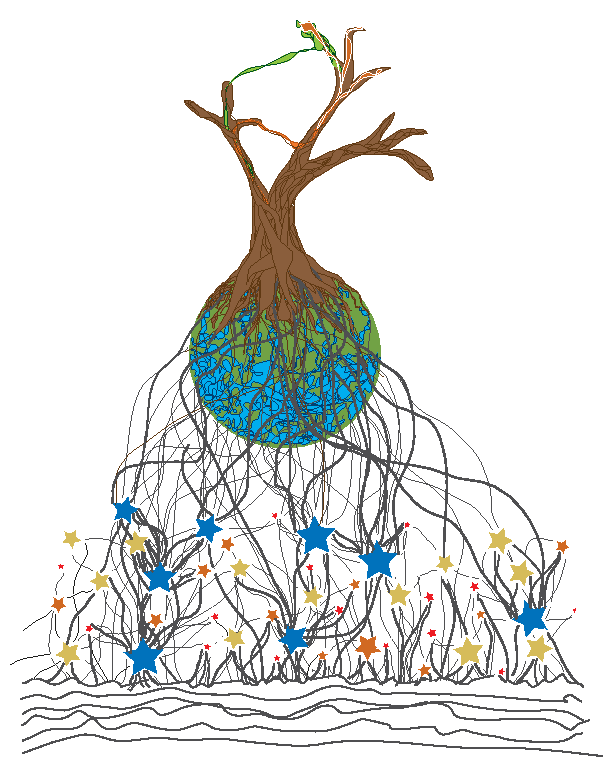
\includegraphics[width=0.6\textwidth]{gfx/front_cover} \\ \bigskip  
% \vspace{1cm}

\large \textit{A thesis submitted for the degree of \degreename}\\[0.7cm] % University requirement text
%\textit{in the}\\[0.4cm]
% \groupname\\
\deptname\\ % Research group name and department name
%\univname % University name

%{\small Draft (\today)}\\[2cm] % Date
%\includegraphics{Logo} % University/department logo - uncomment to place it


\includegraphics[width=5cm]{gfx/ANU_LOGO_cmyk_56mm}

{\normalsize September, 2022}\\[2cm] % Date
\vspace*{\fill}

\copyright Copyright by \authorname  2022

All Rights Reserved
\end{center}

\end{titlepage}

%----------------------------------------------------------------------------------------
%	DECLARATION PAGE
%----------------------------------------------------------------------------------------

\begin{declaration}
%\addchaptertocentry{\authorshipname} % Add the declaration to the table of contents
\begingroup
\large
\noindent This thesis is an account of research undertaken between January 2018 and September 2022 at the College of Engineering and Computer Sciences, The Australian National University, Canberra, Australia. 

%Except where acknowledged in the customary manner, all material presented in this dissertation including figures and photographs are original and have not been submitted in whole or part for a degree in any university.

The work presented in this thesis is that of the candidate alone, except where indicated by due literature reference and acknowledgements in the text. It has not been submitted in whole or in part for any other degree at this or any other university.

The development of ideas and research was undertaken with guidance from my primary supervisors Robert Williamson and Cheng Soon Ong, and the thesis was written by myself. The overall direction of the research was developed in collaboration with my supervisors, who also provided a lot of detailed feedback on my work along the way. The original results presented here were primarily my work.

\bigskip
\vspace{1cm}
\begin{flushright}
\authorname\\
\today
\end{flushright}
\endgroup
\end{declaration}
\vspace{3cm}
% \begingroup
% \footnotesize\emph{{Cover: Figure 1 from \fullcite{Lineweaver2012AnnRev}}}
% \endgroup
\cleardoublepage

% \begin{declaration}
% \addchaptertocentry{\authorshipname} % Add the declaration to the table of contents
% \noindent I, \authorname, declare that this thesis titled, \enquote{\ttitle} and the work presented in it are my own. I confirm that:

% \begin{itemize} 
% \item This work was done wholly or mainly while in candidature for a research degree at this University.
% \item Where any part of this thesis has previously been submitted for a degree or any other qualification at this University or any other institution, this has been clearly stated.
% \item Where I have consulted the published work of others, this is always clearly attributed.
% \item Where I have quoted from the work of others, the source is always given. With the exception of such quotations, this thesis is entirely my own work.
% \item I have acknowledged all main sources of help.
% \item Where the thesis is based on work done by myself jointly with others, I have made clear exactly what was done by others and what I have contributed myself.\\
% \end{itemize}
 
% \noindent Signed:\\
% \rule[0.5em]{25em}{0.5pt} % This prints a line for the signature
 
% \noindent Date:\\
% \rule[0.5em]{25em}{0.5pt} % This prints a line to write the date
% \end{declaration}

% \cleardoublepage

%----------------------------------------------------------------------------------------
%	QUOTATION PAGE
%----------------------------------------------------------------------------------------

% \vspace*{0.2\textheight}

% \noindent\enquote{\itshape Thanks to my solid academic training, today I can write hundreds of words on virtually any topic without possessing a shred of information, which is how I got a good job in journalism.}

% \hfill Dave Barry

%----------------------------------------------------------------------------------------
%	ACKNOWLEDGEMENTS
%----------------------------------------------------------------------------------------

\begin{acknowledgements}
\addchaptertocentry{\acknowledgementname} % Add the acknowledgements to the table of contents
\vspace{0.4cm}
\begingroup
\normalsize
The research in this thesis would not have been possible without my primary supervisors Robert Williamson, Cheng Soon Ong and Amanda Barnard. They have all been extremely patient, they have provided enormous amounts of good advice and discussion about technical details of my research, writing and about where I might be trying to go in the end and how I might get there. This research was motivated by a seemingly compelling idea about the relationship between causal models and the purpose of causal modelling, and a great deal of time was taken up with struggling to fashion this idea into a coherent and comprehensible theory. I sometimes doubted whether there was a worthwhile payoff in the end, or whether I would be able to find it. The support from my supervisors in all its forms helped me to find a path forward and to believe it was still a path worth following.

I would also like to thank Parastoo Sadeghi, Tom Everitt, Sarita Rosenstock and Zhen-Yue Chin for listening to my ideas, offering feedback, encouragement and organisational advice, and Amardeep Wander for offering flexible employment throughout much of the time I have been working on this research. Both the flexibility and the employment are deeply appreciated. I would also like to thank my parents Julie Permezel and Dennis Johnston for their help with childcare at the end of writing.

I would finally like to express my deepest gratitude to my partner, Mevlana Adil, who has gone far out of her way to support me both to commence and to finish writing this thesis through a few wild years. Without her love and support finishing would have been much less likely. I also want to acknowledge my daugher Ana\"is for her understanding and cooperation beyond my expectations for a person her age.
\endgroup
\end{acknowledgements}

%----------------------------------------------------------------------------------------
%	ABSTRACT PAGE
%----------------------------------------------------------------------------------------

\begin{abstract}
\addchaptertocentry{\abstractname} % Add the abstract to the table of contents
\begingroup
\normalsize
Mathematical formalisms of causal inference usually depend on theories of causation, and are often used to analyse problems of data-driven decision making. We show that it is possible to formalise data-driven decision problems and analyse key assumptions using a more minimal theory that aims only to satisfy the requirements of decision makers, and not to additionally offer an account of causation.

Motivated by the literature on decision theory, we consider maps from a decision maker's set of options to probability distributions on a common sample space to be the object of our study, which we call a \emph{decision model}. We extend standard probability theory to a theory of \emph{probability sets} to support reasoning with models of this type. We also make use of a string diagram notation for stochastic functions.

Drawing nontrivial conclusions from decision making models requires nontrivial assumptions. Such assumptions are usually formulated using a theory of causation. We propose that symmetries of decision models may cut out this ``causal detour''. In particular, we investigate the assumption that a sequence of pairs is related by \emph{conditionally independent and identical responses} (henceforth: CIIR sequences). We show that this assumption is equivalent to the assumption that different infinite sequences of pairs are, in a certain sense, interchangeable -- an assumption that we argue is usually unreasonable if the pairs in question are observable.

We show how causal models formulated using both the causal Bayesian network and potential outcomes approach can be represented as decision models with CIIR sequences involving latent variables. The two approaches each require a different extra assumption in order to be made compatible with ours. Causal Bayesian networks require a specification of how to ``unroll'' a structural model into a sequential model. A potential outcomes model requires a specification of how the decision maker's options relate to the rest of the model. Both approaches avoid the criticism of CIIR sequences we raise as the pairs in question are not fully observable.

The assumption of \emph{precedent} is the assumption that ``whatever we can do has been done before'', and is weaker than the assumption of CIIR sequences. We show that the assumption of precedent in conjunction with a technical condition of \emph{regular relationships between conditionals} can yield a conclusion of CIIR sequences when the data displays the right kind of conditional independence. The aforementioned technical condition is similar to a number of assumptions found in the literature that license the conclusion of a directed causal relationship from certain features of the given data. We speculate the assumption of precedent may offer an alternative way to understand directed causal relationships.
\bigskip

% \textbf{Keywords:} \keywordnames

\endgroup
\end{abstract}

%----------------------------------------------------------------------------------------
%	LIST OF CONTENTS/FIGURES/TABLES PAGES
%----------------------------------------------------------------------------------------

% \renewcommand{\listfigurename}{Figures}
% \renewcommand{\listtablename}{Tables}

\begin{spacing}{0.94} 
\tableofcontents % Prints the main table of contents
\end{spacing}

% \listoffigures % Prints the list of figures
% \listoftables % Prints the list of tables
% \listoflistings % Prints the list of python codes

%----------------------------------------------------------------------------------------
%	ABBREVIATIONS
%----------------------------------------------------------------------------------------

% \begin{abbreviations}{ll} % Include a list of abbreviations (a table of two columns)
% \textbf{ANU}&\textbf{A}ustralian \textbf{N}ational \textbf{U}niversity\\

% \end{abbreviations}

%----------------------------------------------------------------------------------------
%	PHYSICAL CONSTANTS/OTHER DEFINITIONS
%----------------------------------------------------------------------------------------

% \begin{constants}{lr@{${}={}$}l} % The list of physical constants is a three column table

% % The \SI{}{} command is provided by the siunitx package, see its documentation for instructions on how to use it

% Speed of Light & $c_{0}$ & \SI{2.99792458e8}{\meter\per\second} (exact)\\
% %Constant Name & $Symbol$ & $Constant Value$ with units\\

% \end{constants}

%----------------------------------------------------------------------------------------
%	SYMBOLS
%----------------------------------------------------------------------------------------

\begin{symbols}{ |p{0.25\linewidth}|p{0.19\linewidth}|p{0.25\linewidth}|p{0.19\linewidth}|}  % Include a list of Symbols (a three column table)
\hline
  Name & Notation & Meaning & Reference \\
 \hline
 \endhead
 \hline
 \endfoot
 \endlastfoot
  \multicolumn{4}{|l|}{\textbf{Miscellaneous symbols}}\\
 \hline
 Numbers from $m$ to $n$ & $[m,n]$ & The set of natural numbers $\{m,m+1,...,n\}$ &\\
 Numbers up to $n$ & $[n]$ & The set of natural numbers $\{1,2,...,n\}$ & \\
 Complement of $[n]$ & $[n]^{\complement}$ The set $\mathbb{N}\setminus[n]$  & \\
 Iverson bracket & $\llbracket \cdot \rrbracket$ & Function equal to 1 if $\cdot$ is true, false otherwise & \\
 Directed graphs & $\graph{G},\node{V},\node{E}$ & Directed graph $\graph{G}$, set of nodes $\node{V}$, set of edges $\node{E}$ & Definition \ref{def:dir_graph} \\
 \hline
 \addlinespace
 \multicolumn{4}{|l|}{\textbf{Probability theory}}\\
 \hline
 Variable & $\RV{X}$ & Measurable function $(\Omega,\sigalg{F})\to(X,\sigalg{X})$ & Definition \ref{def:variable} \\
 Trivial variable & $*$ & Any single-valued random variable & Definition \ref{no:single_valued} \\
 Variable sequence & $(\RV{X},\RV{Y})$ & The variable given by $\omega\mapsto (\RV{X}(\omega),\RV{Y}(\omega))$ & Definition \ref{def:seqvar}\\
 Probability measure & $\prob{P}\in \Delta(\Omega)$ & Countably additive measure on $(\Omega,\sigalg{F})$ with $\prob{P}(\Omega)=1$ & Definition \ref{def:prob_meas}\\
 Set of probability measures & $\Delta(\Omega)$ & Set of probability measures on $(\Omega,\sigalg{F})$ & Notation \ref{no:prob_meas_set}\\
 Markov kernel & $\kernel{K}:X\kto Y$ & Measurable map from $(X,\sigalg{X})$ to probability measures on $(Y,\sigalg{Y})$ & Definition \ref{def:markov_kern}\\
 Dirac measure & $\delta_x$ & Probability measure where $\delta_x(A)=1$ if $x\in A$, $0$ otherwise & Definition \ref{def:dirac_meas}\\
 Markov kernel associated with a function & $\kernel{F}_{f}$ & Markov kernel associated with $f:X\to Y$ that maps $x\mapsto \delta_{f(x)}$ & Definition \ref{def:mkern_func}\\
 Marginal distribution & $\prob{P}^{\RV{X}}$ & $\prob{P}\kernel{F}_{\RV{X}}$ & Definition \ref{def:pushforward}\\
 Conditional distribution & $\prob{P}^{\RV{Y}|\RV{X}}$ & Arbitrary Markov kernel $X\kto Y$ such that $\prob{P}^{\RV{XY}}(A\times B) = \int_A \prob{P}^{\RV{Y}|\RV{X}}(B|x)\prob{P}^{\RV{X}}(\mathrm{d}x)$ & Definition \ref{def:disint} \\
 Conditional independence & $\RV{X}\CI_{\prob{P}}\RV{Y}|\RV{Z}$ & $\prob{P}^{\RV{X}|\RV{YZ}}(A|y,z)$ does not depend on $z$ & Definition \ref{def:ci}\\
 Uniform conditional probability & $\prob{P}_A^{\RV{Y}|\RV{X}}$ & Arbitrary Markov kernel $X\kto Y$ that is a conditional distribution for every $\alpha\in A$ & Definition \ref{def:cprob_pset}\\
 Kernel product & $\kernel{K}\kernel{L}$ & The Markov kernel given by $(A|x)\mapsto \int_Y \kernel{L}(A|y)\kernel{K}(\mathrm{d}y|x)$ & Definition \ref{def:kproduct}\\
 Semidirect product & $\kernel{K}\odot \kernel{L}$ & The Markov kernel given by $(A\times B|x)\mapsto \int_A \kernel{L}(B)|y)\kernel{K}(\mathrm{d}y|x)$ & Definition \ref{def:copyproduct}\\
 Permuted sequence & $\RV{Y}_\rho$ & Given $\RV{Y}:=(\RV{Y}_i)_{i\in\mathbb{N}}$, $\RV{Y}_\rho:=(\RV{Y}_{\rho(i)})_{i\in\mathbb{N}}$ & \\
\hline
\addlinespace
\multicolumn{4}{|l|}{\textbf{String diagrams}}\\
\hline
 Identity map & $\mathrm{Id}_X$ & Markov kernel associated with the identity function $X\to X$ & Definition \ref{def:ident_k}\\
 Erase map & $\mathrm{Del}_X$, $\stopper{0.5}$ & Markov kernel associated with the trivial variable $*_X:X\to \{*\}$ & Definition \ref{def:erase}\\
 Swap map & $\mathrm{Swap}_{XY}$, $\swap{0.5}$ & Markov kernel associated with the function that swaps its inputs $(x,y)\mapsto (y,x)$ & Definition \ref{def:swap}\\
 Swap according to permuation & $\mathrm{Swap}_\rho$ & Markov kernel that swaps inputs in a manner specified by permuation $\rho$ &\\
 Copy map & $\mathrm{Copy}_{X}$, $\splitter{0.2}$ & Markov kernel associated with the function that makes two copies of its inputs & Definition \ref{def:copy}\\
\hline
\addlinespace
\multicolumn{4}{|l|}{\textbf{Probability sets and decision models}}\\
\hline
Decision model & $(\prob{P}_\cdot,(\Omega,\sigalg{F}),C)$ & An option set $C$, a sample space $(\Omega,\sigalg{F})$ and a stochastic map from options to the sample space & Definition \ref{def:dec_model}\\
Probability set & $\prob{P}_A$ & A collection of probability measures $\{\prob{P}_\alpha|\alpha\in A\}$ on a common sample space & Definition \ref{def:prob_set}\\
Option set & $C$ & Interpreted as the set of options available to a decision maker & Definition \ref{def:dec_model}\\
Nonstochastic variable & $\phi$ & Function defined on the option set $C\to A$ & Definition \ref{def:nonstoc_var}\\
Complementary variables & $(\phi,\xi)$ & Sequence of nonstochastic variables that induces an invertible function & Definition \ref{def:comp_var}\\
Extended conditional independence & $\RV{X}\CI^e_{\prob{P}_C}(\RV{Y},\phi)|(\RV{Z},\xi)$ & Generalisation of conditional independence to decision models & Definition \ref{def:eci_orig}\\
Choice variable & $\text{id}_C$ & Identity function on option set $C$; corresponds to the choice made by decision maker & \\
Tabular conditional & $\RV{Y}^X$ & Variable with the property that $\RV{Y}=\sum_{x\in X} \llbracket \RV{X}=x\rrbracket \RV{Y}^x$; not necessarily interpretable as potential outcomes & Definition \ref{def:tab_cd}\\
Input-output model & $(\prob{P}_C,\RV{D},\RV{Y})$ & Shorthand for $((\prob{P}_\cdot,(\Omega,\sigalg{F}),(C,\sigalg{C})),\RV{D},\RV{Y})$ with sequence of inputs $\RV{D}$ and corresponding outputs $\RV{Y}$ & Definition \ref{def:seq_io}\\
\hline
\end{symbols}

%----------------------------------------------------------------------------------------
%	DEDICATION
%----------------------------------------------------------------------------------------

% \dedicatory{For/Dedicated to/To my\ldots} 




%----------------------------------------------------------------------------------------
%	THESIS CONTENT - CHAPTERS
%----------------------------------------------------------------------------------------

\mainmatter % Begin numeric (1,2,3...) page numbering

\pagestyle{thesis} % Return the page headers back to the "thesis" style

% Include the chapters of the thesis as separate files from the Chapters folder
% Uncomment the lines as you write the chapters

\chapter{Habitable Worlds}\label{ch:HabitableWorlds}
This chapter was published as
\begin{description}
	\item \fullcite{Lineweaver2012AnnRev}
	%\item Section~\ref{sec:HabEnergies} has been extended.
\end{description}
\section*{Abstract}
We review the habitability of our Earth and other Earth-like planets. Understanding habitability and using that knowledge to locate the nearest habitable planet may be crucial for our survival as a species. To evaluate remotely the habitability of the increasing number of Earth-like exoplanets, we need to understand which features of our own planet enabled the origin and evolution of life – and if these features are universal. We discuss the habitability of Earth, the habitability of planets orbiting other stars, and the habitability of our galaxy. We profile the `bioshell' - the $\sim$\,1\% volume of our planet, which is inhabited by life and describe temperature and nutrient deserts where there is little biomass. The inhabited and uninhabited regions on Earth suggest that the presence of liquid water in a narrow temperature range is the main constraint that can be used in a habitability classification scheme for rocky planets.

We review current ideas about the microbiology and bioenergetics of the earliest terrestrial life forms and find that the conditions for life's emergence may be different and more specific than the broader conditions to which life can adapt. Since life and its environment co-evolve, we propose the dynamic concept of an `Abiogenesis Habitable Zone', where life can get started and which, upon continual modification by life, transitions into a 'Habitable Zone'. Our compilation of recent exoplanet detections suggests that the fraction of stars with planets is $\sim$\,100\% and the fraction of stars with a rocky planet in the habitable zone could be comparably large. Recent discoveries suggest that there are at least 10 times as many Earth-sized planets as Neptune sized planets, which in turn are 10 times more abundant than Jupiter-sized planets. Although the process of rocky planet formation and supply of water to terrestrial planets, seems to be a common product of star formation, the water content of a rocky planet is probably highly variable. This variability can be used to classify their habitability, e.g., ocean planets, Earth-like planets, and desert planets.

\clearpage

\begin{flushright}
		\textit{The Sun with all those planets revolving around it\\ and dependent on it, can still ripen a bunch of grapes\\ as if it had nothing else in the universe to do. \\
		--- Galileo Galilei}
	\end{flushright}

The universe is filled with stars like our Sun \cite{Robles2008}, rocky planets like our Earth \citep{Howard2012}, water like in our oceans \citep{Mottl2007}, amino acids like those that make up our proteins, and all the other ingredients for life \citep{Pizzarello2007}. But is the universe filled with anything we would recognize as life \citep{Lineweaver2006}\,? \citet{DeDuve1995} has argued that the initial deterministic nature of proto-biochemistry makes life a ``cosmic imperative'' built into the chemistry of the universe, and we should therefore expect life to be common in the universe.

%%%%%%%%%%%%%%%%%%%%%%%%%%%%%%%%%%%%%%%%%%
\begin{figure}[!hbt]
	\centering
	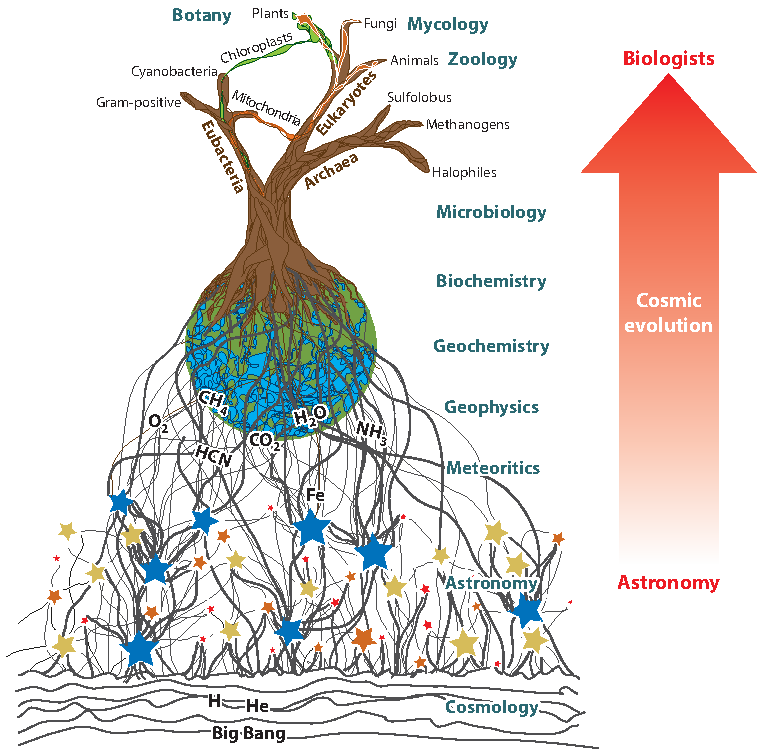
\includegraphics[width=1\linewidth]{figures/AnnRevs/AR1.pdf}
	\caption[Cosmic Evolution]{The emergence of biologists from astronomy. Starting from the big bang at the bottom, deterministic physical sciences set the context for the emergence of life. The resulting biologists (animals) at the top of the tree \citep[\eg][]{Pace1997, Hedges2009} have constructed the brown phylogenetic tree based on the molecular fossils inside the DNA of the inhabitants of the biosphere. The terrestrial tree of life took root approximately four billion years ago. We review the features of rocky planets that are implicated in the ability to give root to, and maintain, a tree of life. 
	}
	\label{fig:AR1}
\end{figure}

%%%%%%%%%%%%%%%%%%%%%%%%%%%%%%%%%%%%%%%%%%
\begin{figure}[!hbt]
	\centering
	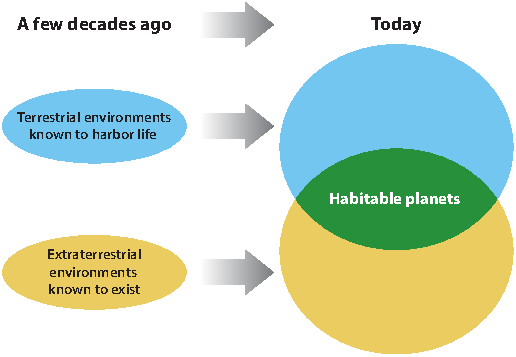
\includegraphics[width=1\linewidth]{figures/AnnRevs/AR2.pdf}
	\caption[Emergence of habitable planets.]{Emergence of habitable planets. Habitable planets are emerging from the increasing overlap of two sets of environments: the increasingly large set of terrestrial environments known to harbor life and the increasingly large set of extraterrestrial environments on the newly detected rocky exoplanets. The overlap of these research fields bolsters expectations that the universe may be filled with habitable planets.}
	\label{fig:AR2}
\end{figure}

Terrestrial life emerged from nonlife approximately four billion years ago \citep{Battistuzzi2004,Sleep2008} (Figure~\ref{fig:AR1}). Descriptions of where this happened include warm little ponds \citep{Darwin1871}, hot hydrothermal vents \citep{Wachtershauser2006, Martin2008}, and cold little ponds \citep{Bada1994}. Scenarios for how life emerged include a prebiotic soup under a reducing atmosphere \citep{Oparin1924, Miller1953} and some form of semi-deterministic molecular chemistry \citep{Dyson1999, Segre2000} that evolved into auto-catalytic reactions \citep{Eigen1971} and produced replicating molecules \citep{Cairns-Smith1982, Gesteland1999}, proto-metabolisms \citep{Pascal2006}, and cell membranes \citep{Deamer2010}. Despite the variety of these scenarios, some common threads represent our best estimates of what we might expect to share with extraterrestrial life. We can expect extraterrestrial life to be based on Darwinian evolution and the most fundamental features of terrestrial biochemistry \citep{Feinberg1978, Pace2001, Morris2003, Benner2004, DeDuve2007, Lineweaver2012}. Noncoincidentally, these are the same features that are often used to define life \citep[\eg][]{Schrodinger1944, Sagan1970, Joyce1994, Leach2006}.
 
During the past few decades, the exploration of some extreme environments on Earth has uncovered extremophile microbial life in conditions previously thought to be too hostile for life. These discoveries have expanded the variety of terrestrial environments known to harbor life \citep{Rothschild2001, Stetter2006, Shock2007, Baross2007, Madigan2010, Pedersen2010}. During the same few decades, progress in the characterization of the planets and moons of our Solar System, and progress in the detection of a wide variety of exoplanets in orbit around an increasingly large fraction of stars, has broadened the range of known extraterrestrial environments (Sections \ref{sec:FractionPlanets} and \ref{sec:HabitableTemperatures}). The growing overlap of these two sets of environments suggests that habitable planets are abundant (Figure~\ref{fig:AR2}). This increases the probability of finding some kind of extraterrestrial life.

The number of papers and conferences reporting new exoplanet and extremophile discoveries, and those grappling with the issue of planetary habitability, has enormously increased. Recent reviews of habitability include \citet{Kasting2003}, \citet{Gaidos2005}, \citet{Hoehler2007a}, \citet{Fishbaugh2007}, \citet{Kopparapu2013} and \citet{Kasting2014}.

This review provides an overview of habitability and focuses on what we know about the habitability of Earth, the habitability of planets orbiting other stars, and the habitability of our galaxy. It synthesizes facts and current ideas about the microbiology of the earliest terrestrial life and the latest findings of planet hunters. It is organized as follows: Section \ref{sec:HZones} reviews the limits of terrestrial life and illustrates where life is found, and is not found, on the habitable planet that we know best—Earth. We discuss energy constraints on life and how the conditions for life's emergence may be different and more specific than the broader conditions to which life can adapt. Section \ref{sec:FractionPlanets} presents the increasingly compelling evidence that planets in general, and rocky planets in particular, are a common product of star formation. Section \ref{sec:HabitableTemperatures} discusses the habitability of the most Earth-like exoplanets and the traditional circumstellar habitable zone (HZ). Section \ref{sec:WaterDel} reviews the supply of water to terrestrial planets. Finally, Section \ref{sec:GHZ} reviews work on the galactic HZ and discusses a variety of habitability issues.

\clearpage
\section{The Habitable Zones on Earth}\label{sec:HZones}
Because habitability is about the complex relationship between life and environment, we start close to home with a discussion of the relationship between terrestrial life and terrestrial environments. The close fit between our requirements and what Earth can provide is not coincidental. Earth and the life on it have coevolved. However, life is not infinitely adaptive. Some parts of Earth are habitable and some, even after approximately four billion years of evolution, are not. Life as we know it has limits, and we can explore these limits most easily on Earth.

%%%%%%%%%%%%%%%%%%%%%%%%%%%%%%%%%%%%%%%%%%
\begin{figure}[!hbt]
	\centering
	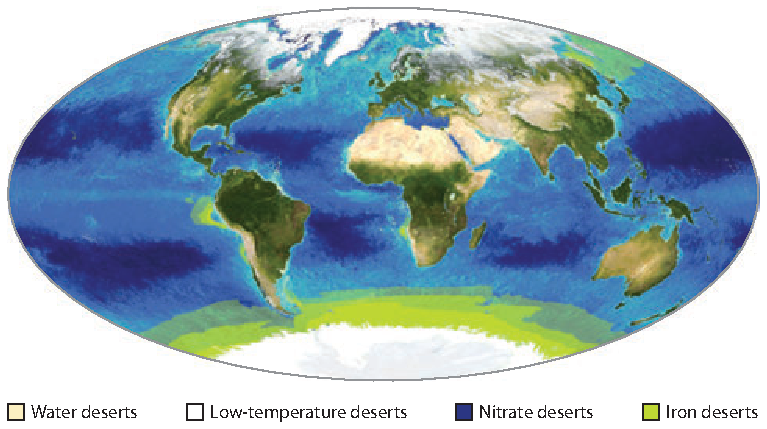
\includegraphics[width=0.9\linewidth]{figures/AnnRevs/AR3.pdf}
	\caption[Deserts on Earth]{Four deserts on Earth's surface. Life is not evenly distributed over the surface of Earth. There are water deserts (sandy brown), low-temperature deserts (white), nitrate deserts (dark blue), and iron deserts (light green), where the abundance of life is significantly lower than in surrounding regions. This map was constructed with data from \citet{Stockli2005,McClain2006}.}
	\label{fig:AR3}
\end{figure}

In a specific region, when some requirement for life is outside the optimal range for life, the total biomass in that region is low (Figure~\ref{fig:AR3} presents these regions). We generically call such regions deserts. Low rainfall makes water deserts. Low temperatures make low-temperature deserts at Earth's poles. Far from land, in mid-oceanic gyres (where windblown dust and aerosols are at a minimum \citep{Duce1991}), low nitrate levels produce nitrate deserts. 

Chlorophyll maps of the ocean \citep{McClain2006,McClain2009} show regions where, despite ample water, photons, and nitrates, there are low concentrations of chlorophyll. Iron fertilization experiments in these enigmatic high-nitrate-low-chlorophyll regions found that the biomass was iron limited, rather than phosphate limited or limited by some other nutrient \citep{Falkowski1998, Smetacek2008}. Such iron deserts have been identified in the Southern Ocean, the northwest Pacific, and the eastern equatorial Pacific. Low-phosphate regions overlap significantly with nitrate deserts \citep{Garcia2006}. Because the elements H, O, C, N, P, and S make up $\sim$\,98\% (by mass) of life \citep{Lineweaver2012}, one might expect analogous C and S deserts.

The subtle variations of biomass over the horizontal surface (Figure~\ref{fig:AR3} ) are dwarfed by the nonsubtle variations of biomass in the vertical direction. The terrestrial biosphere is a thin bioshell whose thickness ($\sim$\,10 km) is $\sim$\,1/600 of Earth's $\sim$\,6,400 km radius. Figure~\ref{fig:AR4}  is a vertical profile of terrestrial biomass. Low temperatures and low densities prevent life from living permanently in air or on the highest mountains (low-temperature deserts). High temperatures prevent life from existing more than $\sim$\,5 kilometers underground, because the average continental geothermal gradient of 20{-}30\textcelsius per km reaches the upper temperature limit of life (122\textcelsius{}, \citep{Takai2008}) at approximately that depth. (Shield gradients and those above subduction zones can be as low as $\sim$\,$10$\textcelsius{} per km.) Thus, the interior of Earth is a spherical high-temperature desert. The bioshell is thin because life is kept squeezed into a narrow HZ between a high-temperature desert below and a low-temperature desert above (Figures \ref{fig:AR4} and \ref{fig:AR5}). 

%%%%%%%%%%%%%%%%%%%%%%%%%%%%%%%%%%%%%%%%%%
\begin{figure}[!hbt]
	\centering
	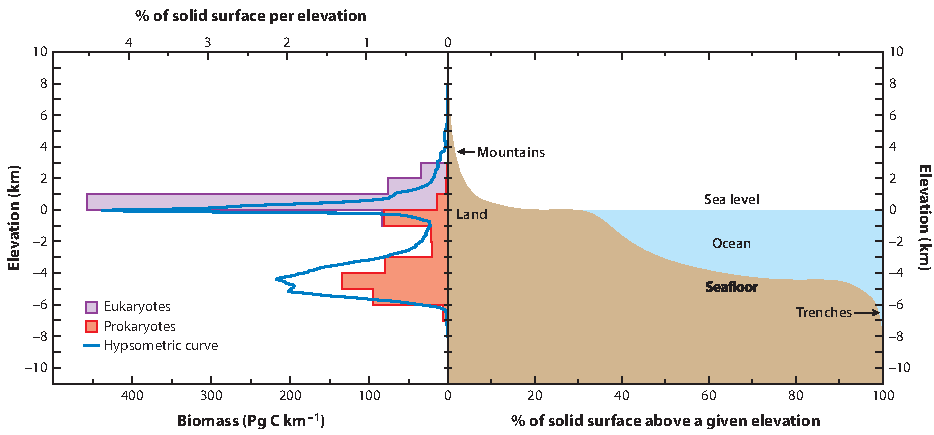
\includegraphics[width=0.9\linewidth]{figures/AnnRevs/AR4.pdf}
	\caption[Terrestrial bioshell]{Vertical profile of biomass in the thin terrestrial bioshell ($\pm$10 km). The hypsographic curve on the right shows the fraction of Earth's solid surface above a given elevation. For example, 30\% of the solid surface is above sea level, whereas the remaining 70\% is below sea level. The hypsometric curve on the left (blue line) \citet{Perotti2011} shows the fraction of Earth's solid surface at any given elevation. The histogram on the left shows our estimate of the vertical profile of terrestrial biomass (total carbon in terrestrial life forms) derived from combining data from \citet{Whitman1998,Houghton2003}. Since the publication of the paper presented in this chpater, \citet{Kallmeyer2012} analysed a more diverse range of sediment samples and estimate that the biomass in sub-seafloor sediments is 10-45\% lower than estimates used by \citet{Whitman1998}. \citet{Jorgensen2012,Hinrichs2012} and further analysis by \citet{Mcmahon2014} confirm the overestimation by \citet{Whitman1998}. However, we find that even with the new estimates our main conclusions of the relative distribution of prokaryotic and eukaryotic life is not challenged.}
	\label{fig:AR4}
\end{figure}

%%%%%%%%%%%%%%%%%%%%%%%%%%%%%%%%%%%%%%%%%
\begin{figure}[!hbt]
	\centering
	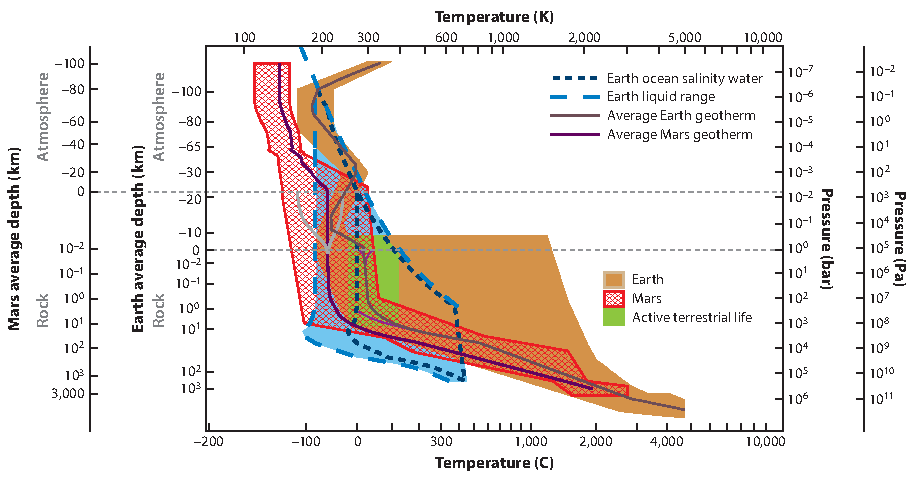
\includegraphics[width=0.9\linewidth]{figures/AnnRevs/AR5.pdf}
	\caption[Uninhabited water on Earth \& Mars]{Uninhabited water on Earth and the potential biosphere of Mars. This pressure-temperature phase diagram is a superposition of the region where H$_{2}$O is liquid (blue), all terrestrial environments (brown), inhabited terrestrial environments (green), and all Martian environments (hatched red). Notice the large regions of uninhabited terrestrial liquid water that is either too cold ({-}80\textcelsius{} < T < {-}20\textcelsius{}) or too hot (122\textcelsius{} < T < 400\textcelsius{}) for life. The $\pm$10 km vertical extent of the green area corresponds to the elevation range of the biomass profile in Figure~\ref{fig:AR4}. The shape of the green area shows that the presence of liquid water and the {-}20\textcelsius{} to {+}122\textcelsius{} temperature range are the dominant variables determining habitability. These inhabited and uninhabited terrestrial environments, set by the need for liquid water and a specific range of temperature, are our best guides to exoplanet habitability. Figure from \citet{Jones2011}. See also \citet{Mottl2007,Jones2010,Jones2012,Cockell2011}.}
	\label{fig:AR5}
\end{figure}

Terrestrial biomass is approximately evenly divided between eukaryotes (55\%; Figure~\ref{fig:AR4}, light purple) and prokaryotes (45\%; Figure~\ref{fig:AR4}, orange). Biomass is also roughly evenly divided between above sea level (56\%) and below sea level (44\%). Of Earth's eukaryotic biomass, 99.5\% is on land \citep{Sundquist2014}. About 96\% of prokaryotic biomass is below sea level, mostly in seafloor sediments \citep{Whitman1998}. The oxygenic photosynthesis that powers most of the eukaryotic life on land was a relatively late adaptation \citep{Kiang2007, Sleep2007}, as was the ability to colonize the land \citep{Battistuzzi2004}. Five hundred million years ago, there was land but little eukaryotic life on it. Thus, for approximately the first three billion years, the profile of terrestrial biomass may have resembled the current prokaryotic profile (Figure~\ref{fig:AR4}, orange).

\subsection{The Abiogenesis Habitable Zone}
As we learn more about the origin of life, we can start to define an abiogenesis habitable zone (AHZ) where the requirements for life's emergence are met. The habitability requirements for the origin of life may be substantially different from, and more specific than, the requirements to maintain life on a planet—think of the difference between a spark plug to start an engine and a carburetor to supply it with fuel. If you shine light onto a vat of HOCNPS, or bubble molecular hydrogen through a flask of amino acids, life does not spontaneously emerge. For a planet to manage the transition from the nonliving to the living\,-\,to qualify as an AHZ\,-\,juxtapositions and flows of specific combinations of molecules are needed to produce auto-catalytic reactions and proto-metabolisms that can tap into either the flow of redox pairs or photons \citep{DeDuve1995, Lane2010}.

Once life begins, organisms do not just passively adapt to preexisting environments. They actively change and construct the world they live in \citep{Odling-Smee2003}. The evolutionary history of life on Earth can be written in terms of how organisms have modified their environments. From the oxygenation of the atmosphere to the creation of beaver dams, life modifies its environment. But life also modifies itself and adapts to fit the environment—evolving, for example, spores to survive dry conditions, antifreeze for survival at low temperatures, and salt pumps to survive at high salinity. Whether life adapts to fit an environment or modifies an environment to be able to survive, the result is the same: The initial specific AHZ is widened (Figure~\ref{fig:AR6}). Through its management of the greenhouse and its partitioning of reductants and oxidants, the activity of life increases the range of inhabited environments \citep{Nisbet2007,Hazen2008}. 

%%%%%%%%%%%%%%%%%%%%%%%%%%%%%%%%%%%%%%%%%%
\begin{figure}[!hbt]
	\centering
	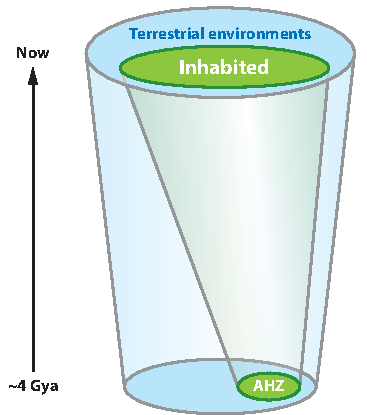
\includegraphics[width=0.5\linewidth]{figures/AnnRevs/AR6.pdf}
	\caption[Abiogenesis habitable zone]{Abiogenesis habitable zone (AHZ). The conditions needed for the origin of life (before life could adapt) are narrower than the broader conditions to which life can adapt.}
	\label{fig:AR6}
\end{figure}

Environments change life-forms, and life-forms change environments. This feedback between life and environment may be so strong that, for a planet to be habitable, it might have to be inhabited. Thus, planetary habitability becomes a dynamic concept with different stages. Habitability begins as a relatively narrow AHZ, completely dependent on the chemistry and other physical characteristics of the planet. Once life emerges and passes the ``Darwinian threshold'' \citep{Woese2002} habitability shifts to a dependence on both the characteristics of the planet and the adaptability of its life-forms. Finally, habitability becomes predominantly dependent on the ability of the inhabitants to regulate their environment. The thermoregulation of Earth over the past four billion years, despite a 30\% increase in solar luminosity, is a possible example of such Gaian regulation \citep{Lovelock1965,Lovelock2000,Lovelock1974,Schneider1991,Schneider2004}. It may be that natural negative-feedback processes, such as the carbon-silicate cycle \citep{Walker1981}, without Gaian regulation, are not conducive to life any more than a nonevolving body would be \citep{Schwartzman1989}. Thus, eventually, habitability becomes a property of life, as much as, or perhaps more than, it is a property of a planet.

The persistence of life on Earth requires liquid water, an appropriate temperature range, nutrients, and an energy source. Self-assembly is an example of an additional requirement for abiogenesis that would be relaxed once life got started (making the AHZ narrower than the HZ). For example, origin-of-life chemists are trying to understand how RNA could self-assemble in the presence of water \citep[\eg][]{Szostak2001}. To self-assemble, dehydration reactions are needed. Cyclic evaporative dehydration could happen near continental hot springs or in warm tidal pools as the kilometer-high tides came in and out every few hours \citep[\eg][]{Lathe2004}. On ocean planets (Section \ref{sec:HabitableTemperatures}), there could be no dehydration reactions because there would be no evaporation from solid surfaces. Thus RNA would not self-assemble and life might not be able to get started on ocean planets. If the self-assembly of RNA required cyclic evaporation, and this assembly was critical to the emergence of life, ocean planets would be lifeless. They would be habitable but uninhabited planets.

\subsection{Habitable Energies}
\label{sec:HabEnergies}
On Earth today, $\sim$\,60\% of the biomass is phototrophic and $\sim$\,40\% is chemotrophic (Figure~\ref{fig:AR4}). Thus, the dominant energy source for life is the solar photon flux. However, when life emerged approximately four billion years ago there may have been much less dry land \citep{Taylor2009} and no eukaryotes. The terrestrial biomass distribution thus may have more closely resembled the current prokaryotic distribution in which the majority of the biomass is not necessarily in the photic zone but at hydrothermal vents at various depths, which were more common approximately four billion years ago \citep{Southam2007,Sleep2010}. Studying the earliest and most fundamental metabolisms of terrestrial life is our best hope for understanding how likely such energy-transducing metabolisms (and thus life) are to emerge elsewhere. Candidates for the earliest metabolisms include two broad categories of primary producers: anoxygenic phototrophs and chemolithotrophs. Chemolithotrophs live off inorganic redox pairs supplied by chemical disequilibria at hydrothermal vents \citep{Nisbet2001,Kelly2006}.

%%%%%%%%%%%%%%%%%%%%%%%%%%%%%%%%%%%%%%%%%%
\begin{figure}[!hbt]
	\centering
	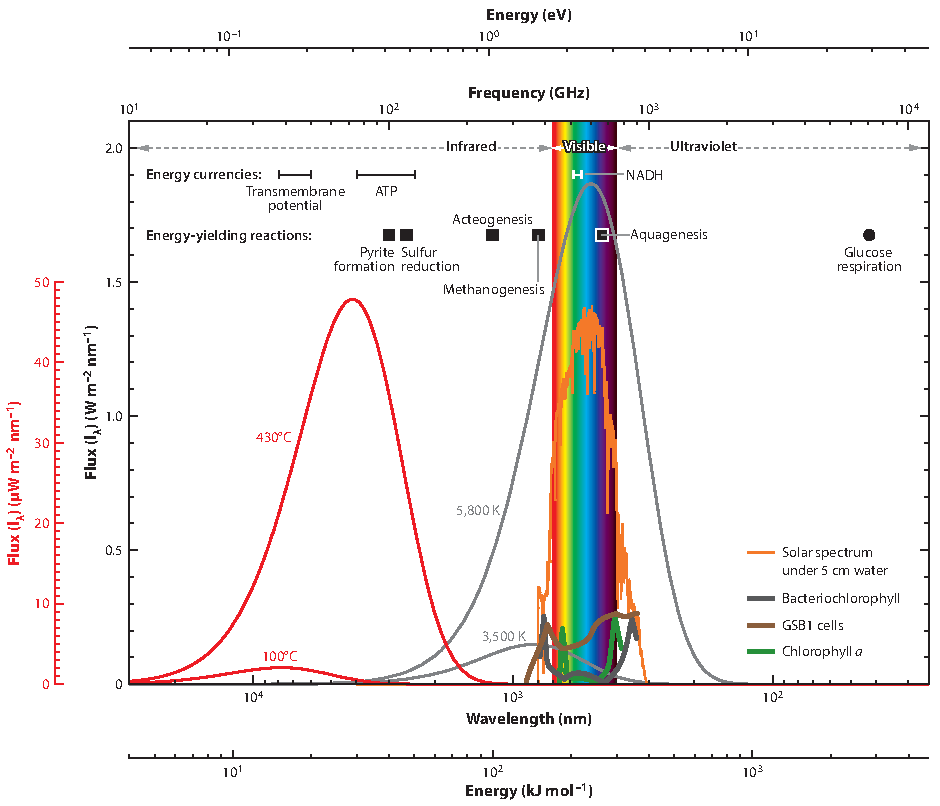
\includegraphics[width=0.9\linewidth]{figures/AnnRevs/AR7.pdf}
	\caption[Energy sources and currencies of life]{Comparison of the photon and redox energy sources of early life with the dominant energy currencies of life. The two sources of energy available to early life were solar photons (represented by the solar spectrum as seen from beneath 5 cm of water (orange)) and inorganic redox pairs available at hydrothermal vents (black squares). The energy obtained from both these sources was converted into the currencies life uses to store or circulate energy (transmembrane potential, ATP, and NADH). Uncertainties indicate the common range of energies associated with these currencies under physiological conditions. Five redox reactions are shown that are candidates for the sources of energy for the first chemolithotrophs (see Table \ref{tab:energycurreny} and \citet{Blank2009}). Blackbody curves are shown for Sun-like G stars and for the most common star in the universe, low-mass M stars such as Gl581 (Section \ref{sec:HabitableTemperatures}). On the left, using a different y-axis, the blackbody spectra of a 430\textcelsius{} hydrothermal vent (or hot spring) fluid and a 100\textcelsius{} fluid represent the native environment of hyperthermophiles. Absorption spectra are shown for two candidates for the earliest anoxygenic photosynthesis: bacteriochlorophyll \citep{Frigaard1996,Madigan2006} and the spectra of intact cells of an obligately photosynthetic bacterial anaerobe (green sulfur bacterium, GSB1) isolated from a deep-sea hydrothermal vent environment \citep{Beatty2005}. The absorption spectrum of eukaryotic chlorophyll a \citep{Cinque2000} and the maximum energy available from oxic glucose respiration are shown for comparison.}
	\label{fig:AR7}
\end{figure}

\begin{table}[!hbt]
	\centering
		\caption[Redox energy currencies and reactions]{Free energies ($\bigtriangleup$G) of redox chemistry of some of the earliest terrestrial energy yielding reactions plotted in Figure~\ref{fig:AR7} \citep{Amend2001,Martin2008,Chang2005,Nicholls1992}. Oxic respiration of glucose is included for comparison.}
	\resizebox{\textwidth}{!}{%
		\begin{tabular}{@{}llcccc@{}}
			\toprule
			{Energy currency} & & {$\bigtriangleup$G (kJ/mol)}  & {Example} \\ \midrule
			Trans-membrane potential                &               & 12-20   & all organisms                                                      \\
			ATP                             &                       & 30-50   & all organisms                                                      \\
			NADH                           &                        & 210-220 & all organisms                                                      \\ \bottomrule
			\\ \toprule
					{Energy yielding reaction} & & {$\bigtriangleup$G (kJ/mol)}  & {Example} \\ \midrule
			FeS(s) + H$_{2}$S(g) $\rightarrow$ FeS$_{2}$(s)+ H$_{2}$(g) &pyrite formation      & 40        & Iron-sulphur world \citep{Wachtershauser1998}                                                \\
			S(s) + H$_{2}$(aq) $\rightarrow$ H$_{2}$S(aq) &sulphur reduction              & 45        & \textit{Sulfurospirillum}, \textit{Pyrodictium occultum}, \textit{Thermococuss} spp.          \\
			4H$_{2}$(aq) + 2CO$_{2}$(aq) $\rightarrow$ CH$_{3}$COOH(aq) + 2H$_{2}$O(l) &acetogenesis & 100       & \textit{Acetogenium kivui}, \textit{Acetobacterium} spp., \textit{Clostridium thermoaceticum} \\
			CO$_{2}$(aq) + 4H$_{2}$(aq) $\rightarrow$ CH4(aq) + 2H$_{2}$O(l) &methanogenesis   & 130       & \textit{Methanococcus}, \textit{Methanobacterium}                                    \\
			H$_{2}$(aq) + 0.5CO$_{2}$ (aq) $\rightarrow$ H$_{2}$O(l)&aquagenesis               & 250       & \textit{Aquifex aeolicus}                                                  \\
			C$_{6}$H$_{12}$O$_{6}$ + O$_{2}$ $\rightarrow$ CO$_{2}$ + H$_{2}$O &oxic respiration              & 2870      & Many bacteria, archaea and eukaryotes including \textit{Homo sapiens}    \\ \bottomrule 
		\end{tabular}
	}
	\label{tab:energycurreny}
\end{table}



Hyperthermophiles are the deepest- and shortest-branched organisms on the phylogenetic tree of life \citep[\eg][]{Pace1997, Lineweaver2003}. Hyperthermophiles gain energy by inorganic redox reactions employing compounds such as H$_{2}$, CO$_{2}$, S$^{0}$, Fe$^{2+}$, and Fe$^{3+}$ \citep{Stetter2006}. Redox reactions in hydrothermal vents and hot springs probably played a dominant role in early metabolism. The earliest life forms were probably chemoheterotrophs that evolved in high-temperature, low-pH, and high-salinity environments resembling hydrothermal vents \citep{Martin2008} or hot springs. The transition of life from a redox-only energy source to a redox and photon energy source is suggested by comparing the energies of different metabolic reactions in Figure~\ref{fig:AR7} \citep{Sleep2008}. The earliest redox reactions -- pyrite formation, sulfur reduction, methanogenesis, and acetogenesis \citep{Wachtershauser1998,Martin2007,Blank2009,Ljungdahl1986} -- provide less energy than photosynthesis. However, these early reactions do provide enough energy to charge transmembrane potentials in a chemiosmotic coupling and convert low-energy molecules such as ADP, NAD$^{+}$, and NADP$^{+}$ to higher-energy molecules such as ATP, NADH, and NADPH \citep{Mitchell1961}. These molecules are universal energy currencies and likely to have been adopted by the earliest organisms.
 
Energy sources based on a redox gradient may have been ubiquitous on the early Earth, particularly because hydrothermal activity may have been more widespread than it is today \citep{Sleep2007}. The similar energies of the earliest metabolic pathways and the availability of the reactants in environments such as hydrothermal vents bolster the case that life began by using energy sources based on redox gradients and over time evolved to perform higher-energy reactions such as oxygenic photosynthesis and oxic respiration. \citet{Canfield2006} claim that the most-active, earliest ecosystems were probably driven by the cycling of H$_{2}$ and Fe$^{2+}$ through primary production conducted by anoxygenic phototrophs.

The absorption spectra of bacteriochlorophylls, which are considered to be more ancient than chlorophylls \citep{Hohmann-marriott2011,Blankenship2010}, and the photosynthetic pigments in green sulfur bacterium (GSB1) peak outside the visible region of the spectrum in the near-IR, where photons can penetrate to some degree through murky water. Although the blackbody emission of hot hydrothermal fluids has far fewer photons in the near-IR than in the mid-IR, they are in sufficient numbers and of high enough energy that GSB1 can photosynthesize and live in a dark environment. Photons of even lower energies ($\sim$\,1,000 nm) are used by purple anoxygenic bacteria \citep{Kiang2007}. Note that all redox reactions in Figure~\ref{fig:AR7} are above the peak energy of the 100\textcelsius{} ambient temperature of a hyperthermophile environment. Any redox reaction that is used by life must satisfy the constraint that the activation energies must be higher than what is available as background energy in the environment \citep{Shock2007}. An upper limit for the temperature at which metabolic activity can take place is set by the temperature at which the molecular dissociation of proteins and membranes takes place.

%%%%%%%%%%%%%%%%%%%%%%%%%%%%%%%%%%%%%%%%%%
\begin{figure}[!hbt]
	\centering
	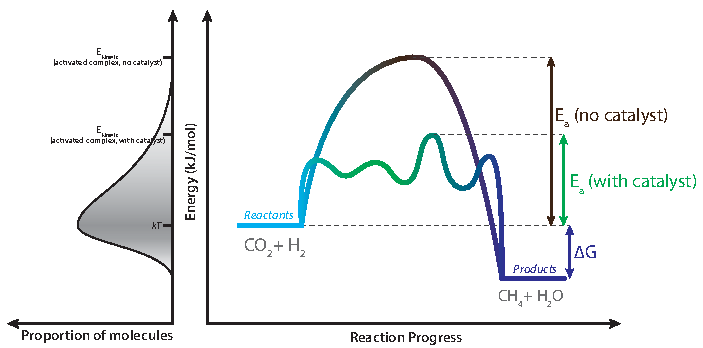
\includegraphics[width=1\linewidth]{figures/Reactions.pdf}
	\caption[Thermodynamics of energy sources for life]{The relationship between environmental kinetic energy kT (represented by the Maxwell-Boltzman distribution on the left), and energies associated with chemical reactions (on the right). Any metabolic reaction used by life must have activation energies higher than kT (the average energy of reactant molecules and the environment) otherwise the reaction would proceed to equilibrium without being mediated by the bio-catalysts of life \citet{Shock2007}. Life makes a living by developing bio-catalysts to lower the activation energy of the reactions of available redox pairs. Metabolism is based on the ability to control the presence of these bio-catalysts \citet{Nealson1999}. Life elsewhere could extract energy from a variety of abiotically produced chemical disequilibria since both the ingredients and the free energy sources (redox or photon based) should be available at the atmosphere:rock-surface or the ocean:rock-surface interfaces on Mars, Titan, Europa and other exoplanetary systems.}
	\label{fig:Reactions}
\end{figure}

If solvents are required for biochemistry, then the temperature at which the solvent remains a liquid, will set the energies of the reactions that biological catalysts can control (Figure~\ref{fig:Reactions}). Typically in terrestrial biochemistry, E$_{a}$(no catalyst) / E$_{a}$(with catalyst) is greater than 10, so the choice of catalyst provides a strong control of the reaction rate \citep{Quinn2014,Alberty2005}. When life was first emerging on Earth and the first catalysts were evolving, this ratio must have been $\sim$\,1, and then gradually evolved to the much larger values (10\,-\,30) that are typical of catalysts used by biota today. 

Energy sources based on redox gradients should be plentiful on rocky planets in circumstellar habitable zones because of the ubiquity of differentially oxidised minerals in the presence of water heated by radiogenic or convective sources in the first approximately 0.5 to 1 billion years of an active wet rocky planet. Over time, life would evolve new catalysts that give access to a wider range of redox pairs and photons, plausibly resulting in a remotely detectable atmospheric biosignature.

If the conditions that permitted terrestrial abiogenesis based on energy-yielding metabolic reactions, such as those plotted in Figure~\ref{fig:AR7}, are not available on other planets, then the search for life elsewhere in the universe may yield the discovery of numerous habitable planets that have remained uninhabited. This is one possible outcome of Mars exploration. The search for life elsewhere in our Solar System has focused on Mars because it is relatively close and because Mars probably contains a lot of subsurface water \citep{Jones2011,Michalski2013}. In Figure~\ref{fig:AR5}, the substantial overlap of the green and red areas represents extensive water at habitable temperatures on Mars. This, combined with much other evidence for water on Mars, suggests that we will find liquid water in the Martian subsurface at temperatures compatible with terrestrial life. If appropriate redox pairs exist, psychrophilic terrestrial life should be able to live between tens of centimeters and ten kilometers beneath the Martian surface \citep{Jones2011}. However, Mars exploration has not yet found any life. In 1976, two Viking spacecraft landed on Mars with life-detection instruments, which returned ambiguous results that have been interpreted as offering no evidence for life \citep{Klein1979,Klein1999,Navarro-Gonzalez2010} \citep[see, however,][]{Levin1981}. Although the Viking mission only attempted to search for active life on the surface (and not in the region below 10 cm where liquid water might be present), there are other potential biosignatures of subsurface life that may be detectable on the surface. One such potential biosignature was recently detected as transitory faint traces of methane \citep{Formisano2004,Krasnopolsky2004,Mumma2009,Lefevre2009}. The debate about whether this methane could be biotic or abiotic seems to be leaning toward an abiotic explanation: Hot olivine exposed to water and CO$_{2}$ undergoes serpentinization and produces methane \citep{Kasting2012,Webster2011}.

NASA's Mars Science Laboratory (MSL), launched on November 26, 2011, has 10 instruments to help determine if life did, or does, exist on Mars. The ongoing exploration of the Martian subsurface is one of the most promising fields where progress in our understanding of habitability can be made. For example, MSL recently detected trace amounts of methane in the Martian atmosphere (in the parts per billion by volume range). The transient spikes in methane abundance suggest episodic production of methane possibly from extant methanogenesis or released from past reservoirs, or both \cite{Webster2015}. Other promising destinations include Jupiter's moons Europa, Ganymede, and Callisto and Saturn's moons Titan and Enceladus. These large moons may have provided wet incubators where life could have emerged (and might still exist). Evidence from the Galileo mission \citep{Spohn2003} suggests that Europa, Ganymede, and Callisto contain a combined volume of liquid water 30–35 times that of Earth's oceans. For reviews of the habitability of our Solar System, see \citet{Shapiro2009} and \citet{McKay2011}. There are also specific papers on the habitability of Europa \citep{Chyba2001,Hand2007}, Enceladus \citep{McKay2008}, Titan \citep{Benner2004,McKay2005,Raulin2008}, and Venus \citep{Grinspoon1997,Svedhem2007}.

\clearpage

\begin{flushright}
	\textit{Since stars appear to be suns, and suns, according to the common opinion, are bodies that serve to enlighten, warm, and sustain a system of planets, we may have an idea of the numberless globes that serve for the habitaton of living creatures.\\
		--- William Herschel}
\end{flushright}

\section{What fraction of stars have terrestial planets}\label{sec:FractionPlanets}

Outside our own Solar System, terrestrial planets or large rocky moons in the circumstellar HZs around other stars are the most likely habitable places. Since 1995, when the first exoplanet was detected around a Sun-like star \citep{Mayor1995}, the fraction of stars with planets has been periodically reported. These are listed in Table \ref{tab:fracstars} and plotted in Figure~\ref{fig:AR8}. The values depend on what fraction of the mass-period parameter space of Figure~\ref{fig:AR9} has been sampled or extrapolated over. Because no technique can sample the entire space, coverage is always incomplete and any reported value such as ``10\% of stars have planets'' is a lower limit—the actual value is larger. Because of this incompleteness, the data are, and always have been, consistent with 100\% of stars having planets. This is represented in Figure~\ref{fig:AR8} by the blue arrows extending from the reported lower limits to 100\%. See \citet{Cassan2012} for supporting evidence from microlensing observations.


\begin{table}[!h]
	\centering
	\resizebox{\textwidth}{!} & \multicolumn{2}{c}{{Mass Range}} & {Orbital limits} & {Detection Technique} \\
 &   & {M$_{min}$} & {M$_{max}$} & {a < (AU)} & \\ \midrule
\citet{Marcy1998}       & 6  & 0.5        & 7      & 2                   & RV             \\
\citet{Cumming1999a}         & 8  & 0.57       & 11     & 5                   & RV             \\
\citet{Marcy2000}       & 5  & 0.5        & 8      & 3                   & RV             \\
\citet{Tabachnik2002} & 4  & 1          & 10     & 4.6                 & RV             \\
\citet{Lineweaver2003} & 25 & 0.04       & 13     & 6.1                 & RV             \\
\citet{Marcy2005}         & 12 & 0.02       & 13     & 20                  & RV             \\
\citet{Cumming2008}       & 19 & 0.02       & 13     & 20                  & RV             \\
\citet{Lovis2009}          & 30 & 0.015      & 0.1    & P < 50 days & RV             \\
\citet{Howard2010}         & 23 & 0.0015     & 0.0063 & P < 50 days & RV             \\
\citet{Howard2012}         & 48 & 0.003      & 13     & 0.26                & Transits       \\
\citet{Mayor2011}          & 75 & 0.003      & 13     & P < 10 yrs    & RV + Transits  \\ \bottomrule
\end{tabular}
	}
		\caption{Fraction of stars with planets}
		\label{tab:fracstars}
\end{table}


Figure~\ref{fig:AR8} refers to reported values from surveys of Sun-like stars of spectral type FGK. All are radial velocity (RV) surveys with the exception of \citet{Howard2012}, which is based on Kepler transits. Planets orbiting substantially smaller M stars probably have smaller masses \citep{Johnson2010} and smaller semi-major axes. (See \citet{Gould2010} and \citet{Cassan2012} for microlensing results with predominantly M star hosts. For disk imaging results from A stars, see \citet{Bowler2010}.)
%%%%%%%%%%%%%%%%%%%%%%%%%%%%%%%%%%%%%%%%%%
\begin{figure}[!hbt]
	\centering
	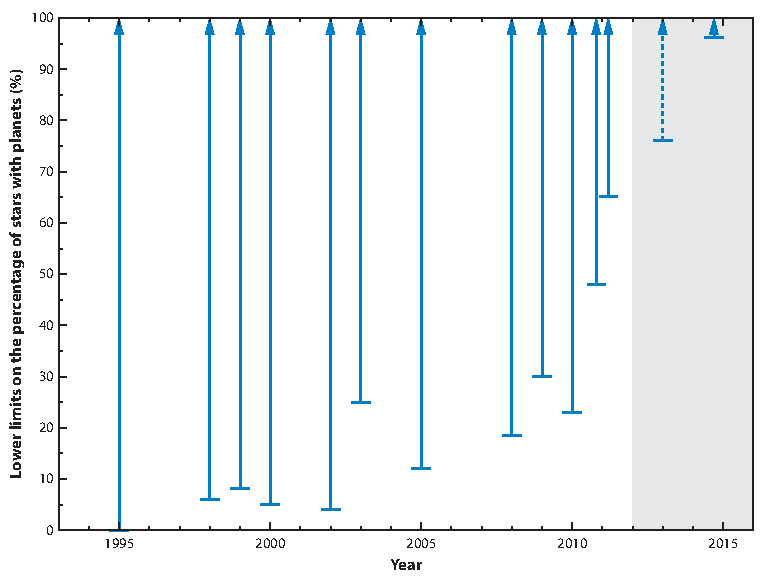
\includegraphics[width=0.9\linewidth]{figures/AnnRevs/AR8.pdf}
	\caption[Fraction of stars with planets]{Lower limits to the fraction of stars with planets as a function of time. Because published values are based on limited ranges in mass or period (\ie, small areas in the parameter space of Figure~\ref{fig:AR9}), they are not estimates of the real fraction of stars with planets but are lower limits. These lower limits have been rising as the durations of surveys increase and detection sensitivity improves. The predicted lower limits at 2013 and 2015, suggesting that 100\% of stars have planets, are based on the trends seen in the past three years and the plausible range over which these trends can be extrapolated}
	\label{fig:AR8}
\end{figure}


%%%%%%%%%%%%%%%%%%%%%%%%%%%%%%%%%%%%%%%%%%
\begin{figure}[!hbt]
	\centering
	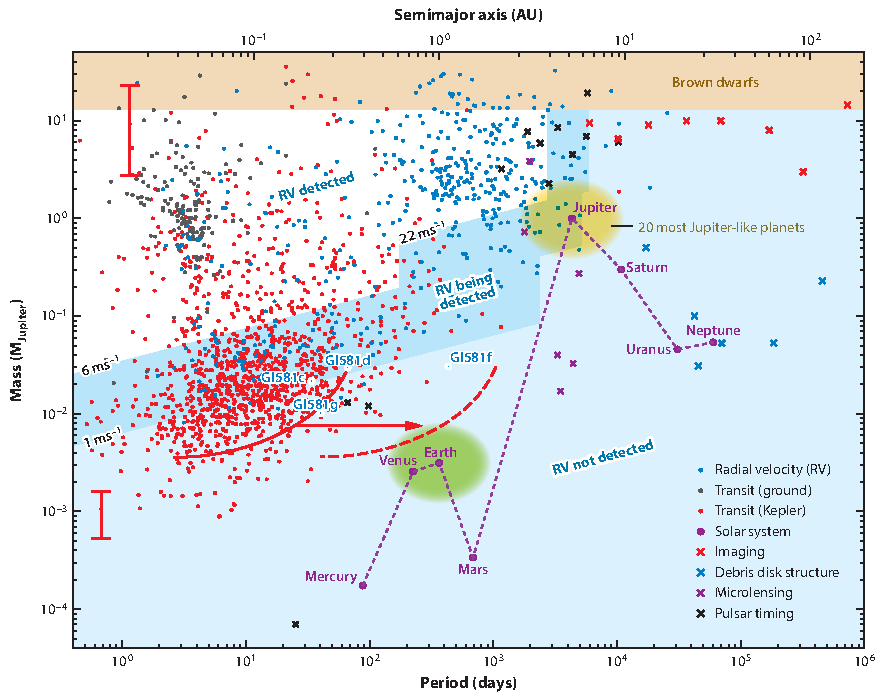
\includegraphics[width=0.9\linewidth]{figures/AnnRevs/AR9.pdf}
	\caption[Exoplanet detection techiques and yeilds]{Our Solar System compared to $\sim$\,1,870 exoplanets detected using various techniques. The region around our planetary system and to the lower right has not been well explored. The red cloud of points in the lower left represents the $\sim$\,1,200 Kepler planet candidates from \citet{Borucki2011}. The other $\sim$\,670 exoplanets were detected by other instruments. After the nominal approximately four-year Kepler mission, the red curve, approximating the limit of the Kepler cloud, will have moved to the dashed red curve. At least a few Earth-mass planets in Earth-like periods around Sun-like stars are expected within the green oval surrounding Earth. If the Sun were removed to some typical distance ($\sim$\,30 light years) and were on the target list of our planet-hunters, it would probably still be listed as having no planets. The yellow oval contains the 20 most Jupiter-like planets, which are plotted separately in Figure~\ref{fig:AR11}. Timothy Bovaird was instrumental in helping to make this figure.}
	\label{fig:AR9}
\end{figure}


Planet detections have technique-dependent limits \citep{Cumming2010}. Figure~\ref{fig:AR9} shows how the eight planets of our Solar System (dashed purple line) compare to the $\sim$\,1,870 exoplanets compiled from six detection techniques listed in the lower right. The estimated masses of the planets are plotted as a function of their orbital periods.

The most important take-home message is: Yes, there are planets around other stars. The second message is that most of the patterns in the data tell us more about instrument sensitivity and survey durations than about the underlying real distribution of planets. Thus, the relatively empty region in the lower right (low mass, long period) appears empty because it has not been well explored. And the blob of dark gray points in the upper left, from ground-based transit searches, is concentrated at high mass and short period because that is where this technique has the highest sensitivity, not because there is a natural concentration of planets there.

The left edge of the red cloud of Kepler points is a real edge due to the underlying distribution of planets and tells us that planets with orbital periods less than a couple of days are rare. The lower right edge of the red cloud (indicated by the red curve) is a result of instrument sensitivity and the duration of observations (only 90 days). At the end of the nominal Kepler mission in 2014, Kepler's region of sensitivity will have extended to the dashed red curve, much closer to the region of Venus- and Earth-like planets.

The background of Figure~\ref{fig:AR9} is color-coded to show the sensitivity of the RV technique to planets orbiting solar-mass stars. The ability of the RV technique to detect planets is 100\% in the white region in the upper left, decreases across the ``RV being detected'' region, and sinks to near 0\% in the ``RV not detected'' region. Thus, in the white ``RV detected'' region, any observed pattern of RV planets (blue dots) is a real pattern and is not due to instrument sensitivity or survey duration. The most obvious pattern is that in the high-mass region (1-10 M$_{Jupiter}$), as periods increase (approaching Jupiter's 12-year period), the number of planets increases dramatically. Thus, Jupiter-mass planets become more numerous as we look in more Jupiter-like orbits.

Because the RV technique is most sensitive in the upper left of Figure~\ref{fig:AR9}, Figure~\ref{fig:AR8} is predominantly telling us about the fraction of stars with massive Jupiter-, Saturn-, Uranus-, and Neptune-sized planets that have been scattered or have migrated from their region of formation (farther from the host star) into a region closer to their host star where they could be detected with the RV technique. However, we are more interested in exoplanets that are more similar to Earth in both mass and period. In Figure~\ref{fig:AR9}, planets indicated by the red Kepler dots are the most similar to Earth in mass. If the fraction of stars with large planets is $\sim$\,100\%, what about the fraction of stars with low-mass rocky planets like Earth\,? Based on extrapolation of RV data, \citet{Howard2010} report ``23\% of stars harbor a close-in Earth-mass planet (ranging from 0.5 to 2.0 Earth masses).'' \citet{Wittenmyer2011} report 17\% for planets with mass less than $\sim$\,13 M$_{Earth}$.

%%%%%%%%%%%%%%%%%%%%%%%%%%%%%%%%%%%%%%%%%%
\begin{figure}[!hbt]
	\centering
	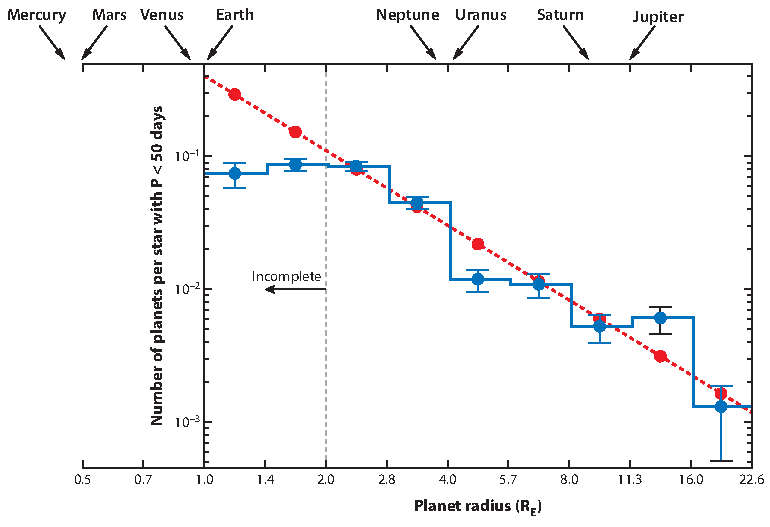
\includegraphics[width=0.9\linewidth]{figures/AnnRevs/AR10.pdf}
	\caption[Kepler results]{Kepler results (as per 2012). The amplitude of the red line tells us that there are many planets close to stars (P < 50 days; for comparison, P$_{Mercury}$ = 88 days). The slope of the red line tells us that there are approximately ten times as many Earth/Venus-sized planets as there are Uranus/Neptune-sized planets and approximately ten times as many Uranus/Neptune-sized planets as there are Jupiter-sized planets. Figure modified from the top panel of Figure~\ref{fig:AR6} in \citet{Howard2012}.}
	\label{fig:AR10}
\end{figure}

Catalogs of exoplanet detections can be found in \citet{Schneider2011} and \citet{Wright2010}. The Kepler planet candidates are from \citet{Borucki2011}. The radii of Kepler candidates have been converted to masses using the average radius-dependent density of the dozen or so least massive exoplanets detected by the transit and radial velocity techniques. Representative uncertainties on this conversion are given in Figure~\ref{fig:AR9} by the size of the vertical error bars on two red points on the far left.

The radii of planets can be extracted from small dips in Kepler's precision photometry of $\sim$\,150,000 stars. Figure~\ref{fig:AR10} is a recent result \citep{Howard2012}. As the fraction of stars with planets approaches its maximum value of 100\% (Figure~\ref{fig:AR8}), this fraction becomes uninformative about the average number of planets per star, which is the y-axis in Figure~\ref{fig:AR10}. The two bins in the region to the left of the dashed gray line (1 < R < 2 R$_{Earth}$) are incomplete because planets that small are harder to detect and need to transit more times for their signal to emerge out of the noise. These incomplete bins were not used to produce the red dashed fit. 

On the left side of Figure~\ref{fig:AR10} notice that the dashed red line crosses R = R$_{Earth}$ at 0.4 planets per star. Because there are many more single-planet stars than multiple-planet systems in the Kepler database, this 0.4 means that $\sim$\,35\% of stars are expected to have planets with radii 0.8 < R < 1.2 R$_{Earth}$ and with orbital periods P < 50 days. That is a large fraction for such a small range of radii and periods. Adding up the values of the red points for the entire range of radii yields the average number of planets (with radii 1 < R < 23 R$_{Earth}$ and P < 50 days) per star: 0.6. When converted to the fraction of stars with a planet, this becomes the 48\% plotted in Figure~\ref{fig:AR8}. Adding up only the values for rocky planets (the three bins with radii 1 < R < 2.8) yields more than 0.5 rocky planets per star. This high frequency within such a small region close to the star (< 0.25 AU) indicates that rocky planets are extremely common.

After Kepler detects more planets with R\,$\approx$\,R$_{Earth}$, if the trend of the red line accurately describes the next smaller bin, the vast majority (perhaps 90\%) of planetary systems may be found to have an Earth-size planet with an orbital period P < 200 days. With Venus's 224-day orbital period and radius R = 0.95 R$_{Earth}$, and Mercury's P = 88 days and R = 0.38 R$_{Earth}$ (too small to detect), such a high observed frequency of close-in exoplanets would make our planetary system unusual for having relatively fewer Earth-sized planets, or having them unusually distant from the host star, or both.

The data collected in Figures \ref{fig:AR8} and \ref{fig:AR9} illustrate that as stars are monitored for longer periods of time, and as we extend our detection sensitivity to Jupiter-like periods, we detect more planets and require less extrapolation to reach the conclusion that $\sim$\,100\% of stars have massive planets. In addition, as we extend our observations to smaller planets (left side of Figure~\ref{fig:AR10}, 0.5 < R < 2 R$_{Earth}$) the numbers increase and again suggest that $\sim$\,100\% of stars have at least one Earth-sized planet.

Other evidence that the fraction of stars with planets is $\sim$\,100\% is that protoplanetary accretion disks are ubiquitous in young star clusters. The observed fraction of young stars with protoplanetary disks approaches 100\% for star-forming regions less than $\sim$\,0.5 million years old \citep{Mamajek2009,Fedele2010}. Also, there are no large planets without a retinue of rocky/icy moons. Many of the moons of Jupiter, Saturn, Uranus, and Neptune are part of miniature planetary systems formed from their planet's miniature accretion disk. ``Planets around every star. Moons around every large planet'' is probably the most reasonable position from which to ponder habitability. Soon we will have detected so many Earth-like planets that our efforts will have to be focused on determining which ones are the most habitable \citep{Horner2010}.

\clearpage

\begin{flushright}
	\textit{If they be inhabited, what a scope for folly;\\if they not be inhabited, what a waste of space.\\
		--- Thomas Carlyle}
\end{flushright}

\section{Circumstellar Habitable Zones}\label{sec:HabitableTemperatures}
Exoplanet research is moving beyond counting planets and plotting their masses and orbital periods. We are beginning to study their temperatures, densities, compositions, tectonic regimes, atmospheric chemistries, and albedos-all factors that can influence habitability. Figure~\ref{fig:AR11} shows that there are several dozen known planets in circumstellar HZs. The least massive are three to five times the mass of Earth. Because the mass of moons seems to scale with the mass of the host planet, the most massive planets in the HZ could harbor habitable moons.

%%%%%%%%%%%%%%%%%%%%%%%%%%%%%%%%%%%%%%%%%%
\begin{sidewaysfigure}[!hbt]
	\centering
	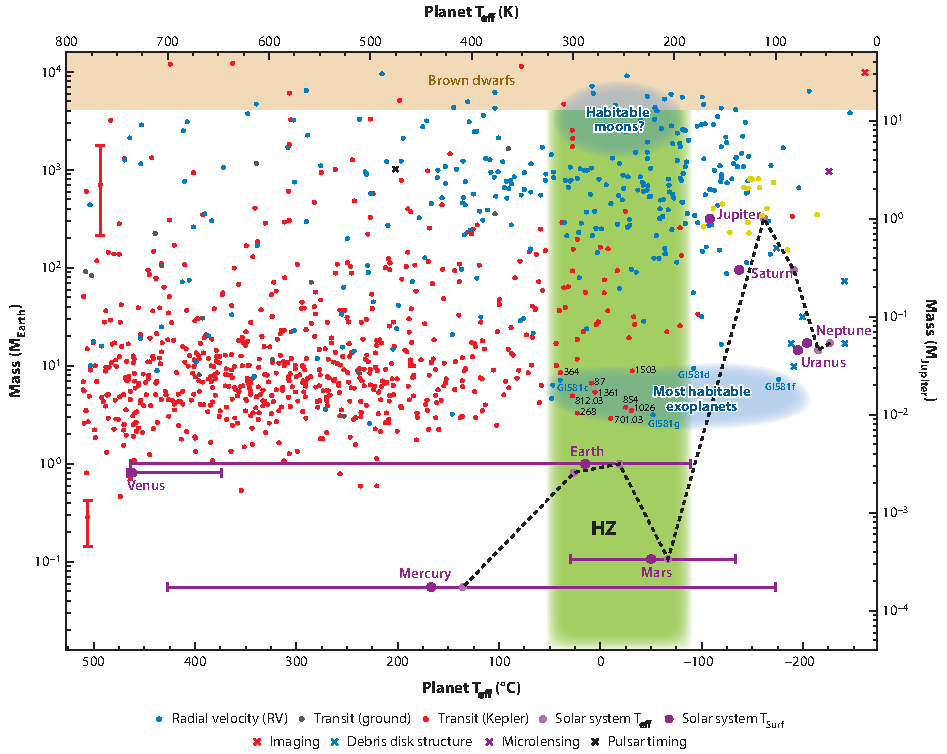
\includegraphics[width=0.65\linewidth]{figures/AnnRevs/AR11.pdf}
	\caption[Planets in the circumstellar habitable zone]{Planet temperatures and the circumstellar habitable zone (HZ). This figure is essentially the same as Figure~\ref{fig:AR9} except we have used our knowledge of the luminosity of the host stars to convert orbital periods into effective temperatures (T$_{effective}$) at the planet's distance from its host. To obtain T$_{effective}$ values for exoplanets and the planets of our Solar System in the same way, we have followed the appendix of \citet[][version 1 only, but using albedo\,=\,0.3, $\varepsilon$\,=\,1, $\beta$\,=\,1]{Borucki2011}. Because we are trying to evaluate the habitability of exoplanets for which we have only T$_{effective}$ values (not actual surface temperatures), we have shifted the habitable temperature range (+122\textcelsius{} to -20\textcelsius{}) by 80\textdegree{} (keeping the 144\textdegree{} width) to be centered on the T$_{effective}$ of Earth. This allows for a more direct comparison of the HZ with exoplanet T$_{effective}$ values and is the simplest way to make a first-order minimal correction for the poorly known extent of exoplanet greenhouse gases and albedos. Because the planets of our Solar System orbit the same star, the dashed lines connecting their (M, T$_{effective}$) coordinates here mirror the dashed lines in Figure~\ref{fig:AR9} connecting their (M, P) coordinates. This is not the case in general. For example, the most Jupiter-like planets (within the yellow oval in Figure~\ref{fig:AR9}) are indicated here with yellow dots. Timothy Bovaird was instrumental in helping to make this figure.}
	\label{fig:AR11}
\end{sidewaysfigure}

For each planet in our Solar System (Figure~\ref{fig:AR11}), notice the difference between the computed effective temperature (T$_{effective}$, small light purple dots) and the actual surface temperatures T$_{Surface}$ (larger purple dots). We have plotted error bars around T$_{Surface}$, indicating the range of surface temperatures on Mercury, Venus, Earth, and Mars. Because $\bigtriangleup${T}{=}T$_{Surface}${-}T$_{effective}$ {>} 0 for all eight planets of our Solar System, all experience some kind of warming.

For Earth we have $\bigtriangleup$T$_{Earth}$ = 33\textdegree, but the thick 90 bar Venutian CO$_{2}$ atmosphere produces $\bigtriangleup$T$_{Venus}$ = 440\textdegree. The variation of $\bigtriangleup$T values within our Solar System is large: 15\textdegree < $\bigtriangleup$T < 440\textdegree, due to differences in albedos and greenhouse gas (CO$_{2}$, H$_{2}$O) column densities. This range gives us an idea of the expected range of exoplanet $\bigtriangleup$Ts that will shift exoplanets to the left in Figure~\ref{fig:AR11}. Thicker atmospheres provide more greenhouse warming and larger $\bigtriangleup$Ts \citep{Marcus2010}. Because we expect $\bigtriangleup$T$_{Super-Earths}$ > $\bigtriangleup$T$_{Earth}$, the shift of the HZ to be centered on the T$_{effective}$ of Earth represents a minimal correction. Thus super-Earths, such as Gl581d just to the right of the HZ, should be considered the best candidates for habitable planets.

A reasonable assumption is that super-Earths (3 < M < 10 M$_{Earth}$) are probably endowed with a mass of greenhouse gases, Mg, proportional to the mass of the planet, M: M$_{g}$ $\sim$\, M. Thus, the column density $\sum$ responsible for greenhouse warming would be $\sum$ $\sim$\, M$_{g}$/surface area $\sim$\, M/R$^{2}$ $\sim$\, R $\sim$\, M$^{1/3}$. With this plausible scaling we would expect the $\bigtriangleup$Ts of super-Earths to be, very roughly, twice as large as the $\bigtriangleup$Ts of our Solar System's planets. Thus, it may be that the half-dozen planets in the middle and left side of the most habitable exoplanets region of the HZ of Figure~\ref{fig:AR11} are greenhouse heated too far to the left to support life.

Gliese 581 is an M star approximately 20 light years away, with a mass M = 0.31 M$_{Sun}$ and $\sim$\,1\% of the Sun's luminosity. Gliese 581's planetary system contains several rocky planets whose habitabilities are being debated \citep{Udry2007,Selsis2007,vonBloh2007,Mayor2009,Wordsworth2011}. The system contains four confirmed planets (Gl581b, -c, -d, -e) and possibly two more unconfirmed planets (Gl581f, -g) \citep{Vogt2010}. With poor signal to noise at the edge of RV sensitivity, the fitted eccentricities can vary between 0 and as much as 0.4. Of the four confirmed planets, Gl581d looks like the best current candidate for being a rocky habitable planet (see also \citep{Kaltenegger2011b}. Its mass is 10$^{{+}4}_{{-}3}$M$_{Earth}$. It receives 35\% less stellar energy than Mars, and its orbital eccentricity is $\sim$\,0. Its period is $\sim$\,66 days and it is tidally locked. It has a radius of $\sim$\,2 REarth, and its surface gravity is approximately twice that of Earth's. Using a global climate model designed for exoplanets, with CO$_{2}$ and H$_{2}$O as greenhouse gases, \citet{Wordsworth2011} find that the range of possible atmospheric pressure is 5-30 bars.

The importance of Gl581 is based on the proximity of its planets to its circumstellar HZ. \citet[][ch 10]{Kasting2012} gives an informed review of the history of the circumstellar HZ and discusses the details of the most cited HZ paper, \citet{Kasting1993}. For details of how the inner and outer limits of the circumstellar HZ are computed, see \citet{Forget1997} and \citet{Abe2011}. The idea of a circumstellar HZ is based on the scenario of surface life kept warm and powered by stellar photons. In the context of the present Earth, this is a reasonable scenario because solar photons control the temperature of the ocean and the top few meters of the continental crust and power most of current life (Figure~\ref{fig:AR4}). But Earth's AHZ may not have been powered by the Sun. If life emerged from a dark hydrothermal vent, vent redox chemistry and the plate tectonic regime that drives it may have more to do with whether life can emerge on a planet than whether the planet is in the circumstellar HZ and has liquid water on its surface. Moving beyond the circumstellar HZ, planets not bound to any star, drifting around between the stars, seem to be the abundant remnants of the gravitational free-for-all in the earliest stages of planet formation in dense star clusters. Using microlensing observations \citet{Sumi2011} report nearly twice as many unbound Jupiters as there are main sequence stars in the galaxy. If there are super-Earths among them with enough hydrogen in their atmospheres \citep{Pierrehumbert2011}, and if life can emerge and persist without photons from a star, then there may be no outer limit to the circumstellar HZ. There may be life-sustaining planets in interstellar space \citep{Stevenson1999}.

\section{Water and Temperature}\label{sec:WaterDel}
Because life as we know it is water-based carbon chemistry, the processes that control the supply of water and carbon to a planet control its habitability. Water is also essential to aid the continual tectonic reworking and erosion that supply key redox gradients and biochemical substrates to sustain habitability (Table \ref{tab:energycurreny}; \citep{Nisbet2007}. \citep{Morbidelli2000} and \citet{Mottl2007} summarize our understanding of the origin of water on Earth. D/H ratios \citep{Robert2001} and much other evidence suggest that the sources of terrestrial water were hydrous bodies such as carbonaceous chondrites (5\%–20\% water) from the outer part of the main asteroid belt. An alternative wet accretion model has between one and three oceans of water accreting with the planetary embryos that formed the bulk Earth \citep{Drake2002, Drake2005}. A third possibility discussed by \citet{Mottl2007} is the acquisition of hydrogen and water directly from the solar nebula by adsorption onto accreting material and dissolution into a magma ocean.

Because variations in temperature and water content are the two most important variables in delimiting the habitability of Earth, they should be the basis of any classification scheme for the habitability of planets. The green circumstellar HZ in Figure~\ref{fig:AR11} is based on effective temperature computed from stellar type and semimajor axis. To obtain more accurate surface temperatures, we need to know more about planetary greenhouse gas content and albedos. The amount of water on a rocky planet can depend on the C/O ratio of the star (because C/O controls the amount of water in the protoplanetary disk), but like T$_{Surf}$, water content depends on many variables. Numerical simulations that take into account the notionally most important parameters indicate that water content on a terrestrial planet can vary typically by factors of a few \citep{Raymond2007} and probably much more (perhaps an order of magnitude) when more parameters are allowed to vary. Variations in water supply are caused by variations in the number of impacts with water-rich planetesimals. The number of impacts is a function of planetary position (proximity to the snowline) and planetary mass (to gravitationally focus the impactors). Impacts also depend on the mass, eccentricity, and orbital evolution of the Jupiter analog in the system (if there is one) \citep{Levison2003,OBrien2006}.

\begin{table}[tbh]
	\centering
	\caption{Planet classification according to water content}
	\resizebox{\textwidth}{!}{
	\begin{tabular}{@{}lcc@{}}
		\toprule
		{Name}     & {\% surface} & {Features}\\ 
		   & {liquid water} & \\ \midrule
		Ocean planet      &  $\sim$\,100\%                           & Hydrothermal vents, little erosion \citep{Kuchner2003,Leger2004}\\
		Earth-like planet & 1\%-99\%                         & Continental and oceanic crust, surface erosion, fresh water\\
		Desert planet     &  $\sim$\,0\%                             & Wider habitable zones\,?  \citep{Abe2011}\\ \bottomrule
	\end{tabular}
	}
		\label{tab:planetclassification}
\end{table}

\begin{table}[tbh]
\caption{Planet classification according to water content}

\label{tab:planetclassification2}
\centering
\begin{footnotesize}
\rowcolors{3}{tableShade}{white} %% start alternating shades from 3rd row
\begin{tabular}{cll}
\toprule
\hiderowcolors 
\tabhead{Name} & \tabhead{\% surface} & \tabhead{Features}\\
 & \tabhead{liquid water} & \\
\midrule
\showrowcolors
Ocean planet      &  $\sim$\,100\%                           & Hydrothermal vents, little erosion \citep{Kuchner2003,Leger2004}\\
		Earth-like planet & 1\%-99\%                         & Continental and oceanic crust, surface erosion, fresh water\\
		Desert planet     &  $\sim$\,0\%                             & Wider habitable zones\,?  \citep{Abe2011}\\ \bottomrule
\end{tabular}
\end{footnotesize}
\end{table}

Another complication is that Earth may have acquired far more water during its formation than exists in its ocean and mantle today \citep{Abe2000}. Variations in the ability of a planet to hold onto the supplied water depend on planetary mass, temperature (through thermally induced hydrodynamic escape), atmosphere, the amount of collisional erosion \citep{Genda2005,ONeill2008}, and the degree of differentiation of the impacting planetesimals. In the first few million years, $^{26}$Al (half-life 0.7 million years) provides much of the radiogenic heat (in addition to the heat of accretion) responsible for the density segregation of planetesimals, exposing water on the outside while sequestering iron on the inside \citep{Grimm1993,Hester2005}. Importantly, the $^{26}$Al content of a protoplanetary disk can vary by several orders of magnitude since it depends on how close the disk is to the closest supernovae produced by the largest stars in the birth cluster \citep{Bizzarro2004,Gaidos2009,Gilmour2009,Adams2010}. Because of the large variation possible in the water content of rocky planets, it makes sense to classify them by water content and by the phase of that water (solid, liquid, or gas) (see Table \ref{tab:planetclassification}). 


Ocean, Earth-like, and desert planets will each have low-, moderate-, and high-temperature versions. For example, a low-temperature ocean planet will be covered with ice (Europa-like), possibly because it is too small to maintain ongoing volcanism, or too poor in the four long-lived radiogenic isotopes to recover from episodes analogous to snowball Earth \citep{Hoffman2002}. A high-temperature version of an ocean planet would be a steam planet. Desert planets, low in H$_{2}$O owing to a small amount of radial mixing of material beyond the snowline, would also be low in carbon. Low carbon could also be a factor limiting the habitability of planets orbiting stars with low C/O ratios. See \citet{Bond2010} and \citet{Delgado-Mena2010} for a discussion of how stellar variation in C/O and Mg/Si can affect the mineralogy and habitability of rocky planets. For example, they find that stars with C/O > 0.8 will host reduced carbide planets with little water.

\clearpage
\section{The Galactic Habitable Zone}\label{sec:GHZ}

Life is embedded in a hierarchy of supporting environments that provide the requirements for habitability. Estimation of a circumstellar HZ assumes the presence of a star and a planet and addresses the question, Where can the planet be located such that its surface is at the right temperature for life\,? The galactic HZ is a similar idea but on a much larger scale: Given an 11-billion-year-old galaxy, where can you find a star, a rocky planet, and clement conditions that last long enough to maintain life\,? The idea of a galactic HZ was intimated by  \citet{Lem1986}, clearly articulated by \citet{Gonzalez2001}, extended and more carefully quantified by \cite{Lineweaver2004} (Figure~\ref{fig:AR12}), and refined spatially to individual stars in a Monte Carlo simulation by \citet{Gowanlock2011} \citep[see however,][]{Prantzos2008}. Stars in our galaxy are not distributed uniformly in either space or time, nor do they all have enough metallicity (elements excluding H, He) to accrete rocky planets. And some are dangerously close to supernovae that disrupt habitability. \citet{Lineweaver2004} mapped the distribution in space and time of four prerequisites for complex life: the presence of a host star, enough heavy elements to form terrestrial planets, sufficient time for biological evolution ($\sim$\,4 billion years), and an environment free of life-extinguishing supernovae. We identified the galactic HZ as an annular region between seven and nine kiloparsecs from the galactic center that widens with time and is composed of stars that formed between eight and four billion years ago. Similar to the boundaries of the circumstellar HZ, these limits are not sharp, but do indicate where the potential for complex (= 4 billion years old) life may be the highest. This galactic HZ yields an age distribution for the complex life that may inhabit our galaxy: 75\% of the stars in the galactic HZ are older than the Sun.

%%%%%%%%%%%%%%%%%%%%%%%%%%%%%%%%%%%%%%%%%%
\begin{figure}[!hbt]
	\centering
	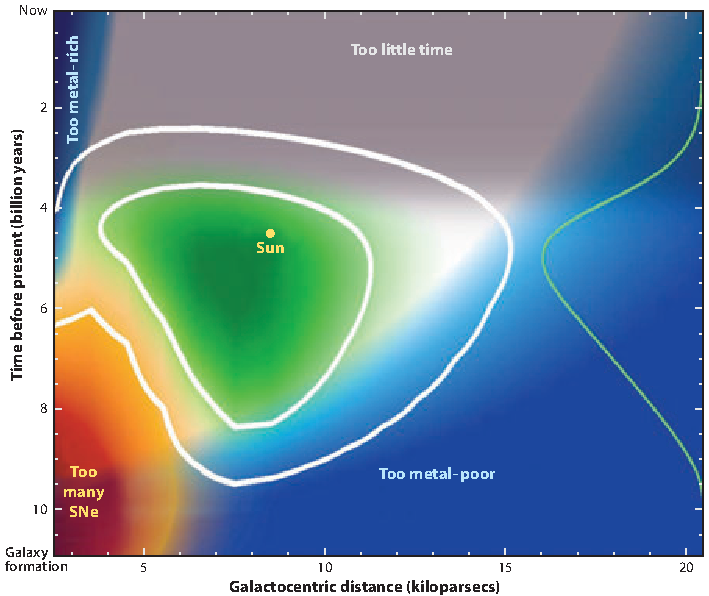
\includegraphics[width=1\linewidth]{figures/AnnRevs/AR12.pdf}
	\caption[Galactic habitable zone]{Galactic habitable zone (HZ) of our Milky Way Galaxy from \citet{Lineweaver2004}. ``Too many SNe'' indicates the region where the supernovae (SNe) rate is probably too high to be compatible with the evolution of life.}
	\label{fig:AR12}
\end{figure}

Stars in our galaxy are not distributed uniformly in either space or time, nor do they all have enough metallicity (elements excluding H, He) to accrete rocky planets. And some are dangerously close to supernovae that disrupt habitability. \citet{Lineweaver2004} mapped the distribution in space and time of four prerequisites for complex life: the presence of a host star, enough heavy elements to form terrestrial planets, sufficient time for biological evolution ($\sim$\,4 billion years), and an environment free of life-extinguishing supernovae. We identified the galactic HZ as an annular region between seven and nine kiloparsecs from the galactic center that widens with time and is composed of stars that formed between eight and four billion years ago. Similar to the boundaries of the circumstellar HZ, these limits are not sharp, but do indicate where the potential for complex (= 4 billion years old) life may be the highest. This galactic HZ yields an age distribution for the complex life that may inhabit our galaxy: 75\% of the stars in the galactic HZ are older than the Sun.

One can extend the concept of HZ beyond the galaxy to the universe. For example, a cosmic temporal HZ can be constructed from the age distribution of terrestrial planets in the universe \citep{Lineweaver2001}. There are times that are habitable and times that are not. In the first two to three billion years after the big bang, there were no terrestrial planets because there was not enough condensable material to make them. There are also many other features of our universe that play a role in its habitability. These are discussed insightfully elsewhere \citep{Dicke1961,Carter1974,Barrow1988,Bostrom2002,Carroll2006,Barrow2006}.

Following \citeauthor{Lovelock1965}'s \citeyear{Lovelock1965} idea that the simultaneous presence of oxygen and reduced gases (\eg~CH$_{4}$, H$_{2}$) is unlikely without life, \citet{Sagan1993} analyzed a spectrum of Earth taken by the Galileo probe, searching for signatures of life. They concluded that the large amount of O$_{2}$ and the simultaneous trace amounts of CH4 are strongly suggestive of biology. This has been a model of how we might be able to remotely detect life elsewhere \citep{Leger1999}. However, oxygen can be produced abiotically by photolysis of water with subsequent hydrogen escape and photolysis of CO$_{2}$ with subsequent burial of carbon. The future search for extraterrestrial life will rely on our improved ability to understand and spectrally characterize the abiotic and potentially biotic contributions to atmospheric chemical disequilibria \citep{Kasting2009,Krissansen-Totton2016,Seager2010,Vazquez2010,Kaltenegger2011b}.

The study of habitability, \textit{habitology}, is a new, cross-disciplinary synthesis of facts and theory from Earth and planetary sciences, biology, and astronomy. As new data come streaming in from these disparate disciplines, the preliminary steps of their integration is exhilarating and confusing. We can only find out who we are and how we fit into the universe by studying and interpreting these data with the goal of finding other life-forms. Our search for extraterrestrial life is a search for ourselves and our place in the universe. If we cannot find extraterrestrial life-forms that fit our definition of life, perhaps we will have to broaden our definition until we do. Even if we fail to find life elsewhere, we will soon find the closest uninhabited habitable planet. That will be crucial, sooner or later, for our survival as a species.
\chapter{The Biology of Habitability}\label{ch:biologicalhab}
This chapter was published as
\begin{description}
	\item \fullcite{Chopra2016}
\end{description}
\bigskip
\section*{Abstract}
The prerequisites and ingredients for life seem to be abundantly available in the universe. However, the universe does not seem to be teeming with life. The most common explanation for this is a low probability for the emergence of life (an emergence bottleneck), notionally due to the intricacies of the molecular recipe. Here, we present an alternative Gaian bottleneck explanation where the emergence of life could be much more common than its long term persistence. If life emerges on a planet, it only rarely evolves quickly enough to regulate greenhouse gases and albedo, thereby maintaining surface temperatures compatible with liquid water and habitability. Such a Gaian bottleneck suggests that (i) extinction is the cosmic default for most life that has ever emerged on the surfaces of wet rocky planets in the universe and (ii) rocky planets need to be inhabited to remain habitable.
In the Gaian bottleneck model, the maintenance of planetary habitability is a property more associated with an unusually rapid evolution of biological regulation of surface volatiles, than with the luminosity and distance to the host star.  Liquid water on the surface of a planet (particularly old planets) would then not just be a prerequisite for life, but a plausible biosignature.
\clearpage

\section{Where is everybody?}

We see no evidence that our galaxy has been colonized by an advanced technological civilization.
Archaeological excavations have not unearthed alien spaceships, and the optical and radio searches for extraterrestrial intelligence have not been successful \citep{Tarter2001}. 
If one assumes that, once life emerges it evolves towards intelligence and technological civilizations, we are faced with Fermi's paradox: Where is everybody? (\citet{Webb2002,Cirkovic2009}; but also see \citet{Gray2015} and \citet{Ward2000}).
To put this information in context, \citet{Hanson1998} introduced the concept of a Great Filter, describing the possible bottlenecks in the assumed progression from molecular chemistry to life, from life to intelligence, and from intelligence to galactic colonization.
If the emergence of life is a rare and difficult process, then an emergence bottleneck could resolve Fermi's paradox.
However, if technological civilizations inevitably destroy themselves, this self-destruction bottleneck could also resolve Fermi's paradox.

\citet{Bostrom2008} argued that the Great Filter is a valuable tool for assessing existential risks to humanity. If the biggest barrier in the Great Filter is the emergence bottleneck, then we will find no independently evolved life on Mars, and the apparent absence of 
advanced technological civilizations in our galaxy is because life's emergence is difficult and rare. %Conway Morris 2005 
In this case, humanity has already survived the biggest threat to its continued existence; the biggest bottleneck is behind us and we can relax.
However, if we find life on Mars that has evolved independently of life on Earth, this would be strong evidence that there is no
emergence bottleneck. If we find such life, Bostrom argues that the biggest bottleneck -- the self-destruction bottleneck -- would then be in front of us. This would be ``by far the worst news ever printed on a newspaper cover.''
As a plausible alternative to such catastrophic logic, we introduce the concept of a Gaian bottleneck, a bottleneck that life on Earth has already passed through. 
If such a bottleneck exists, the discovery of \textit{extant}, independently evolved martian life might be bad news, but the discovery of \textit{extinct} independently evolved martian life, would not be.

In the standard view, the decrease in bombardment rate  from $\sim$4.5 to $\sim$3.8 Gya is associated with making Earth more clement and thus enabling life to emerge and persist \citep{Maher1988}.
In contrast to this view, we postulate  
a Gaian bottleneck model in which early life (on Earth and elsewhere) is not just a passive passenger, but comes under strong selection pressure
to actively modify and regulate its environment. 
The emergence of life's abilities to modify its environment and regulate initially abiotic feedback mechanisms (what we call Gaian regulation)
could be the most significant factor responsible for life's persistence on Earth.

This highlights an important difference between physics-based estimates of habitability
and the more unpredictable patterns of biological evolution 
on the highly unstable surface environments of young terrestrial planets. For example, bombardment rates inevitably decrease in the circumstellar habitable zones (CHZ) of stars, but  the time scales for the evolution of Gaian regulation is probably unpredictable and would not inevitably evolve rapidly (or at all). Thus, if there is anything special about what happened on Earth  to allow life to persist here, it might have less to do with the
decreasing bombardment rate in the Hadean, or special chemical ingredients, or sources of free energy, or even a rare recipe for the emergence of life.  The existence of life on Earth today might have more to do with the unusually rapid biological evolution of effective niche construction and Gaian regulation
in the first billion years. Habitability and habitable zones would then not only be a passive abiotic property of stellar and planetary physics and chemistry 
(such as stellar luminosity, initial water content, and decreasing bombardment rate) 
but would also be a result of early life's ability to influence initially abiotic geochemical cycles and turn them into the life-mediated biogeochemical cycles 
that we are familiar with on the current Earth \citep{Lenton1998,Lenton2004,Schneider2004,Falkowski2008,Kump2009}. Without rapid evolution of Gaian regulation, early extinction would be the most common fate of planetary life. Even if the emergence of life is a common feature of wet rocky planets throughout the universe, the Gaian bottleneck model suggests that inhabited Earth-like planets would be rare.
%%%%%%%%%%%%%%%%%%%%%%%%%%%%%%%%%%%%%%%%%%

\section{Is abiogenesis rare?}
\subsection{Possible physics and chemistry based bottlenecks}
\label{sec:EmergenceBottleneck}

\subsubsection{No stellar bottleneck.  No wet-rocky-planet bottleneck. Sun-like stars and Earth-like planets are common.}
If our Sun were the most uranium-rich star in the galaxy, and if life on Earth were uranium-based (instead of carbon-based), then we would have good reason 
to believe that life (either its emergence, persistence, or both) requires a rare kind of uranium-rich host star. 
However, we have been unable to identify any significant differences between the Sun and other stars that could plausibly be connected with an
increased probability of abiogenesis. 
Sun-like stars are common in the universe  \citep{Robles2008}.
Thus, there seems to be no stellar bottleneck responsible for reducing the probability for the emergence of life.

Over the past decade, estimates for the frequency of rocky planets in, or near, the CHZ have increased \citep{Howard2012,Lineweaver2012AnnRev,Petigura2013,Bovaird2013,Fressin2013,Marcy2014,Bovaird2015,Burke2015}.
Rocky planets in the CHZ are likely to be a common outcome of planetary formation.
This result is supported by observational, theoretical, and computational models of rocky planet formation in which gas-rich protoplanetary disks evolve into dust disks
in which planetesimals form and undergo oligarchic growth into planetary embryos as they
differentiate into iron-nickel-rich cores, silicate mantles, and crusts dominated by incompatible lithophiles \citep{Morbidelli2012,Elkins-Tanton2012,Chambers2014,Hardy2015}. Models and observations suggest that this sequence -- the formation of terrestrial planets -- is not a rare occurrence that needs special initial conditions. There seems to be no rocky-planet-in-the-CHZ bottleneck responsible for reducing the probability for the emergence of life.

\subsubsection{No elemental or molecular ingredient bottleneck.}

Life on Earth is made of hydrogen, oxygen, carbon, nitrogen, sulfur, and phosphorus: ``HOCNSP'' \citep{Chopra2010}. HOCNPS are among the most abundant atoms in the universe \citep{Pace2001,Lodders2009a,Lineweaver2012}. Since the elemental ingredients for life are the most common elements in the universe, it is not surprising that the molecular ingredients of life are also common.

Of the elements in the universe that form molecules, water (H$_{2}$O) is the combination of the first and second most abundant elements. 
Water should be a common feature of rocky planets \citep{Raymond2004,Raymond2007,Elkins-Tanton2012}.
Radial mixing during the epoch of oligarchic growth ensures that some water-rich materials from beyond the snowline are injected into the more water-poor material
of the feeding zones of rocky planets in the CHZ.
Thus, it is likely that Mars and Venus both started out, like Earth, hot from accretional energy and impacts, and wet from impacts of large
hydrous (5\% - 20\% water) asteroids from the outer asteroid belt \citep{Morbidelli2000,Morbidelli2012} and other ``wet'' accretionary material \citep{Drake2002,Drake2005}.
Terrestrial planets in other planetary systems are also likely to start with variable, non-negligible amounts of water.

Current terrestrial life is built of monomers such as amino acids, fatty acids,
sugars, and nitrogenous bases. Amino acids link together to form proteins; fatty acids link to form lipids; sugars link to form carbohydrates; 
and nitrogenous bases combine with sugar and phosphate to make nucleotide monomers, which link to form RNA/DNA \citep{Lineweaver2012}. 
Thus, life on Earth emerged when available monomers linked together to make polymers. 
Amino acids and other organic monomers fall from the skies in carbonaceous chondrites.
We have no reason to believe that the availability of these monomers is somehow unique to Earth or the Solar System.
The flux of such organics was particularly high during the first billion years of the formation of Earth, and we have no reason to believe
that this will not be the case during the formation of terrestrial planets in other planetary systems.
The assortment of organic compounds found in carbonaceous chondrites
and the probable universality of early heavy meteoritic bombardments indicate that new planetary systems should also be
supplied with organic ingredients and be conducive to the synthesis of prebiotic molecules  \citep{Ehrenfreund2000,Herbst2009,Tielens2013}. We expect all the ingredients of life as we know it (HOCNPS, water, amino acids, sugars, nucleic acids, HCN, and other organics)
to be present and available on wet rocky planets throughout the universe.  An ingredient bottleneck seems implausible.

\subsubsection{No free energy bottleneck since photon and chemical redox based energy sources are common.}

Life (here and elsewhere) needs to do something for a living \citep{Conrad2001,Nealson2013}.
This living depends on extracting free energy from an environment out of thermodynamic equilibrium \citep{Branscomb2013}. 
This extraction is based on catalyzing redox reactions or absorbing photons \citep{Kleidon2011}.
The interiors of rocky planets throughout the universe are denser and hotter than their surfaces.
Thus, thermal gradients, density gradients, and the fluid flows they drive, set up redox potentials that can be exploited \citep{Nisbet2014}.
The environmental factors that enabled abiogenesis on Earth, such as the geochemical  disequilibria between rocks, minerals, aqueous species, and gases, are likely to be ubiquitous 
on wet rocky planets throughout the universe. 
In addition, for planets in the CHZ, fusion in a nearby star shines $\sim$6000 K photons onto $\sim$300 K surfaces and enables
metabolisms based on photon capture \citep{Lineweaver2008a,Annila2008}.

\subsubsection{Recipe bottleneck\,? How ubiquitous are Abiogenesis Habitable Zones?}
\label{sec:recipe}

With the absence of bottlenecks associated with stars, planets, ingredients, and sources of free energy, the only other factor that could produce an
emergence bottleneck would be ``recipe.'' While we do not know the specifics of the prebiotic chemistry and geochemical environments necessary for life to emerge \citep[\eg,][]{Orgel1998,Stueken2013}, the view that life will emerge with high probability on Earth-like planets is shared by many scientists.
\citet{Darwin1871} speculated that the environment, ingredients, and energy sources needed for the origin of life could be common, when he wrote about life emerging in...

\begin{quotation}
	...some warm little pond with all sort of ammonia and phosphoric salts, light, heat, electricity present, that a protein compound was chemically formed, ready to undergo
	still more complex changes.
\end{quotation}
\citet{DeDuve1995} has been a more recent proponent of the view that the emergence of life is a cosmic imperative:
\begin{quotation}
	Life is either a reproducible, almost commonplace manifestation of matter, given certain conditions, or a miracle. Too many steps are involved to allow for something in between.
\end{quotation}
Discarding miracles, de Duve leaves us with life as an ``almost commonplace manifestation of matter.''
As far as we know, Darwin's warm little pond, or deDuve's ``certain conditions'' are common on Earth-like planets and may be sufficient for the emergence of life.
Biota throughout the universe would emerge from chemistry through proto-biotic molecular evolution \citep[\eg,][]{Eigen1992,Eschenmoser1996,Orgel1998,Ward2000,Martin2007,Russell2013}.
%However, ``..we don't get Darwinian behaviour out of chemical systems spontaneously, or even when we try.'' (Benner 2010).

There is some tension between this conclusion and  the inability of synthetic biologists to produce life, despite having access to a wide variety of ingredients, environmental set ups, and energy sources.
Plausible explanations for this tension include:
(1) there is an emergence bottleneck due to a convoluted recipe whose requirements only rarely occur naturally.
Or (2) there is no emergence bottleneck -- the recipe for life is simple -- but we are not as imaginative or as resourceful as nature, so we have not replicated the recipe in the relatively short time we have been investigating the origin of life.

We conclude that the idea of an emergence bottleneck is still plausible. 
However, the evidence for it is getting weaker as we find out more about the proto-biotic molecular evolution that led to the emergence of life on Earth
\citep[\eg,][]{Benner2013,England2013,Nisbet2014,Sousa2014}.
This weakness provides motivation for alternative explanations for the apparent paucity of life in the universe.
The Gaian bottleneck hypothesis is one such alternative.

As we learn more about the origin of life, we can begin to define an abiogenesis habitable zone (AHZ) where the requirements for life's emergence are met. 
Many initially wet rocky planets in the CHZ may possess the necessary and sufficient conditions to get life started  (``AHZ'' in Figure \ref{fig:AHZ}). The habitability requirements for the origin of life may be substantially different from, and more specific than, the requirements to maintain life on a planet  (as in the difference between the need to have a spark plug to start an engine and a radiator to keep it from overheating). In Figure \ref{fig:AHZ}, we have assumed that the AHZ is not necessarily a subset of currently inhabited planetary environments.
%%%%%%%%%%%%%%%%%%%%%%%%%%%%%%%%%%%%%%%%%%
\begin{figure}[!ht]
	\centering
	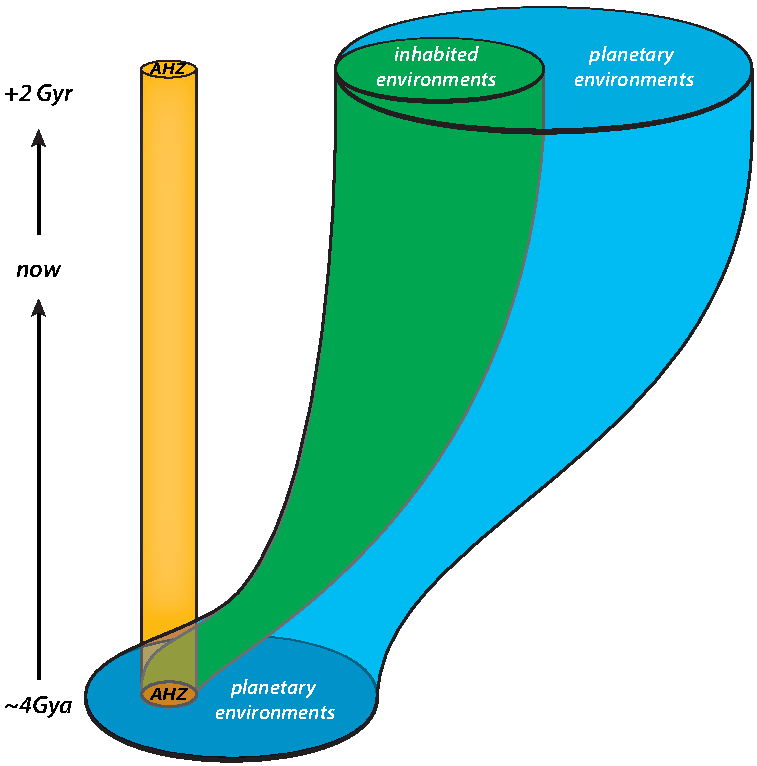
\includegraphics[width=0.6\linewidth]{figures/AHZ.pdf}
	\caption[Abiogenesis Habitable Zone]{The conditions needed for the origin of life are in the Abiogenesis Habitable Zone  or ``AHZ.''
		Inhabited environments (green) are a subset of planetary environments (blue).
		Both of these can change with time.
		The AHZ conditions are probably narrower than the broader conditions to which life can now adapt (``inhabited environments'').
		Through its management of the greenhouse and its partitioning of reductants and oxidants, the activity of life increases the range of inhabited environments \citep{Nisbet2007}.
		Hence, the green cylinder emerges out of the AHZ and gets broader with time.
		More specific reasons for this broadening include (1) the evolution of increasingly efficient catalytic enzymes offering tighter control over reaction rates, 
		(2) the ability of new enzymes to access the energy from different redox pairs providing larger $|\Delta G|$ values \citep{Nealson1999}, and
		(3) the evolution of ecosystems \citep{Smith2015}, global level niche construction, and global biogeochemical feedback cycles (see Section \ref{sec:biofeedbacks}) which we refer to as 
		the ``evolution of Gaian regulation of the biosphere.''
		%Life evolved spores to survive dry conditions, anti-freeze to survive at low temperature and salt pumps to survive at high salinity. 
	}
	\label{fig:AHZ}
\end{figure}

\subsection{Emergence Bottlenecks vs Gaian Bottlenecks}
An emergence bottleneck is illustrated in Figure \ref{fig:EmergenceBottleneck}.
The left panel  shows a hypothetical planet with non-evolving planetary conditions.
The right panel shows a more plausible planet which initially had some habitable regions but, through volatile evolution or other
transient factors, lost its surface water and evolved away from habitable conditions (\eg, a runaway greenhouse or runaway glaciated planet).
Without significant abiotic negative feedback mechanisms, the surface environments of initially wet rocky planets are volatile and change rapidly
without any tendency to maintain the habitability that they may have temporarily possessed as their early unstable surface temperatures transited
through habitable conditions (Figure \ref{fig:GaianHZ} C).
%%%%%%%%%%%%%%%%%%%%%%%%%%%%%%%%%%%%%%%%%%
\begin{figure}[!t]
	\centering
	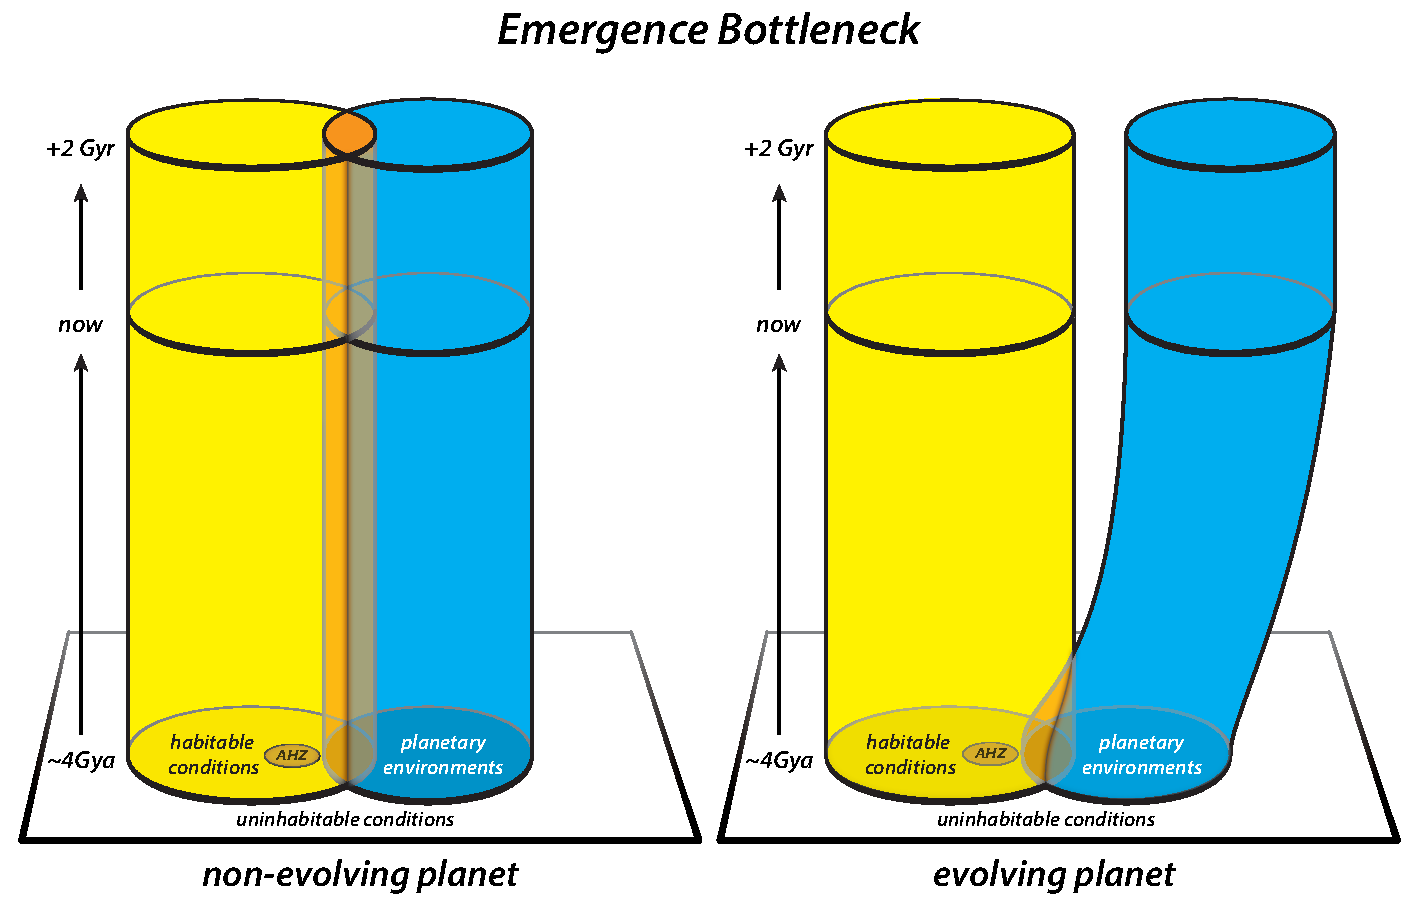
\includegraphics[width=0.9\linewidth]{figures/EmergenceBottleneck.pdf}
	\caption[Emergence Bottleneck]{Emergence Bottleneck: planets on which life does not get started.
		Here, we show habitable conditions (yellow) and planetary environments (blue), from the time of planet formation at the bottom to $\sim$6 billion years later at the top.
		Life will not emerge on either of these planets since their initial planetary environments do not overlap with the Abiogenesis Habitable Zone (AHZ) where life could get started.
		Both of these planets are initially habitable since their environments overlap with habitable conditions. \textit{Left panel:} In this unrealistic, non-evolving model, planetary environments do not change with time. Habitable regions remain uninhabited because life does not get started. 
		Such planets are uninhabited but remain habitable. \textit{Right panel:}  Parts of this evolving planet were habitable, but life does not emerge. The planet undergoes abiotic evolution and moves quickly away from habitability.
		We argue (Section \ref{sec:awayfromhabitability}) that evolution away from habitability is probably the default for initially wet rocky planets.
		We would find such planets to be uninhabited (and if older than $\sim$1 Gyr, uninhabitable) -- consistent with the idea that a planet has to be inhabited to remain habitable.}
	\label{fig:EmergenceBottleneck}
\end{figure}
%%%%%%%%%%%%%%%%%%%%%%%%%%%%%%%%%%%%%%%%%%
If there is no emergence bottleneck (Figure \ref{fig:GaianBottleneck}), typical wet rocky planets have initial conditions compatible with the emergence of life (AHZ). We postulate that almost all initially wet rocky planets on which life emerges (left panel of Figure \ref{fig:GaianBottleneck}) quickly evolve like the abiotic planets  represented in the right panel of Figure \ref{fig:EmergenceBottleneck}. This unregulated evolution of planetary environments away from habitable conditions constrains the duration of life's existence on the planet. We call this early extinction of almost all life that ever emerges the \textit{Gaian bottleneck}. In rare cases (for example on Earth), life will be able to evolve quickly enough to begin to regulate surface volatiles through the modification of abiotic feedbacks (right panel of Figure \ref{fig:GaianBottleneck}). The potentially relevant feedbacks involved in such early Gaian regulation are illustrated in Figure \ref{fig:feedbacks} and discussed in Table~\ref{tab:feedbacks} and Section \ref{sec:biofeedbacks}.
%%%%%%%%%%%%%%%%%%%%%%%%%%%%%%%%%%%%%%%%%%
\begin{figure*}[!t]
	\centering
	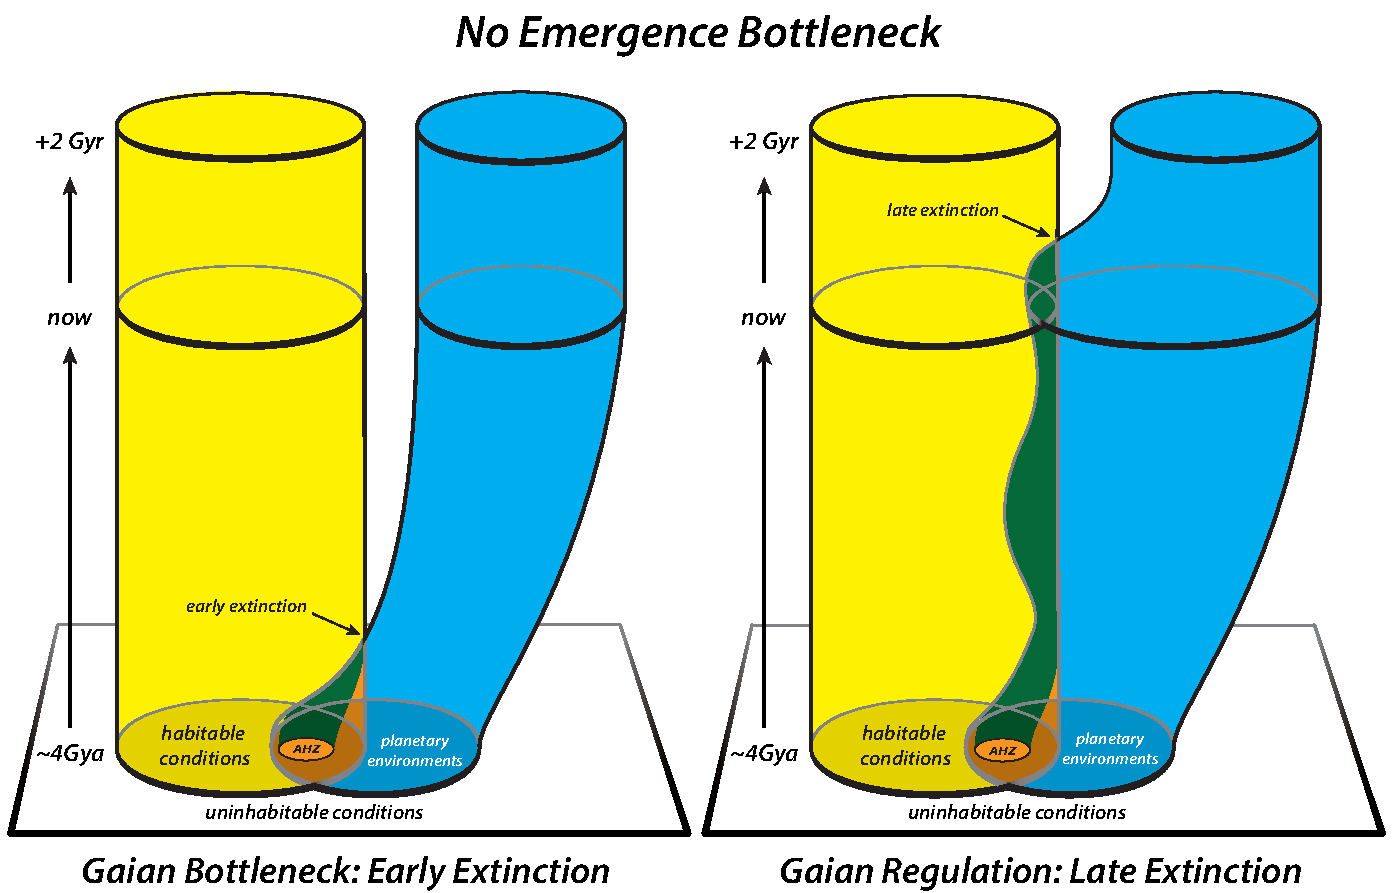
\includegraphics[width=0.9\linewidth]{figures/GaianRegulation.pdf}
	\caption[Gaian Regulation]{The Abiogenesis Habitable Zone may be a very common subset of the environments of rocky planets that are wet during their first billion years.
		As in the left panel of Figure \ref{fig:EmergenceBottleneck}, we assume that these planets are unregulated by any abiotic negative feedbacks and have no tendency to maintain habitability.
		We assume that life gets started on both these planets, so there is no ``emergence bottleneck'' (Section \ref{sec:EmergenceBottleneck}) as there was in
		Figure \ref{fig:EmergenceBottleneck}.
		\textit{Left panel:} Life is unable to evolve rapidly enough to control runaway positive feedbacks.
		Gaian regulation does not emerge fast enough to maintain habitability. 
		Thus, we have a ``Gaian bottleneck.'' We propose that most wet rocky planets are of this kind.
		\textit{Right panel:} In rare cases (as on Earth), Gaian regulation evolves fast enough to make it through the Gaian bottleneck and
		keep at least part of the planet habitable for billions of years. 
		Biospheric regulation maintains the habitability of the planet until $\sim$5 Gyr after formation, at which time, increasing stellar luminosity and loss of water
		cause life to go extinct.
		Extinction happens in both panels but much later in the right panel.
		This figure illustrates our hypothesis that the emergence and rapid extinction of life may be quite common (left) but that the emergence of life, followed by the evolution of Gaian regulation and the long term persistence of life, could be quite rare (right).}
	\label{fig:GaianBottleneck}
\end{figure*}

\section{Early extinction in the first billion years}
\subsection{Bombardment and impact frustration}

During the late phases of Earth's accretion ($\sim$4.5 to $\sim$4.0 Gya), episodes of cold ``Norse ice-hell'' were punctuated by
brief periods of hot inferno with magma oceans \citep{Nisbet2002,Elkins-Tanton2008}. 
Frequent, large, random impacts produced wide-ranging, unstable temperatures.
The largest impacts were so large that any life that did emerge during the transitory habitable periods was probably bombarded into extinction.
These early bombardment-induced extinctions have been called the impact frustration of life \citep{Maher1988,Sleep1989,Sleep2014,Davies2005,Marchi2014}.
The early heavy bombardment of Earth decreased by more than $\sim$13 orders of magnitude during this period (\citet{Bland2005,Koberl2006} 
Figure \ref{fig:GaianHZ} A).
As the rate of planetary accretion slowed, the impact rate and the size of the largest impactors decreased.
Habitable conditions became, at least fleetingly, more available for life \citep{Abramov2009,Abramov2013}. Impact heating may have provided strong selection pressure on early life to evolve into deep environments to survive thermal perturbations \citep{Sleep1989,Nisbet2001,Mat2008}.

We have no reason to believe that these processes are specific to Earth or to our Solar System. The surfaces of Earth-sized rocky planets will undergo an early heavy bombardment that produces severe intermittent temperature pulses. A decreasing bombardment rate is likely to be a generic process that controls the emergence and early persistence of life  on wet rocky planets near the circumstellar habitable zones of host stars throughout the universe. As the bombardment rate decreases, these rocky planets cool down and can harbour, at least temporarily, habitable environments where life can emerge from primordial soups, hydrothermal vents, or any other AHZ candidate. 
Whether life usually persists after this emergence is what we are calling into question. 

We postulate that the combination of heavy bombardment, volatile evolution, and thermal instability almost always conspires to eliminate incipient life before it has a chance to evolve sufficiently to regulate initially abiotic global cycles. We also postulate that exceptionally, life on Earth was able to counter the effects of volatile evolution, thermal instability, and the general abiotic tendency to drift away from habitability. In other words, we argue that the same catastrophic events that life on Earth seems to have overcome, usually lead to extinction. In the first billion years on a wet rocky planet in the universe, impacts and an inability to control surface environments are usually not just frustrating, 
but fatal.
\subsection{Devolatilization of habitable planets}
\label{sec:awayfromhabitability}

Liquid water is not easy to maintain on a planetary surface. The initial inventory and the timescale with which water is lost to space due to a runaway greenhouse, or frozen due to ice-albedo positive feedback, are poorly quantified, but plausible estimates of future trajectories have been made. On Earth, dissociation of water vapor by ultraviolet radiation in the upper atmosphere
is ongoing and will eventually ($\sim$1-2 billion years from now) lead to the loss of water from the bio-shell and the subsequent extinction of life on Earth \citep{Caldeira1992,Franck2000,Lenton2001,Franck2002,vonBloh2005}.


In our Solar System, Venus, Earth, and Mars are usually assumed to have started out in similar conditions: hot from accretion and wet from the impacts of aqueous bodies from beyond the snowline. However, atmospheric evolution of these planets diverged significantly \citep{Kasting1988,Kulikov2007,Driscoll2013}. The simplest interpretation of the D/H ratios of Venus:Mars:Earth:Sun (2000:70:10:1) is that (i) Venus has lost the vast majority of its H$_{2}$O, (ii) Mars lost about $85\%$ of its initial water content and the rest froze into the polar ice-caps and subsurface permafrost \citep{Kurokawa2014,Villanueva2015a} and (iii) Earth was able to keep a larger fraction of its H$_{2}$O (\citet{Pope2012}, Figure \ref{fig:inventory}).

%%%%%%%%%%%%%%%%%%%%%%%%%%%%%%%%%%%%%%%%%%
\begin{figure}[!htbp]
	\centering
	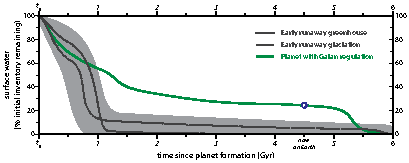
\includegraphics[width=1.0\linewidth]{figures/WaterInventory.pdf}
	\caption[Water loss on initially `wet' rocky planets]{
		Schematic illustration of the water loss caused by impacts and hydrogen escape.
		Hydrogen escape may entirely desiccate a rocky planet within a few billion years \citep{Lovelock2005}. Desiccation is inevitable as the host star luminosity increases, a cold trap is lost and the stratosphere becomes moist \citep{Lenton2001,OMalley-James2015}.}
	\label{fig:inventory}
\end{figure}
%%%%%%%%%%%%%%%%%%%%%%%%%%%%%%%%%%%%%%%%%%%%%%%%%%%%%%

However, the answer to the question ``Why didn't Earth undergo runaway greenhouse like Venus or a runaway glaciation like Mars?'' may have as much, or more, to do with life on Earth than with Earth's distance from the Sun.
The biotic mechanisms of how this preservation has been achieved have been discussed in the context of the Gaia Hypothesis by \citet{Harding2010}.

The early devolatilization of Earth-like planets around M-stars due to an extended pre-main sequence period of high extreme UV flux (above the dissociation energy of water, $\sim$5 eV)  could apply to some extent to Earth-like planets around more massive stars \citep{Luger2015,Tian2015}.

The amount of water (and volatiles in general) deposited or devolatilized during the late accretion phase of rocky planet formation in the universe is highly variable \citep{Raymond2004,Raymond2009} and can produce desert worlds \citep{Abe2011}, ocean worlds \citep{Leger2004}, and probably everything in between. Abiotic volatile evolution will be rapid, stochastic and hostage to the timing, mass, volatile content, and impact parameters of the largest impactors and the runaway feedbacks they could induce.

We argue that abiotic habitable zones are available initially and fleetingly to wet planets within a wide range of orbital radii ($\sim$0.5 to $\sim$2 AU) because of the thermal instability of their surfaces. Wide-ranging unstable temperatures could provide transitory abiotic habitable zones during the first half billion years after formation (\citet{Nisbet2002}, Figure \ref{fig:GaianHZ} B and \ref{fig:GaianHZ} C).

There are two ways to influence the surface temperature of a planet (Figure \ref{fig:feedbacks}): change the albedo (grey loops)  or  change the greenhouse gas content of the atmosphere (blue loops) \citep{Kasting2012}.
The amount and the phases of the volatiles (H$_{2}$O, CO$_{2}$, CH$_{4}$) of rocky planetary atmospheres control both the albedo and greenhouse warming.
Albedo and greenhouse warming, in turn, control the amount and phases of the volatiles. Strong positive feedback cycles (left side of Figure \ref{fig:feedbacks})  may lead to both i) runaway greenhouse (temperatures too hot for
life) with runaway loss of atmosphere (hydrogen loss and thus water loss) or ii) runaway glaciation (lowering the temperature and/or water activity to levels not conducive to life).

%%%%%%%%%%%%
\subsection{Implausibility of early negative feedback cycles}
\label{sec:silicateweathering}
In his original estimate of the continuous habitable zones, \citet{Hart1979} considered runaway greenhouse and runaway glaciation feedback but did not account for the negative feedback of silicate weathering on his models. The resulting continuous habitable zone of 0.95-1.01 AU had such a narrow width that he wrote:
\begin{quotation}
	It appears, therefore, that there are probably fewer planets in our galaxy suitable for the evolution of advanced civilizations than has previously been thought.
\end{quotation}

Such a narrow CHZ could help solve the Fermi paradox \citep[\eg,][Solution 36, p.158]{Webb2002}. More recent work has taken into account a stabilizing negative feedback loop associated with the recycling of CO$_2$ by plate tectonics. \citet{Walker1981} proposed a greenhouse-gas-based negative feedback process employing the carbonate-silicate cycle through the mechanism of silicate weathering. Increasing surface temperatures increases the silicate weathering rate, freeing up more Ca$^{2+}$ and other cations that combine with CO$_2$ (via aqueous bicarbonate HCO$_{3}^{-}$) to produce insoluble carbonates. Thus, when the temperature rises, more atmospheric CO$_2$ is sequestered and temperature decreases (Walker 1985, and the blue negative feedback loop on the right side of Figure \ref{fig:feedbacks}).
This abiotic negative feedback is largely responsible for moving the outer edge of the CHZ from 1.01 AU, as estimated by \citet{Hart1979}, to the more modern, larger values of 1.5-1.7 AU \citep[\eg,][]{Kasting1993a,Kopparapu2013}.

%%%%%%%%%%%%%%%%%%%%%%%%%%%%%%%%%%%%%%%%%%%%%%%%%%%%%%%%%%
\begin{figure*}[!tbp]
	\centering
	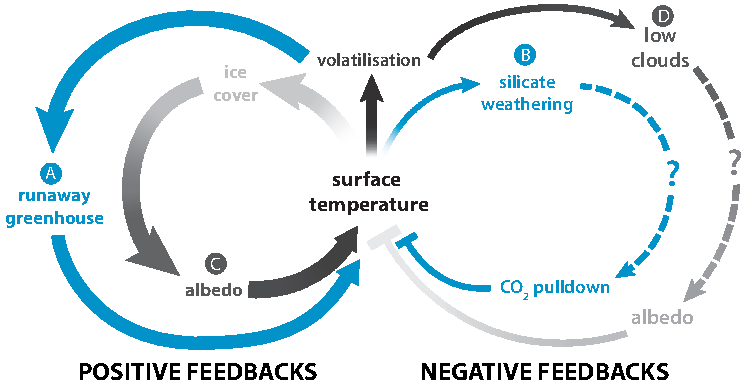
\includegraphics[width=0.9\linewidth]{figures/Feedback.pdf}
	\caption[Early abiotic feedbacks on Earth-like planets]{Early Abiotic Feedbacks.
		During the first billion years after the formation of Earth (or of Earth-like planets), abiotic positive feedbacks (left) can lead to runaway surface temperatures outside the habitable range (both too hot and too cold). These positive feedbacks lead to the loss of liquid water (either from hydrogen escape to space or condensation into ice (Figure \ref{fig:inventory})). Abiotic negative feedbacks (right) have been invoked to stabilize surface temperatures, but they may not be significant in the first billion years, hence the dashed lines
		and the question marks (Section \ref{sec:silicateweathering}).
		As life evolves, it can strengthen or weaken these initially abiotic geochemical feedback loops and turn them into biogeochemical cycles and feedback loops. Evolving life can insert itself into these feedbacks at the points labelled A, B, C and D. (Table \ref{tab:feedbacks} and Section \ref{sec:biofeedbacks}).
	}
	\label{fig:feedbacks}
\end{figure*}
%%%%%%%%%%%%%%%%%%%%%%%%%%%%%%%%%%%%%%%%%%%%%%%

%%%%%%%%%%%%%%%%%%%%%%%%%%%%%%%%%%%%%%%%%%%%%%%%%%%%%%%%%%
\begin{table*}[!ht]
	\centering
	\caption{Abiotic feedback processes active during the first billion years of a wet rocky planet's history and potential biotic enhancements of the feedback cycle.}
	\label{tab:feedbacks}
	\resizebox{1\textwidth}{!}{ 
		\begin{tabular}{l p{6.3cm} l p{7.2cm} }
			%{@{}lll|@{}}
			%\toprule
			Feedback       	& Mechanism	& Feedback Type		& Potential Biological Mediation\\
			\midrule
			greenhouse     	& greenhouse gases \citep{Ingersoll1969,Abe2011} 	 	& positive			& \textbf{A} \citep{Catling2001,Kasting2012,Goldblatt2009,Harding2010}\\
			greenhouse     	& silicate weathering \citep{Walker1981}   & negative?        	& \textbf{B} \citep{Lovelock1982,Schwartzman1989,Catling2001,Rosing2006,Honing2014}\\
			albedo          & ice albedo \citep{Budyko1969,Hoffman1998,Kopp2005}         & positive         	& \textbf{C} \citep{Harding2010,Watson1983}\\
			albedo          & low clouds \citep{Abe2011}          & negative?       	& \textbf{D} \citep{Rosing2010}\\  
			\bottomrule
		\end{tabular}
	}
	
\end{table*}
%%%%%%%%%%%%%%%%%%%%%%%%%%%%%%%%%%%%%%%%%%%%%%%%%%%%%%%%%


Since the temperature-dependent carbonate-silicate cycle provides a negative feedback, it could have been responsible for the long term stabilization of Earth's surface temperature. With a sufficiently high silicate weathering rate, even a lifeless planet could remain habitable. However, since temperature-dependent silicate weathering requires sub-aerial weathering of silicate rocks (either granitic or basaltic), the magnitude of the negative feedback of silicate weathering is roughly proportional to the amount of sub-aerial continental crust. In the first billion years of Earth's history, the fraction of the surface of Earth where sub-aerial erosion would have been possible may have been extremely small \citep{Flament2008,Abbot2012,Dhuime2015}. \citet{Flament2008} modeled the sub-aerial weathering as a function of time and estimated that in the late-Archean ($\sim$2.5 Gya)  2-3\%  of the Earth's surface was sub-aerial continent. The little continental crust present was largely submerged. Thus, it is likely that early in Earth's history, the negative feedback of the carbonate-silicate cycle may have been inoperative or at least significantly less effective than today. This undermines the main negative feedback mechanism proposed to stabilize surface temperature on wet rocky planets for the first billion years or so, when they are most likely to experience runaway greenhouse or runaway glaciation due to high inventories of primordial greenhouse gases, higher bombardment rates, and higher volcanism: hence, the ``?'' associated with this negative feedback loop in Figure \ref{fig:feedbacks} and Table \ref{tab:feedbacks}. Without this abiotic feedback cycle to extend the outer edge of the CHZ, the much narrower Hart-like continuously habitable zone (Figure \ref{fig:GaianHZ} B) becomes more plausible.

%%%%%%%%%%%%%%%%%%%%%%%%%%%%%%%%%%%%%%%%%%
\begin{figure*}[!htbp]
	\centering
	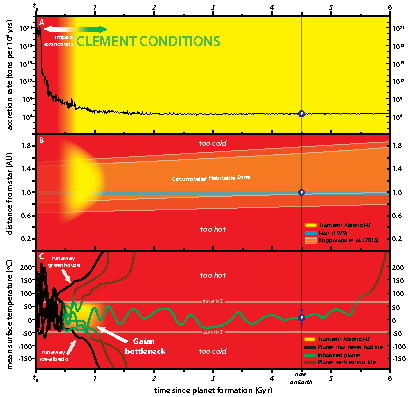
\includegraphics[width=0.9\linewidth]{figures/HZs.pdf}
	\caption[Habitable zones and the Gaian bottleneck]{
Bombardment, habitable zones, and the Gaian bottleneck.
\textbf{A}. Early heavy bombardment precludes life for the first $\sim$0.5 billion years, indicated by red in all three panels.
These impacts produce heat pulses and both deliver and remove volatiles \citep{Elkins-Tanton2011a}. 
Thus, the \textit{amount} of H$_{2}$O at the surface is highly variable during this period.
The \textit{phase} of the H$_{2}$O at the surface is also highly variable during this period because of impact-induced
alternation between greenhouse warming and ice-albedo runaway.
%
\textbf{B}. The width of the circumstellar habitable zone (CHZ) is usually considered to be a function of physics and chemistry, but
is often computed without the largely uncertain influence of clouds, and placed between Venus (0.7 AU) and Mars (1.5 AU). Here the blue region is from the work of \citet{Hart1979}, and the orange regions are based on estimates by \citet{Kopparapu2013} for the conservative (light orange) and optimistic (dark orange) limits. Life plays no role in these computations. The $\sim$30\% increase in the luminosity of the Sun since its formation is responsible for the outward migration of the traditional CHZ and some of the narrowness of Hart's continuously habitable zone.
The yellow zone in B represents our speculative version of a short-lived abiotic habitable zone at the tail end of the impact-induced
thermal instabilities shown in the first billion years of panel \textbf{C}.
The width of the abiotic habitable zone begins with a fairly wide range of semi-major axes, but lasts only from $\sim$0.5 to $\sim$1 Gyr
and then shrinks to zero.
After $\sim$1 Gyr, rapid impact-induced thermal excursions diminish and surface temperatures drift away and runaway from habitability.
Planets become devolatized because of the runaway greenhouse effect (top of panel C), 
and because liquid water condenses out into ice due to the runaway ice-albedo effect (bottom of panel C), with no abiotically stable zone between them.
The early evolution of Gaian regulation may be the main feature responsible for maintaining the surface temperature of Earth within a habitable range for the past $\sim$4 billion years \citep{Lovelock2000}.
	}
	\label{fig:GaianHZ}
\end{figure*}
%%%%%%%%%%%%%%%%%%%%%%%%%%%%%%%%%%%%%%%%%%%%%%%%%%%%%% 

The other abiotic negative feedback on surface temperature shown in Figure \ref{fig:feedbacks} is associated with low clouds:
higher temperatures  $\rightarrow$ more volatilization $\rightarrow$ more low altitude clouds  $\rightarrow$ higher albedo  $\rightarrow$ lower temperatures. Low clouds increase albedo and decrease surface temperatures more than they contribute towards raising the surface temperature because of the greenhouse effect associated with clouds \citep{Abe2011}. This is problematic because increasing volatilization produces both i) more low altitude clouds (which could cool Earth due to their higher albedo), and more high altitude clouds, which could have a stronger greenhouse effect than albedo effect and thus increase surfaces temperatures \citep{Goldblatt2011,Leconte2013}. For this reason, the effects of clouds are often considered the biggest source of uncertainty in global climate models and thus the ``?'' associated with this cycle in Figure \ref{fig:feedbacks} and Table \ref{tab:feedbacks}.

While it may be possible to vary albedo and greenhouse gases within some plausible range and construct a wide CHZ, without negative feedback, there is no justification for tuning these abiotic variables to maintain habitability. We postulate that the abiotic stabilizing feedbacks (two cycles on the right side of Figure \ref{fig:feedbacks}) were probably negligible
on early Earth. In their absence, it is hard to understand how habitability would have been maintained. Driver-less cars don't stay on roads. Without significant abiotic stabilization, we propose that the most plausible default becomes the abiotic tendency to evolve away from habitability shown in Figure \ref{fig:AHZ}
and Figure \ref{fig:GaianHZ} C.

Just because Earth is at 1 AU and has been inhabited for $\sim$4  billion years does not mean that there is a physics-based, biology-independent, computable continuous habitable zone. With thermal instability and increasing stellar luminosity, it is not clear that a physics-based continuously habitable zone even exists. There may be no range of orbital distances (or any region of multi-dimensional abiotic parameter space) for which the surface environments of initially wet rocky planets have sufficiently strong abiotic negative feedback to maintain habitability. If this is the case, purely abiotic computations of a continuously habitable zone may be misleading, and Gaian regulation becomes a plausible explanation for the continuously inhabited HZ in which we find ourselves.

%%%%%%%%%%%%%%%%%%%%%%%%%%%%%%%%

\section{The need for Gaia}
\label{sec:biofeedbacks}

It is usually assumed that the CHZ is determined by abiotic physical parameters: stellar mass and luminosity, planetary mass and 
atmospheric greenhouse gas composition, surface albedo, and sometimes clouds. 
More recently planetary spin, orbital eccentricity, obliquity, and initial water content have been added to the list of physical parameters \citep[\eg,][]{Gonzalez2005,Gaidos2005,Lammer2009,Gudel2014b,Shields2015}. %Armstrong et al 2014 
Here, we argue that these abiotic parameters can fleetingly enable the emergence of life but cannot maintain habitable surface conditions with liquid water.
As the early heavy bombardment subsides, strong selection pressure on life begins to regulate, control, and even dominate the mechanisms that 
create or maintain the temperatures and pressures at the surface of a planet that allow liquid water. If so, then biology (rather than physics or chemistry) can play the most important role in maintaining habitability.

In addition to the abiotic environmental changes (due to bombardment and devolatilization), there could be a long struggle that starts early between life and an environment that does not, abiotically, stay habitable. Feedback between life and environment may play the dominant role in maintaining the habitability of the few rocky planets in which life has been able to evolve Gaian regulation quickly.

If life gets started on a planet, there are many potential ways in which life can regulate the mechanisms that create or maintain 
the temperatures and pressures needed for liquid water \citep{Schneider1991,Schneider2004,Harding2010}. Gaia researchers propose that life on Earth evolved to become integrated into previously abiotic feedback systems that can modify or regulate surface temperature and the hydrological cycle \citep[\eg,][]{Lenton1998,Nisbet2012}. Life can evolve to enhance and regulate the feedback loops  (biological mediation processes A-D in Figure \ref{fig:feedbacks} and Table \ref{tab:feedbacks}).
Biologically mediated feedback loops are stabilizing or Gaian \citep{Ricklefs2000}. For habitability to be maintained, life could down-regulate the positive runaway feedback loops and enhance the negative feedback loops. On Earth, life began to modulate the greenhouse gases composition of the atmosphere as soon as life became widespread \citep{Nisbet2002,Nisbet2012,Nisbet2014,Johnson2015}.

The use of the Gaia hypothesis in ecology was reviewed by \citet{Free2007}. They argued (in agreement with \citet{Dawkins1982}) that selection for global stability is implausible.
However, they defined a Probable Homeostatic Gaia model: a planet ``with appropriate starting conditions for life will probably generate a biosphere the lifespan of which will be extended, rather than reduced, by life-environment feedback.'' In their Probable Homeostatic Gaia model, a ``network of life-environment interactions, largely dependent on the by-product effects of evolved traits, leads to global stability.''
This biology-based global stability is what we call Gaian regulation.  We are invoking its rapid evolution to stabilize the early volatile and thermal
instabilities of wet rocky planets.
%See Schneider \& Boston 1991 and Schneider et al 2004 for more discussion.
% cite O'Malley James and Cocknell 2015?

If Gaian regulation plays the dominant role in maintaining liquid water at the surface \citep{Harding2010}, then the width of the CHZ would depend more on 
the quirks of biological evolution than on the more deterministic physics and chemistry that can be more easily modeled. For most rocky planets in the CHZ to remain habitable, they may have to be inhabited:
``habitability depends on inhabitance and the width of the habitable zone is difficult to characterize'' \citep{Goldblatt2015}.


In Gaian literature, it is usually proposed that  Earth became a Gaian planet in the Proterozoic ($\sim$2.5 Gya) and has been one ever since \citep[p.45]{Harding2010}. We are proposing that the onset of Gaian regulation could have occurred more than a billion years earlier, for example, through the production, consumption, and regulation of greenhouse active gases such as H$_{2}$, CO$_{2}$, and CH$_{4}$. If there is a biotic solution for the faint early Sun paradox \citep{Sagan1972,Sagan1997,Feulner2012} based on higher concentrations of CO$_2$, on biotic methanogenesis, or on biotic albedo regulation, then this solution would necessarily have evolved quickly during the transient abiotic HZ (yellow regions in Figure \ref{fig:GaianHZ} B and C) \citep{Walker1985,Pavlov2003,Haqq-Misra2008,Rosing2010}.

\section{Evaluating the Gaian Bottleneck Hypothesis}

%%%%%%%%%%%%%%%%%%%%%%%%%%%%%%%%%%%%%%%%%%%%%%%%%%%%%%%%%%
\begin{figure*}[!b]
	\centering
	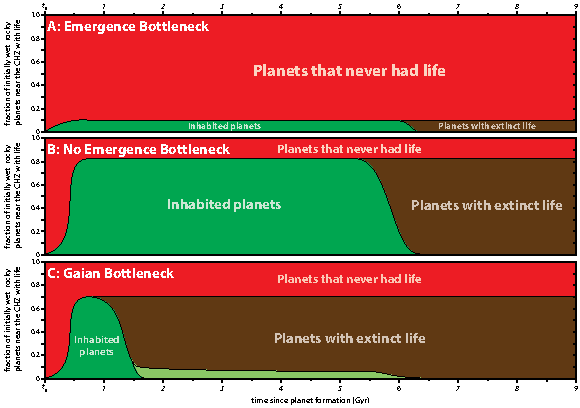
\includegraphics[width=0.9\linewidth]{figures/Summary.pdf}
	\caption[Different bottleneck scenarios]{Different bottleneck scenarios and their fossil predictions.
		\textbf{A}. Emergence Bottleneck: Life rarely emerges even on wet rocky planets. Few planets will have life or even fossils of extinct life.
		On the few planets where life does emerge, it persists for billions of years. 
		\textbf{B}. No Emergence Bottleneck.  Life emerges with high probability and usually persists for billions of years. Thus, life will be abundant on planets throughout the universe. There will be many planets where life persisted for billions of years and then went extinct. On the oldest uninhabited planets, fossils of complex  life will be abundant.
		\textbf{C}. Gaian Bottleneck. Life emerges with some probability (possibly quite high), but it goes extinct within a billion years (green). Alternatively, some small fraction of inhabited planets successfully pass through the Gaian bottleneck (light green). The Gaian bottleneck model predicts that the vast majority of the fossils in the universe will be from extinct microbial life.}
	\label{fig:summary}
\end{figure*}
%%%%%%%%%%%%%%%%%%%%%%%%%%%%%%%%%%%%%%%%%%%%%%%

After the early heavy bombardment, life emerges with some probability on initially wet rocky planets in the CHZ.
However, due to large impacts and unstable abiotic volatile evolution with no
tendency to maintain habitability, almost all life goes extinct early -- with the rare exceptions of life
that has undergone unusually rapid evolution and obtained some level of Gaian regulation. The most significant predictions of this Gaian bottleneck model can be seen in Figure \ref{fig:summary} by comparing panels A and B, with C.
In panels A and B, wherever life emerges, it persists for billions of years. Thus, it has time to evolve complex and perhaps multicellular forms. In panel C, which illustrates the Gaian bottleneck model, almost all emerging life goes extinct rapidly and therefore, does not have time to evolve into more complex forms.
However, even planets with Gaian regulation will not be able to counter indefinitely the increasing luminosity due to stellar evolution  \citep{Caldeira1992,Franck2000,Lenton2001,Franck2002,vonBloh2005}. Hence, the extinction at $\sim$6 Gyr in all 3 panels.

If we are able to find well-preserved, $\sim$3.8 to $\sim$4.3 billion year old rocks on Venus or Mars, then we may be able to identify
isotopic anomalies produced by biotic actions, in a way analogous to how $^{12}$C/$^{13}$C ratios are used to infer the existence of the earliest life in Isua, Greenland \citep{Ohtomo2014}. Whether it evolved independently of life on Earth will be difficult to determine. If we find evidence of extant life on Mars or Venus that had an origin independent of Earth life, then this would be evidence against both the Gaian bottleneck hypothesis and the emergence bottleneck.

The surface temperature and existence of liquid water at, or near, the surface could be predominantly due to Gaian regulation rather than abiotic negative  feedback. Liquid water on the surface of the planet (particularly old planets) would then not just be a prerequisite for life but a biosignature \citep{Gorshkov2004}. Existence of liquid water on the surface of a planet may be a better biosignature than oxygen \citep{Luger2015}. Thus, the measurement of exoplanet surface temperatures compatible with liquid water could be an important part of future search for extra-terrestrial life. Remote detection of atmospheric chemical equilibrium may soon develop into a mature science of remote bio-detection \citep[\eg,][]{Lovelock1975,Krissansen-Totton2016}. The Gaian bottleneck model predicts that the vast majority of the atmospheres of old terrestrial planets in the traditional abiotic CHZ of their host stars will be in chemical equilibrium because they are uninhabited. Hence, atmospheres in chemical disequilibrium will be rare except for young (t $\lesssim$ 2 Gyr) terrestrial planets.

In a critique of Gaian logic, \citet[p.236]{Dawkins1982} wrote:
\begin{quotation}
	For the analogy [of the Earth as an organism] to apply strictly, there would have to have been a set of rival Gaias, presumably on different planets. Biospheres which did not develop
	efficient homeostatic regulation of their planetary atmospheres tended to go extinct. The
	Universe would have to be full of dead planets whose homeostatic regulation systems had failed,
	with, dotted around, a handful of successful, well-regulated planets of which the Earth is one''.
\end{quotation}

What Dawkins describes here is also a prediction of the Gaian bottleneck hypothesis. The Gaian bottleneck model parallels evolution on Earth in that the vast majority ($\sim$99.9\%) of species that have ever lived are now extinct; the vast majority of planetary life has gone extinct.

In the far future, we may be able to find evidence for biogenic isotopic anomalies on the initially wet rocky planets around most stars. Since life does not persist for long in the Gaian bottleneck model, it predicts a universe filled with isotopic or microscopic fossils
from the kind of life that can evolve in $\sim$1 Gyr, not the fossils of larger multicellular eukaryotes or anything else that would take several billion years to evolve.

\citet{Cockell2014} divided all environments in the Universe into three types: (1) uninhabitable, (2) uninhabited habitats or (3) inhabited habitats \citep{Cockell2011,Zuluaga2014}. A prediction of the Gaian bottleneck (persistence-is-hard) model is that (2) and (3) will be rare. This is unfortunate for future colonization efforts since uninhabited, but habitable, planets are the most ethically appealing places -- autochthonous life would not have to be displaced.

Our search for life beyond Earth may be thwarted by the short time-scales over which planets may remain inhabited. If it takes several billion years to develop radio telescopes, then the Gaian bottleneck ensures that the vast majority of life in the universe is either young and microbial, or extinct. Therefore, the Gaian bottleneck model is consistent with current SETI results and can help resolve the Fermi paradox, although it is not one of the solutions to the paradox listed by \citet{Webb2002}.
%%%%%%%%%%%%%%%%%%%%%%%%%%%%%%%%%%%%%%%%

	
\clearpage
\section{What could be wrong with our argument?}
\begin{enumerate}
	\item Gaian regulation is a controversial idea.  It is usually invoked to explain the long-term stability of the surface temperature of Earth, starting in the Proterozoic ($\sim$2.5 Gya). So invoking early, pre-Proterozoic Gaia is even more controversial.
	
	\item If estimates of sub-aerial continental crust \citep[\eg, by][]{Flament2008} are significantly too low and there was abundant sub-aerial crust earlier than  
	$\sim$3.8 Gya \citep[\eg,][]{VanKranendonk2010}, then abiotic negative feedback based on the
	carbonate-silicate cycle could have stabilized surface temperatures very early in Earth's history, without Gaian regulation. If early continent formation
	is a common feature of rocky planets, then invoking Gaian regulation may be unnecessary to explain Earth's early thermal stability.
	
	\item We are arguing that:
	\begin{enumerate}
		\item Gaian regulation evolved on Earth.
		\item The evolution of Gaian regulation is not common.
	\end{enumerate}
	This could seem paradoxical, because to justify (a), we have presented arguments making the emergence of Gaian regulation plausible. 
	These same arguments could suggest that Gaian regulation would be common. However, there is a large class of phenomena that did happen on Earth, that are uncommon or non-existent elsewhere.
	We can trace the evolution of these phenomena and explain how they evolved on Earth, but these explanations cannot be generalized.
	For example, the evolution of the English language can be traced and understood and made plausible, but this plausibility cannot be turned 
	into a generic argument for the evolution of English on other planets. 
	Human-like intelligence may be another member of this class \citep{Lineweaver2008}. We are suggesting that the evolution of a kind of life that can quickly and effectively regulate the volatiles on the surface of the planet on which it finds itself, may be a quirky product of the biological evolution of life on early Earth.
	
	\item Why should Gaian regulation be rare? \citet{Franck2002,Franck2001} concluded that there are $\sim$500,000 ``sister Gaias'' in the Milky Way galaxy but then listed a number of physical factors \citep[\eg, those discussed by][]{Ward2000} that could reduce this estimate.
	
	\item It could be that early heavy impacts almost always extinguish life and don't need any help from subsequent volatile evolution away from habitability. In which case, Gaian regulation would have nothing to do with life's early or late extinction. Evidence for this would be an anomalously low impact rate on Earth (compared to the early impact rates on other wet rocky planets). If this were the case, there would be no tendency for life to evolve and regulate its environment. In this context, \citet{Tyrrell2013} suggested that ``Lucky Gaia'' as described by \citet{Free2007}, and the anthropic principle provide a better explanation for the continued habitability of Earth than ``Probable Gaia,'' which we assume here.
	
	If the probability of the emergence and persistence of life on wet rocky planets were infinitesimally small and there were only one life-harboring planet in the Universe, we would, of necessity, find ourselves on that planet. Therefore, our mere existence cannot be used to infer the probability of life elsewhere. Additionally, invoking a scenario in which persistent life on Earth is exceptional compared to other planets (as we do here) cannot be criticized with an argument such as: if Gaian regulation is rare, then we shouldn't be here. Self-selection overcomes this critique. 

	\item One argument against early Gaian regulation is that the unit of biological selection starts small and moves to larger groups as in the chronological sequence: genes, chromosomes, single cells, colonies of cells (bacterial mats), multicellular organisms, colonies of multicellular organisms (superorganisms), ecosystems of various sizes (which produce Gaian regulation only when they are widespread). In this sequence, the evolution of Gaian regulation happens last. However, among the earliest life forms we know of, stromatolites were already ecosystems of bacterial mats \citep{Walter1992}.
	
	\item The universe does not seem to be teeming with life.
	This could be an observational selection effect: it is teeming with life but we just haven't been able to detect it yet. Even in the future when the remote detection of biosignatures is possible, it will be difficult to detect subsurface life \citep{Boston1992,Gaidos1999,Jones2011,McMahon2013} that does not interact with the planet's atmosphere and is completely sustained by free energy based on geochemical disequilibrium.
	This would undermine some of the motivation for the Gaian bottleneck model but not the other arguments presented here.
\end{enumerate}


\section{Conclusion}
We are proposing a potentially universal sequence of events on initially wet rocky planets that can be summarized thusly:
\begin{itemize}
	\item[]\textbf{First $\sim$0.5 Gyr:} Hot, high bombardment, uninhabitable.
	\item[]\textbf{$\sim$0.5 to $\sim$1.0 Gyr:} Cooler, reduced bombardment, continuous volatile loss.
	\item[]\textbf{$\sim$0.5 to $\sim$1.0 Gyr:} Emergence of life in an environment with a tendency to evolve away from habitability
	\item[]\textbf{$\sim$1.0 to $\sim$1.5 Gyr:} Inability to maintain habitability, followed by extinction.
	As a rare alternative, this period would experience the rapid evolution of Gaian regulation and the maintenance of habitability, followed by the persistence of life for several billion more years. 
\end{itemize}
Between the early heat pulses, freezing, volatile content variation, and runaway positive feedbacks, maintaining life on an initially wet rocky planet in the habitable zone may be like trying to ride a wild bull. Most life falls off.  Life may be rare in the universe, not because it is difficult to get started, but because habitable environments are difficult to maintain during the first billion years.

In the book \textit{Vital Dust}, \citet{DeDuve1995} presented the case that water and energy are common and abiogenesis may be a cosmic imperative. The most important constraint on the existence of life in the universe may be whether life, after emerging and evolving into a biosphere, can evolve global mechanisms 
rapidly enough to mediate the positive and negative feedbacks of abiotic atmospheric evolution. We hypothesize that the early evolution of biologically mediated negative feedback processes, or Gaian regulation as proposed by \citet{Lovelock1974}, may be necessary to maintain habitability because of the strength, rapidity, and universality of abiotic positive feedbacks on the surfaces of rocky planets in traditional CHZs.

We argue that the habitable surface environments of rocky planets usually become uninhabitable due to abiotic runaway positive feedback mechanisms involving surface temperature, albedo, and the loss of atmospheric volatiles. Because of the strength, rapidity, and universality of abiotic positive feedbacks in the atmospheres of rocky planets in traditional CHZs, biotic negative feedback or Gaian regulation may be necessary to maintain habitability.

The evolution of biospheric regulation of surface volatiles, temperature, and albedo can become a Gaian bottleneck to the persistence of life. This Gaian bottleneck may be a better explanation for the non-prevalence of life than the traditional emergence bottleneck paradigm. 


%----------------------------------------------------------------------------------------
%	BIBLIOGRAPHY
%----------------------------------------------------------------------------------------
%Use the executable file provide here to clean-up Mendeley generated bib files
%https://ramblingacademic.com/2016/06/19/fixing-bibtex-files-mendeley/ 
% or the python script at https://tex.stackexchange.com/questions/286261/incompatible-month-formats-between-biblatex-and-mendeley

\printbibliography[heading=bibintoc]

%----------------------------------------------------------------------------------------
%----------------------------------------------------------------------------------------
%	THESIS CONTENT - APPENDICES
%----------------------------------------------------------------------------------------

\appendix % Cue to tell LaTeX that the following "chapters" are Appendices

% Include the appendices of the thesis as separate files from the Appendices folder
% Uncomment the lines as you write the Appendices

% Appendix A

\chapter{Codes} % Main appendix title

\label{AppendixA} % For referencing this appendix elsewhere, use \ref{AppendixA}

\section{Python models}

\renewcommand\listingscaption{Model}
\renewcommand\listoflistingscaption{List of ArcGIS Models}

\newmintedfile[pythoncode]{python}{
bgcolor=mintedbackground,
fontfamily=tt,
linenos=true,
numberblanklines=false,
numbersep=5pt,
gobble=0,
frame=lines,
framerule=0.3pt,
framesep=2mm,
funcnamehighlighting=true,
tabsize=4,
obeytabs=false,
mathescape=false,
samepage=true, %with this setting you can force the list to appear on the same page
showspaces=false,
showtabs=false,
texcl=false,
breaklines=true,
fontsize=\footnotesize,
baselinestretch=0.9,
firstline=5,
numbers=left,
firstnumber=1,
stepnumber=1,
breakanywhere=true
% breakautoindent=true,
% autogobble=true,
% python3=true,
}

Example to check whether an integer is a prime number or not using for loop and if...else statement.

A positive integer greater than 1 which has no other factors except 1 and the number itself is called a prime number. 2, 3, 5, 7 etc. are prime numbers as they do not have any other factors.
\begin{listing}[H]
\pythoncode{Code/Prime.py}
\caption{Python Program to Check Prime Number}\label{Code:Prime}
\end{listing}
%%!TEX root = ../main.tex

% Appendix B

\chapter{Proofs of key results in Chapter \ref{ch:evaluating_decisions}} % Main appendix title

\label{AppendixB} % For referencing this appendix elsewhere, use \ref{AppendixA}

\section{IO Contractibility}\label{sec:io_contract_proof}

\subsection{Equality of equally sized contractions}

This is the proof of Theorem \ref{th:equal_of_condits}.

All swaps can be written as a product of transpositions, so proving that a property holds for all finite transpositions is enough to show it holds for all finite swaps. It's useful to define a notation for transpositions.

\begin{definition}[Finite transposition]
Given two equally sized sequences $A,B\in \mathbb{N}^n$ with $A=(a_i)_{i\in [n]}$, $B=(b_i)_{i\in [n]}$, ${A\rightarrow B}:\mathbb{N}\to \mathbb{N}$ is the permutation such that 
\begin{align}
	[A\rightarrow B](a_i) = b_i
\end{align}that sends the $i$th element of $A$ to the $i$th element of $B$ and vise versa. Note that $B\rightarrow A$ is the inverse of $A\rightarrow B$.
\end{definition}

Lemma \ref{lem:infinitely_extended_kernels} is used to extend conditional probabilities of finite sequences to infinite ones. 

\begin{lemma}[Infinitely extended kernels]\label{lem:infinitely_extended_kernels}
Given a collection of Markov kernels $\kernel{K}_i:W\times X^{\mathbb{N}}\kto Y^i$ for all $i\in \mathbb{N}$, if we have for every $j>i$
\begin{align}
    \kernel{K}_j(\text{id}_{Y^i}\otimes \text{Del}_{Y^{j-i}}) &= \kernel{K}_i\otimes \text{Del}_{X^{j-i}}\label{eq:marginalise_comb}
\end{align} 
then there is a unique Markov kernel $\kernel{K}:X^{\mathbb{N}}\kto Y^{\mathbb{N}}$ such that for all $i,j\in \mathbb{N}$,$j>i$
\begin{align}
    \kernel{K}(\text{id}_{Y^i}\otimes \text{Del}_{Y^{\mathbb{N}}})&= \kernel{K}_i\otimes \text{Del}_{X^{j-i}}
\end{align}
\end{lemma}

\begin{proof}
Take any $x\in X^{\mathbb{N}}$ and let $x_{|m}\in X^n$ be the first $n$ elements of $x$. By Equation \eqref{eq:marginalise_comb}, for any $A_i\in \sigalg{Y}$, $i\in [m]$
\begin{align}
    \kernel{K}_n(\bigtimes_{i\in [m]}A_i\times Y^{n-m}|x_{|n}) &= \kernel{K}_m(\bigtimes_{i\in [m]}A_i|x_{|m})
\end{align}

Furthermore, by the definition of the $\mathrm{Swap}$ map for any permutation $\rho:[n]\to[n]$
\begin{align}
    \kernel{K}_n\mathrm{Swap}_{\rho}(\bigtimes_{i\in [m]}A_{\rho(i)}\times Y^{n-m}|x_{|n}) &= \kernel{K}_n(\bigtimes_{i\in [m]}A_{i}\times Y^{n-m}|x_{|n})
\end{align}
thus by the Kolmogorov Extension Theorem \citep{cinlar_probability_2011}, for each $x\in X^{\mathbb{N}}$ there is a unique probability measure $\prob{Q}_x\in \Delta(Y^{\mathbb{N}}$ satisfying
\begin{align}
    \prob{Q}_x(\bigtimes_{i\in [n]}A_i\times Y^{\mathbb{N}}) &= \kernel{K}_n(\bigtimes_{i\in [n]}A_{\rho(i)}|x_{[n]})\label{eq:q_is_Markov}
\end{align}

Furthermore, for each $\{A_i\in\sigalg{Y}|i\in \mathbb{N}\}$, $n\in \mathbb{N}$ note that for $p>n$
\begin{align}
\prob{Q}_x(\bigtimes_{i\in[n]} A_i \times Y^{\mathbb{N}})&\geq \prob{Q}_x(\bigtimes_{i\in [p]} A_i\times Y^{\mathbb{N}})\\
&\geq \prob{Q}_x(\bigtimes_{i\in \mathbb{N}} A_i)
\end{align}
so by the Monotone convergence theorem, the sequence $\prob{Q}_x(\bigtimes_{i\in[n]} A_i)$ converges as $n\to \infty$ to $\prob{Q}_x(\bigtimes_{i\in\mathbb{N}} A_i)$. $x\mapsto \prob{Q}_x^{\RV{Z}_n}(\bigtimes_{i\in[n]} A_i)$ is measurable for all $n$, $\{A_i\in\sigalg{Y}|i\in \mathbb{N}\}$ by Equation \eqref{eq:q_is_Markov}, and so $x\mapsto Q_x$ is also measurable.

Thus $x\mapsto Q_x$ is the desired Markov kernel $\kernel{K}$.
\end{proof}

\begin{corollary}\label{cor:equal_subconditionals}
Given $(\prob{P}_C,\Omega,\sigalg{F})$, $\RV{W}:\Omega\to V$ and two pairs of sequences $(\RV{V},\RV{X}):=(\RV{V}_i,\RV{X}_i)_{i\in\mathbb{N}}$ and $(\RV{Y},\RV{Z}):=(\RV{Y}_i,\RV{Z}_i)_{i\in \mathbb{N}}$ with corresponding variables taking values in the same sets $V=Y$ and $X=Z$, if $(\prob{P}_C,\RV{V},\RV{X})$ and $(\prob{P}_C,\RV{Y},\RV{Z})$ are both local over $\RV{W}$ and
\begin{align}
    \prob{P}^{\RV{X}_{[n]}|\RV{W}\RV{V}_{[n]}} &= \prob{P}^{\RV{Z}_{[n]}|\RV{W}\RV{Y}_{[n]}}
\end{align}
for all $n\in\mathbb{N}$ then
\begin{align}
    \prob{P}^{\RV{X}|\RV{W}\RV{V}} &= \prob{P}^{\RV{Z}|\RV{W}\RV{Y}}
\end{align}
\end{corollary}

\begin{proof}
By assumption of locality
\begin{align}
    \prob{P}^{\RV{X}_{[n]}|\RV{W}\RV{V}_{[n]}}\otimes\mathrm{Del}_{W^\mathbb{N}} &= \prob{P}^{\RV{X}|\RV{W}\RV{V}}(\mathrm{id}_{X^n}\otimes \mathrm{Del}_{X^{\mathbb{N}}})\\
    \prob{P}^{\RV{Z}_{[n]}|\RV{W}\RV{Y}_{[n]}}\otimes\mathrm{Del}_{W^\mathbb{N}} &= \prob{P}^{\RV{Z}|\RV{W}\RV{Y}}(\mathrm{id}_{X^n}\otimes \mathrm{Del}_{X^{\mathbb{N}}})
\end{align}
hence for all $n,m>n$
\begin{align}
    \prob{P}^{\RV{X}_{[m]}|\RV{W}\RV{V}_{[m]}}(\mathrm{id}_{X^n}\otimes \mathrm{Del}_{X^{m-n}}) &= \prob{P}^{\RV{Z}_{[m]}|\RV{V}\RV{Y}_{[m]}}(\mathrm{id}_{X^n}\otimes \mathrm{Del}_{X^{m-n}})\\
    &= \prob{P}^{\RV{X}_{[n]}|\RV{W}\RV{V}_{[n]}}\otimes\mathrm{Del}_{W^{m-n}}
\end{align}
and, in particular, by lemma \ref{lem:infinitely_extended_kernels}, $\prob{P}^{\RV{X}|\RV{W}\RV{V}}$ and $\prob{P}^{\RV{Z}|\RV{W}\RV{Y}}$ are the limits of the same sequence.
\end{proof}

\begin{theorem}[Graphical representation of exchange commutativity]
A sequential input-output model $(\prob{P}_C,\RV{D},\RV{Y})$ along with some $\RV{W}:\Omega\to W$ commutes with exchange over $\RV{W}$ if and only if for every $\alpha$, every finite permutation $\rho:\mathbb{N}\to\mathbb{N}$ and corresponding swap map $\mathrm{Swap}_\rho:X^{\mathbb{N}}\kto X^{\mathbb{N}}$
\begin{align}
    \tikzfig{exch_com_lhs} &= \tikzfig{exch_com_rhs}
\end{align}
\end{theorem}

\begin{proof}
This follows from the fact that
\begin{align}
    \prob{P}_\alpha^{\RV{Y}_\rho|\RV{W}\RV{D}_{\rho}} = \tikzfig{exch_com_rhs}
\end{align}
To see this, note that
\begin{align}
    &\tikzfig{exch_com_rhs}(\bigtimes_{i\in \mathbb{N}} A_i|w,(d_i)_\mathbb{N})\\
     &= \prob{P}_\alpha^{\RV{Y}|\RV{W}\RV{D}}(\bigtimes_{i\in \mathbb{N}}A_{\rho^{-1}(i)}|w,(d_{\rho^{-1}(i)})_\mathbb{N})\\
    &= \prob{P}_\alpha^{\RV{Y}_\rho|\RV{W}\RV{D}_\rho}(\bigtimes_{i\in \mathbb{N}}A_i|w,(d_i)_\mathbb{N})
\end{align}
\end{proof}

The main proof follows.

\begin{reptheorem}{th:equal_of_condits}
Given a sequential input-output model $(\prob{P}_C,\RV{D},\RV{Y})$ and some $\RV{W}$, $\prob{P}_\alpha^{\RV{Y}|\RV{WD}}$ is IO contractible over $\RV{W}$ if and only if for all subsequences $A,B\subset \mathbb{N}^{|A|}$ and for every $\alpha$
\begin{align}
    \prob{P}_\alpha^{\RV{Y}_A|\RV{WD}_{A,\mathbb{N}\setminus A}} &= \prob{P}_\alpha^{\RV{Y}_B|\RV{WD}_{B,\mathbb{N}\setminus B}}\\
    &= \prob{P}_\alpha^{\RV{Y}_A|\RV{WD}_A}\otimes \text{del}_{D^{|\mathbb{N}\setminus A|}}
\end{align}
\end{reptheorem}

\begin{proof}
Only if:
For $Z\in \mathbb{N}^{|A|}$, let $\text{del}_{Z^\complement}$ be the Markov kernel associated with the map that sends $\RV{Y}$ to $\RV{Y}_Z:=(\RV{Y}_i)_{i\in Z}$.

If $A$ is finite, then let $n:=|A|$ and by exchange commutativity
\begin{align}
        \prob{P}_\alpha^{\RV{Y}_A|\RV{WD_{A,\mathbb{N}\setminus A}}}&= \prob{P}_\alpha^{\RV{Y}_A|\RV{WD_{A\rightarrow [n]}}}\\
         &= \prob{P}_\alpha^{\RV{Y}|\RV{WD_{A\rightarrow [n]}}}\text{del}_{A^{\complement}}\\
        &=  \prob{P}_\alpha^{\RV{Y}_{[n]\rightarrow A}|\RV{WD}}\text{del}_{A^{\complement}}
\end{align}
Use the fact that $[n]\rightarrow A \circ B\rightarrow [n]= B\rightarrow A$ and apply exchange commutativity to get
\begin{align}
	\prob{P}_\alpha^{\RV{Y}_{[n]\rightarrow A}|\RV{WD}}\kernel{F}_{\Pi_{A}} &= \prob{P}_\alpha^{\RV{Y}_{B\rightarrow A}|\RV{WD}_{B\rightarrow [n]}}\text{del}_{A^{\complement}}\\
	&= \prob{P}_\alpha^{\RV{Y}|\RV{WD}_{B\rightarrow [n]}}\text{del}_{B^{\complement}}\\
	&= \prob{P}_\alpha^{\RV{Y}_B|\RV{WD_{B,\mathbb{N}\setminus B}}}
\end{align}

if $A$ is infinite, then we can take finite subsequences $A_m$ that are the first $m$ elements of $A$ and similarly for $B_m$. Then by previous reasoning
\begin{align}
            \prob{P}_\alpha^{\RV{Y}_{A_m}|\RV{WD_{A_m\rightarrow [m]}}} &= \prob{P}_\alpha^{\RV{Y}_{[m]}|\RV{WD}}\\
        &= \prob{P}_\alpha^{\RV{Y}_{B_m}|\RV{WD_{B_m\rightarrow [m]}}}
\end{align}
then by Corollary \ref{cor:equal_subconditionals}
\begin{align}
\prob{P}_\alpha^{\RV{Y}_A|\RV{WD_{A\rightarrow [n]}}}=\prob{P}_\alpha^{\RV{Y}_{B_m}|\RV{WD_{B_m\rightarrow [m]}}}
\end{align}

Finally, by locality
\begin{align}
    \prob{P}_\alpha^{\RV{Y}_A|\RV{WD_{A\rightarrow [n]}}} &= \prob{P}_\alpha^{\RV{Y}_A|\RV{WD}_A}\otimes \text{Del}_{D^{|\mathbb{N}\setminus A}}
\end{align}

If:
Taking $A=[n]$ for all $n$ establishes locality, and taking $A=(\rho(i))_{i\in \mathbb{N}}$ for arbitrary finite permutation $\rho$ establishes exchange commutativity.
\end{proof}

\section{Tabulated conditional distributions}\label{sec:io_contract_models}

This is the proof of Lemmas \ref{th:table_rep_kernel} and \ref{lem:ciid_yd} and Theorem \ref{th:any_infinite_sequence}. The following definitions are reproduced for convenience.

\begin{repdefinition}{def:count_of_inputs}
Given a sequential input-output model $(\prob{P}_C,\RV{D},\RV{Y})$ on $(\Omega,\sigalg{F})$ with countable $D$, $\#_{j}^k$ is the variable
\begin{align}
    \#_{j}^k := \sum_{i=1}^{k-1} \llbracket \RV{D}_i = j \rrbracket
\end{align}
In particular, $\#_{j}^k$ is equal to the number of times $\RV{D}_i=j$ over all $i<k$.
\end{repdefinition}

\begin{repdefinition}{def:tab_cd}
Given a sequential input-output model $(\prob{P}_C,\RV{D},\RV{Y})$ on $(\Omega,\sigalg{F})$, define the tabulated conditional distribution $\RV{Y}^D:\Omega\to Y^{\mathbb{N}\times D}$ by
\begin{align}
    \RV{Y}^D_{ij} = \sum_{k=1}^{\infty} \llbracket \#_j^k = i-1\rrbracket \llbracket \RV{D}_k = j \rrbracket \RV{Y}_k
\end{align}
That is, the $(i,j)$-th coordinate of $\RV{Y}^D(\omega)$ is equal to the coordinate $\RV{Y}_k(\omega)$ for which the corresponding $\RV{D}_k(\omega)$ is the $i$th instance of the value $j$ in the sequence $(\RV{D}_1(\omega),\RV{D}_2(\omega),...)$, or 0 if there are fewer than $i$ instances of $j$ in this sequence.
\end{repdefinition}

The proof of the theorem follows.

\begin{replemma}{th:table_rep_kernel}
Suppose a sequential input-output model $(\prob{P}_C,\RV{D},\RV{Y})$ is given with $D$ countable and $\RV{D}$ infinitely supported. Then for some $\RV{W}$, $\alpha$, $\prob{P}_\alpha^{\RV{Y}|\RV{WD}}$ is IO contractible if and only if
\begin{align}
    \prob{P}_\alpha^{\RV{Y}|\RV{WD}} &= \tikzfig{lookup_representation_kernel}\label{eq:lup_rep_kernel}\\
    &\iff\\
    \prob{P}_\alpha^{\RV{Y}|\RV{WD}}(\bigtimes_{i\in \mathbb{N}}A_i|w,(d_i)_{i\in \mathbb{N}}) &= \prob{P}_\alpha^{(\RV{Y}^D_{i d_i})_{i\in\mathbb{N}}|\RV{W}}(\bigtimes_{i\in \mathbb{N}}A_i|w)&\forall A_i\in \sigalg{Y}^{D}, w\in W, d_i\in D
\end{align}
Where $\prob{F}_{\text{lu}}$ is the Markov kernel associated with the lookup map
\begin{align}
    \text{lu}:X^\mathbb{N}\times Y^{\mathbb{N}\times D}&\to Y\\
    ((x_i)_\mathbb{N},(y_{ij})_{i,j\in \mathbb{N}\times D})&\mapsto (y_{i d_i})_{i\in \mathbb{N}}
\end{align}
and for any finite permutation within rows $\eta:\mathbb{N}\times D\to \mathbb{N}\times D$
\begin{align}
    \prob{P}_\alpha^{(\RV{Y}^D_{ij})_{\mathbb{N}\times D}|\RV{W}}&= \prob{P}_\alpha^{(\RV{Y}^D_{\eta(i,j)})_{\mathbb{N}\times D}|\RV{W}}\label{eq:col_exch}
\end{align}
\end{replemma}

\begin{proof}
Only if:
We define a random invertible function $\RV{R}:\Omega\times \mathbb{N}\to \mathbb{N}\times {D}$ that reorders the indicies so that, for $i\in \mathbb{N},j\in D$, $\RV{D}_{\RV{R}^{-1}(i,j)}=j$ almost surely. We then use IO contractibility to show that $\prob{P}_\alpha^{\RV{Y}|\RV{D}}(\cdot|d)$ is equal to the distribution of the elements of $\RV{Y}^D$ selected according to $d\in D^{\mathbb{N}}$.

Note that at most one of $\llbracket \#_j^k = i-1\rrbracket\llbracket \RV{D}_k=j\rrbracket$ and $\llbracket \#_j^l = i-1\rrbracket\llbracket \RV{D}_l=j\rrbracket$ can be greater than 0 for $k\neq l$ and, by assumption, $\sum_{j\in D}\sum_{k\in \mathbb{N}} \llbracket \#_j^k = i-1\rrbracket\llbracket \RV{D}_k=j\rrbracket=1$ almost surely (that is, for any $i,j$ there is some $k$ such that $\RV{D}_k$ is the $i$th occurrence of $j$). Define $\RV{R}_k:\Omega\to \mathbb{N}\times D$ by $\omega \mapsto \argmax_{i\in\mathbb{N},j\in D} \llbracket \#_j^k = i-1\rrbracket\llbracket \RV{D}_k=j\rrbracket(\omega)$ (i.e. $\RV{R}_k$ returns the $(i,j)$ pair where $j$ is the value of $\RV{D}_k$ and $i$ is the count of $j$ occurrences up to $\RV{D}_k$). Let $\RV{R}:\mathbb{N}\to \mathbb{N}\times D$ by $k\mapsto \RV{R}_k$. $\RV{R}$ is almost surely bijective and 
\begin{align}
    \RV{Y}^D&:= (\RV{Y}^D_{ij})_{i\in \mathbb{N},j\in D}\\
    &= (\RV{Y}_{\RV{R}^{-1}(i,j)})_{i\in \mathbb{N},j\in D}\\
    &=: \RV{Y}_{\RV{R}^{-1}}
\end{align}

By construction, $\RV{D}_{\RV{R}^{-1}(i,j)}=j$ almost surely; that is, $\RV{D}_{\RV{R}^{-1}}$ is a single-valued variable. In particular, it is almost surely equal to $e:=(e_{ij})_{i\in\mathbb{N},j\in D}$ such that $e_{ij}=j$ for all $i$. Hence
\begin{align}
    \prob{P}_\alpha^{\RV{Y}^D|\RV{W}\RV{D}_{\RV{R}^{-1}}}(A|w,d)&= \prob{P}_\alpha^{\RV{Y}_{\RV{R}^{-1}}|\RV{W}\RV{D}_{\RV{R}^{-1}}}(A|w,d)\\
    &\overset{\prob{P}_C}{\cong} \prob{P}_\alpha^{\RV{Y}_{\RV{R}^{-1}}|\RV{W}\RV{D}_{\RV{R}^{-1}}}(A|w,e)\label{eq:yd_is_indep}\\
    &= \prob{P}_\alpha^{\RV{Y}^D}(A|w)\label{eq:yd_dist}
\end{align}
for any $d\in D^{\mathbb{N}}$.

Now,
\begin{align}
    \prob{P}^{\RV{Y}_{\RV{R}^{-1}}|\RV{W}\RV{D}_{\RV{R}^{-1}}}_\alpha(A|w,d) &= \int_R \prob{P}_\alpha^{\RV{Y}_\rho|\RV{W}\RV{D}_{\rho}}(A|d)\prob{P}_\alpha^{\RV{R}^{-1}|\RV{W}\RV{D}_{\RV{R}^{-1}}}(\mathrm{d}\rho|w,d)\label{eq:need_ccont}\\
\end{align}
For each $\rho$, define $\rho^n:\mathbb{N}\to \mathbb{N}$ as the finite permutation that agrees with $\rho$ on the first $n$ indices and is the identity otherwise. By IO contractibility, for $n\in \mathbb{N}$
\begin{align}
    \prob{P}^{\RV{Y}_{\rho^n([n])}|\RV{W}\RV{D}_{\rho^n([n])}} &= \prob{P}^{\RV{Y}_{\rho([n])}|\RV{W}\RV{D}_{\rho([n])}}\\
    &= \prob{P}^{\RV{Y}_{[n]}|\RV{W}\RV{D}_{[n]}}
\end{align}
By Corollary \ref{cor:equal_subconditionals}, it must therefore be the case that
\begin{align}
    \prob{P}^{\RV{Y}|\RV{W}\RV{D}} = \prob{P}^{\RV{Y}_{\rho}|\RV{W}\RV{D}_{\rho}}
\end{align}
Then from Equation \eqref{eq:need_ccont}
\begin{align}
    \prob{P}^{\RV{Y}_{\RV{R}^{-1}}|\RV{W}\RV{D}_{\RV{R}^{-1}}}_\alpha(A|w,d) &\overset{\prob{P}_C}{\cong} \int_R \prob{P}_\alpha^{\RV{Y}_\rho|\RV{W}\RV{D}_{\rho}}(A|d)\prob{P}_\alpha^{\RV{R}^{-1}|\RV{W}\RV{D}_{\RV{R}^{-1}}}(\mathrm{d}\rho|w,d)\\
    &\overset{\prob{P}_C}{\cong} \int_R \prob{P}_C^{\RV{Y}|\RV{WD}}(A|w,d)\prob{P}_\alpha^{\RV{R}^{-1}|\RV{W}\RV{D}_{\RV{R}^{-1}}}(\mathrm{d}\rho|w,d)\\
    &\overset{\prob{P}_C}{\cong} \prob{P}_C^{\RV{Y}|\RV{WD}}(A|w,d)\label{eq:rotated_conditional}
\end{align}
 for all $i,j\in \mathbb{N}$. Then by Equation \eqref{eq:yd_dist} and Equation \eqref{eq:rotated_conditional}
\begin{align}
    \prob{P}_\alpha^{\RV{Y}^D|\RV{W}}(A|w) &= \prob{P}_\alpha^{\RV{Y}|\RV{WD}}(A|w,e)\label{eq:rel_bet_y_yd}
\end{align}

Take some $d\in D^{\mathbb{N}}$. From Equation \eqref{eq:rel_bet_y_yd} and IO contractibility of $\prob{P}_C^{\RV{Y}|\RV{WD}}(A|e)$,
\begin{align}
    (\prob{P}_\alpha^{\RV{Y}^D|\RV{W}}\otimes \mathrm{id}_D)\kernel{F}_{lu}(A|w,d) &= \prob{P}_\alpha^{(\RV{Y}^D_{i d_i})_{i\in \mathbb{N}}|\RV{W}}(A|d)\\
    &=\prob{P}_\alpha^{(\RV{Y}_{i d_i})_{i\in \mathbb{N}}|\RV{WD}}(A|w,e)\\
    &= \prob{P}_\alpha^{(\RV{Y}_{i d_i})_{i\in \mathbb{N}}|\RV{W}(\RV{D}_{i d_i})_{\mathbb{N}})}(A|w,(e_{i d_i})_{i\in \mathbb{N}})\\
    &= \prob{P}_\alpha^{\RV{Y}|\RV{WD}}(A|w,(e_{i d_i})_{i\in \mathbb{N}})\\
    &= \prob{P}_\alpha^{\RV{Y}|\RV{WD}}(A|w,(d_i)_{i\in\mathbb{N}})
\end{align}

It remains to be shown that $\RV{Y}^D$ is invariant to finite permutations within rows. Consider some finite permutation within columns $\eta:\mathbb{N}\times D\to \mathbb{N}\times D$, note that $e_{\eta(i,j)}=j$ and hence $(e_{\eta(i,j)})_{i\in\mathbb{N},j\in D}=e$. Thus
\begin{align}
    \prob{P}_\alpha^{(\RV{Y}^D_{\eta_(i,j)})_{\mathbb{N}\times D}|\RV{W}}(A|w) &= \prob{P}_\alpha^{(\RV{Y}^D)_{\mathbb{N}\times D}|\RV{W}}\text{Swap}_{\eta}(A|w)\\
    &= \prob{P}_\alpha^{\RV{Y}|\RV{WD}}\text{Swap}_{\eta}(A|w,e)&\text{from Eq. }\eqref{eq:rel_bet_y_yd}\\
    &= \prob{P}_\alpha^{\RV{Y}_\eta|\RV{WD}}(A|w,e)\\
    &= \prob{P}_\alpha^{\RV{Y}|\RV{WD}_{\eta^{-1}}}(A|w,e)&\text{by exchange commutativity}\\
    &= \prob{P}_\alpha^{\RV{Y}|\RV{WD}}(A|w,(e_{\eta^{-1}(i,j)})_{i\in \mathbb{N},j\in D})\\
    &= \prob{P}_\alpha^{\RV{Y}|\RV{WD}}(A|w,e)\\
    &= \prob{P}_\alpha^{(\RV{Y}^D_{ij})_{\mathbb{N}\times D}|\RV{W}}(A|w)&\text{from Eq. }\eqref{eq:rel_bet_y_yd}
\end{align}

If:
We construct a conditional probability according to Definition \ref{def:tab_cd} and verify that it satisfies IO contractibility.

Suppose 
\begin{align}
    \prob{P}_\alpha^{\RV{Y}|\RV{WD}} &= \tikzfig{lookup_representation_kernel}
\end{align}
where $\prob{P}_\alpha^{\RV{Y}^D|\RV{W}}$ satisfies Equation \eqref{eq:col_exch}.

Consider any two $d,d'\in D^{\mathbb{N}}$ such that for some $S,T\subset\mathbb{N}$ with $|S|=|T|=n$, $d_S=d'_T$. Let $S\leftrightarrow T$ be the transposition that swaps the $i$th element of $S$ with the $i$th element of $T$ for all $i$.
\begin{align}
    \prob{P}_\alpha^{\RV{Y}_S|\RV{WD}}(\bigtimes_{i\in [n]} A_i|w,d) &= \prob{P}_\alpha^{(\RV{Y}^D_{i d_i})_{i\in S}|\RV{W}} (\bigtimes_{i\in [n]} A_i|w)\\
    &= \prob{P}_\alpha^{(\RV{Y}^D_{S\leftrightarrow T(i) d_i})_{i\in S}|\RV{W}} (\bigtimes_{i\in [n]} A_i|w)\\
    &= \prob{P}_\alpha^{(\RV{Y}^D_{i d_{S\leftrightarrow T(i)}})_{i\in T}|\RV{W}} (\bigtimes_{i\in [n]} A_i|w)\\
    &= \prob{P}_\alpha^{(\RV{Y}^D_{i d'_{i}})_{i\in T}|\RV{W}} (\bigtimes_{i\in [n]} A_i|w)\\
    &=  \prob{P}_\alpha^{\RV{Y}_T|\RV{WD}}(\bigtimes_{i\in [n]} A_i|w,d')
\end{align}
and, in particular, taking $T=[n]$
\begin{align}
    &= \prob{P}_\alpha^{\RV{Y}_{[n]}|\RV{WD}} (\bigtimes_{i\in [n]} A_i|w,d')
\end{align}
but $d'$ is an arbitrary sequence such that the $T$ elements match the $S$ elements of $d$, so this holds for any other $d''$ whose $T$ elements also match the $S$ elements of $d$. That is
\begin{align}
    \prob{P}_\alpha^{\RV{Y}_S|\RV{WD}}(\bigtimes_{i\in [n]} A_i|w,d)&= (\prob{P}_\alpha^{\RV{Y}_{[n]}|\RV{WD}_{[n]}}\otimes \mathrm{Del}_{D^{\mathbb{N}}}) (\bigtimes_{i\in [n]} A_i|w,d')
\end{align}
so $\kernel{K}$ is IO contractible by Theorem \ref{th:equal_of_condits}.
\end{proof}

\begin{replemma}{lem:ciid_yd}
Suppose a sequential input-output model $(\prob{P}_C,\RV{D},\RV{Y})$ is given with $D$ countable, $\RV{D}$ infinitely supported and for some $\RV{W}$, $\prob{P}_\alpha^{\RV{Y}|\RV{WD}}$ is IO contractible for all $\alpha$. Then, letting $\RV{H}$ be the directing random conditional of $(\prob{P}_C,\RV{D},\RV{Y})$ (Definition \ref{def:dir_rand_cond}) and $\RV{Y}^D_{iD}:=(\RV{Y}^D_{ij})_{j\in D}$, we have for all $i\in\mathbb{N}$, $\RV{Y}^D_{iD}\CI^e_{\prob{P}_C} (\RV{Y}^D_{\mathbb{N}\setminus\{i\}D},\RV{W},\text{id}_C) | \RV{H}$ and
\begin{align}
    \prob{P}_C^{\RV{Y}^D_{iD}|\RV{H}}(A|\nu) \overset{\prob{P}_\alpha}{\cong} \nu(A)
\end{align}
\end{replemma}

\begin{proof}
Fix $w\in W$ and consider $\prob{P}_{\alpha,w}^{\RV{Y}^D}:= \prob{P}_{\alpha}^{\RV{Y}^D|\RV{W}}(\cdot|w)$. From Lemma \ref{th:table_rep_kernel}, we have the exchangeability of the sequence $(\RV{Y}^D_{1D},\RV{Y}^D_{2D},...)$ with respect to $(\prob{P}_{\alpha,w},\Omega,\sigalg{F})$ as a special case of the invariance of $\prob{P}_\alpha^{(\RV{Y}^D_{ij})_{\mathbb{N}\times D}|\RV{W}}$ to permutations of rows. By the column exchangeability of $\prob{P}_{\alpha,w}^{\RV{Y}^D}$, from \citet[Prop. 1.4]{kallenberg_basic_2005} (where $\RV{H}$ is precisely what Kallenberg calls the directing random measure)
\begin{align}
    \prob{P}_{\alpha,w}^{\RV{Y}^D|\RV{H}} &= \tikzfig{de_finetti_conditional}
\end{align}
Because the right hand side does not depend on $w$, we can say
\begin{align}
    \prob{P}_{\alpha}^{\RV{Y}^D|\RV{HW}} &= \tikzfig{de_finetti_conditional_erase}
\end{align}
and because it also does not depend on $\alpha$ we have $\RV{Y}^D\CI^e_{\prob{P}_C} (\RV{W},\text{id}_C) | \RV{H}$. Further application of \citet[Prop. 1.4]{kallenberg_basic_2005} yields $\RV{Y}^D_{iD}\CI^e_{\prob{P}_C} (\RV{Y}^D_{\mathbb{N}\setminus\{i\}D},\RV{W}) | (\RV{H},\text{id}_C)$ and
\begin{align}
    \prob{P}_\alpha^{\RV{Y}^D_{iD}|\RV{H}}(A|\nu) \overset{\prob{P}_\alpha}{\cong} \nu(A)
\end{align}
Again, the right hand side does not depend on $\alpha$, which yields $\RV{Y}^D_{iD}\CI^e_{\prob{P}_C} (\RV{Y}^D_{\mathbb{N}\setminus\{i\}D},\RV{W},\text{id}_C) | \RV{H}$.
\end{proof}

\begin{reptheorem}{th:any_infinite_sequence}
Suppose a sequential input-output model $(\prob{P}_C,\RV{D},\RV{Y})$ is given with $D$ countable,  $\RV{D}$ infinitely supported and for some $\RV{W}$, $\prob{P}_\alpha^{\RV{Y}|\RV{WD}}$ is IO contractible for all $\alpha$. Consider an infinite set $A\subset \mathbb{N}$, and let $\RV{D}_A:=(\RV{D}_i)_{i\in A}$ and $\RV{Y}_A:=(\RV{Y}_i)_{i\in A}$. Then $\RV{H}_A$, the directing random conditional of $(\prob{P}_C,\RV{D}_A,\RV{Y}_A)$ is almost surely equal to $\RV{H}$, the directing random conditional of $(\prob{P}_C,\RV{D},\RV{Y})$.
\end{reptheorem}

\begin{proof}
The strategy we will pursue is to show that an arbitrary subsequence of $(\RV{D}_i,\RV{Y}_i)$ pairs induces a random contraction of the rows of $\RV{Y}^D$. Then we show that the contracted version of $\RV{Y}^D$ has the same distribution as the original, and consequently the normalised partial sums converge to the same limit.

Define $\RV{Y}^{D,A}$ as the tabulated conditional of $(\RV{D}_A,\RV{Y}_A)$, i.e. let $\#^{A,k}_j$ be the count restricted to $A$:
\begin{align}
    \#^{A,k}_j := \sum_{i\in A}^{k-1} \llbracket \RV{D}_i = j \rrbracket
\end{align}
then
\begin{align}
    \RV{Y}^{D,A}_{ij} &:= \sum_{k\in A} \llbracket\#^{A,k}_j=i-1\rrbracket\llbracket \RV{D}_k=j\rrbracket \RV{Y}_k\\
        &= \sum_{k\in A} \llbracket\#^{A,k}_j=i-1\rrbracket\llbracket \RV{D}_k=j\rrbracket \RV{Y}^D_{\RV{R}_k j}
\end{align}
That is, defining $\RV{Q}:\mathbb{N}\to \mathbb{N}$ by $i\mapsto \sum_{k\in A} \llbracket\#^{A,k}_j=i-1\rrbracket\llbracket \RV{D}_k=j\rrbracket \RV{R}_k$ then
\begin{align}
    \RV{Y}^{D,A}_{ij} &= \RV{Y}^D_{\RV{Q}(i) j}\label{eq:random_contraction}
\end{align}
where $\RV{Q}(i)\in \mathbb{N}$ by the assumption that each value of $D$ occurs infinitely often in $A$ (otherwise $\RV{Q}(i)$ might be 0).

Equation \eqref{eq:random_contraction} is what is meant by ``the subsequence $(\RV{D}_A,\RV{Y}_A)$ induces a random contraction over the rows of $\RV{Y}^D$''. We will now show that $\RV{Y}^{D,A}$ has the same distribution as $\RV{Y}^D$.

Let $\text{con}_{q}:Y^{\mathbb{N}\times D}\kto Y^{\mathbb{N}\times D}$ be the Markov kernel associated with the function that sends $(\RV{Y}^D_{ij})_{i\in \mathbb{N},j\in D}$ to $(\RV{Y}^D_{q(i)j})_{i\in \mathbb{N},j\in D}$. Then for any $B\in \sigalg{Y}^{\mathbb{N}\times D}$, $w,q$:
\begin{align}
    \prob{P}_\alpha^{\RV{Y}^{D,A}|\RV{WQ}}(B|w,q) &= \prob{P}_\alpha^{\RV{Y}^D|\RV{W}}\text{con}_q(B|w)\\
    &= \prob{P}_\alpha^{\RV{Y}|\RV{WD}}\text{con}_q(B|w,e)&\text{by Eq.} \eqref{eq:rel_bet_y_yd}\\
    &= \prob{P}_\alpha^{\RV{Y}|\RV{WD}}(B|w,e)&\text{by Theorem }\ref{th:equal_of_condits}\\
    &= \prob{P}_\alpha^{\RV{Y}^D|\RV{W}}(B|w)&\text{by Eq.} \eqref{eq:rel_bet_y_yd}\label{eq:equal_of_tabs}
\end{align}

Finally, take $\RV{H}_A$ the directing random measure of $\RV{Y}^{D,A}$. We conclude from the equality Eq. \eqref{eq:equal_of_tabs} and from the fact that there is a one-to-one map from directing random measures to exchangeable distributions that $\RV{H}_A\overset{\prob{P}_\alpha}{\cong} \RV{H}$.
\end{proof}

\section{Representation of IO contractible models}\label{sec:ciid_rep_proof}

This is the proof of Lemma \ref{lem:hw_interchange} and Theorem \ref{th:ciid_rep_kernel}.

\begin{replemma}{lem:hw_interchange}
Suppose a sequential input-output model $(\prob{P}_C,\RV{D},\RV{Y})$ is given with $D$ countable, $\RV{D}$ infinitely supported, for some $\RV{W}$, $\prob{P}_\alpha^{\RV{Y}|\RV{WD}}$ is IO contractible for all $\alpha$ and for all $\alpha$
\begin{align}
    \prob{P}_\alpha^{\RV{Y}|\RV{WD}} &= \tikzfig{lookup_representation_kernel}\label{eq:lup_rep_kernel_2}
\end{align}
then $\RV{Y}\CI^e_{\prob{P}_C} (\RV{W}, \text{id}_C) | (\RV{H},\RV{D})$, $\RV{H}\CI^e_{\prob{P}_C} \RV{D} | (\RV{W},\text{id}_C)$ and
\begin{align}
    \prob{P}_{C}^{\RV{Y}|\RV{HD}} &= \tikzfig{lookup_representation_kernel_h}
\end{align}
\end{replemma}

\begin{proof}
$\RV{Y}^D$ is a function of $\RV{Y}$ and $\RV{D}$ (see Definition \ref{def:tab_cd}) and $\RV{H}$ is a function of $\RV{Y}^D$. Say $f:Y\times D\to H$ is such that $\RV{H}=f(\RV{Y},\RV{D})$ (see Definition \ref{def:dir_rand_meas}). Because $\RV{H}=f(\RV{Y},\RV{D})$, we have $\RV{H}\CI^e_{\prob{P}_C} (\RV{W},\text{id}_C)|(\RV{Y},\RV{D})$. Thus
\begin{align}
    \prob{P}_\alpha^{\RV{YH}|\RV{WD}} &= \tikzfig{lookup_representation_kernel_joint}\label{eq:luprep_joint}
\end{align}
For a sequence $d\in D^{\mathbb{N}}$ where each $j\in D$ occurs infinitely often, take $[d=j]_i$ to be the $i$th coordinate of $d$ equal to $j\in D$ and $\#_{[d=j]_i}$ to be the position in $d$ of $[d=j]_i$. Concretely, $f$ is given by
\begin{align}
    f(y,d) &= \bigtimes_{j\in D} A_j \mapsto \lim_{n\to \infty} \frac{1}{n}\sum_{i=1}^n \prod_{j\in D} \mathds{1}_{A_j}(y_{\#_{[d=j]_i}})\\
    &=: f_d(y)
\end{align}
where the limit exists. Note that for $y^D\in Y^{D\times\mathbb{N}}$ we have
\begin{align}
    f_d\circ \mathrm{lu}(y^D,d) &= \bigtimes_{j\in D} A_j \mapsto \lim_{n\to \infty} \frac{1}{n}\sum_{i=1}^n \prod_{j\in D} \mathds{1}_{A_j}(y^D_{\#_{[d=j]_i} j})
\end{align}
Let $g:=(y^D,d)\mapsto f_d\circ \mathrm{lu}(y^D,d)$ for some $d\in D^{\mathbb{N}}$ where each $j\in D$ occurs infinitely often.

We aim to show that $g(\RV{Y}^D,d)\overset{\prob{P}_\alpha}{\cong} g(\RV{Y}^D,d')$ for all $d,d'\in D^{\mathbb{N}}$ such that each $j\in D$ occurs infinitely often.

Consider, for arbitrary $A\in \sigalg{Y}^D$
\begin{align}
    \prob{P}_\alpha (g(\RV{Y}^D,d)(A)\yields g(\RV{Y}^D,d')(A)) &= \int_H \prob{P}_\alpha^{\mathrm{Id}_{\Omega}|\RV{H}}(g(\RV{Y}^D,d)(A)\yields g(\RV{Y}^D,d')(A)|\nu)\prob{P}_\alpha^{\RV{H}}(\mathrm{d}\nu)
\end{align}

Note that
\begin{align}
     \prob{P}_\alpha^{\mathrm{Id}_{\Omega}|\RV{H}}(g(\RV{Y}^D,d)(A)\yields \nu(A)|\nu) &= \prob{P}_\alpha^{\RV{Y}^D|\RV{H}}(\lim_{n\to\infty}\frac{1}{n}\sum_{i=1}^n \prod_{j\in D} \mathds{1}_{A_j}(y^D_{\#_{[d=j]_i},j})\yields \nu(A)| \nu)\prob{P}_\alpha^{\RV{H}}(\mathrm{d}\nu)
\end{align}
by independent permutability of the rows of $\RV{Y}^D$ (Lemma \ref{th:table_rep_kernel}), for each row we can send $\#_{[d=j]_i}$ to $i$ and obtain
\begin{align}
    \prob{P}_\alpha^{\RV{Y}^D|\RV{H}}(\lim_{n\to\infty}\frac{1}{n}\sum_{i=1}^n \prod_{j\in D} \mathds{1}_{A_j}(y^D_{\#_{[d=j]_i},j})\yields \nu(A)| \nu)\prob{P}_\alpha^{\RV{H}}(\mathrm{d}\nu) &= \prob{P}_\alpha^{\RV{Y}^D|\RV{H}} (\lim_{n\to\infty}\frac{1}{n}\sum_{i=1}^n \prod_{j\in D} \mathds{1}_{A_j}(y^D_{i,j})\yields \nu(A)| \nu)\\
    &= \prob{P}_\alpha^{\RV{Y}^D_{iD}|\RV{H}} (\lim_{n\to\infty}\frac{1}{n}\sum_{i=1}^n \mathds{1}_{A}(y^D_{i,D})\yields \nu(A)| \nu)
\end{align}
but by Lemma \ref{lem:ciid_yd}, the sequence $(\RV{Y}^D_{iD})_{i\in \mathbb{N}}$ are mutually independent conditional on $\RV{H}$ and for all $\alpha$, $\prob{P}_\alpha^{\RV{Y}_{iD}|\RV{H}}(A|\nu)\overset{\prob{P}_C}{\cong}\nu(A)$. Thus, by the law of large numbers
\begin{align}
    \prob{P}_\alpha^{\RV{Y}^D|\RV{H}} (\lim_{n\to\infty}\frac{1}{n}\sum_{i=1}^n \mathds{1}_{\prod_{j\in D} A_j}(y^D_{i,D})\yields \nu(A)| \nu)&= 1
\end{align}
which implies
\begin{align}
     &\phantom{=}\int_H \prob{P}_\alpha^{\mathrm{Id}_{\Omega}|\RV{H}}(g(\RV{Y}^D,d)(A)\yields g(\RV{Y}^D,d')(A)|\nu)\prob{P}_\alpha^{\RV{H}}(\mathrm{d}\nu) \\
     &= \int_H \prob{P}_\alpha^{\mathrm{Id}_{\Omega}|\RV{H}}(g(\RV{Y}^D,d)(A)\yields \nu(A) \cap  g(\RV{Y}^D,d')(A)\yields \nu(A)|\nu)\prob{P}_\alpha^{\RV{H}}(\mathrm{d}\nu)\\
    &= 1
\end{align}

Because this holds for all $A$,
\begin{align}
    g(\RV{Y}^D,d)&\overset{\prob{P}_\alpha}{\cong} g(\RV{Y}^D,d') & \text{as this holds for all }A
\end{align}
And, as a consequence, defining
\begin{align}
    i:(y^d,d,d')\mapsto (\mathrm{lu}(\RV{Y}^D,d),g(\RV{Y}^D,d'))
\end{align}
we have
\begin{align}
    i(y^d,d,d) &\overset{\prob{P}_\alpha}{\cong} i(y^d,d,d')
\end{align}
which in turn implies the almost sure equality of the associated Markov kernels:
\begin{align}
	 \tikzfig{hw_interchange_2} &= \tikzfig{hw_interchange_3}
\end{align}
but we also have, by the definitions of $f$ and $g$,
\begin{align}
	\tikzfig{hw_interchange_1} &=  \tikzfig{hw_interchange_2}
\end{align}
finally
\begin{align}
    &\phantom{=} \tikzfig{lookup_representation_kernel_joint}\\
    &= \tikzfig{lookup_representation_kernel_joint_half}\\
    &=: \tikzfig{lookup_representation_kernel_joint_2}
\end{align}

Noting that $\kernel{F}_h\otimes\mathrm{Del}_W = \prob{P}_\alpha^{\RV{H}|\RV{Y}^D\RV{W}}$
\begin{align}
    \prob{P}_\alpha^{\RV{Y}^D\RV{H}|\RV{W}} &= \tikzfig{p_yd_on_w} \\
    &= \tikzfig{yd_h_on_w_invert}
\end{align}
and so
\begin{align}
    \prob{P}_\alpha^{\RV{YH}|\RV{WD}} &= \tikzfig{lookup_representation_kernel_joint_3}
\end{align}
From Lemma \ref{th:table_rep_kernel} we also have $\RV{Y}^D\CI^e_{\prob{P}_C} (\RV{W},\text{id}_C)|\RV{H}$ , so
\begin{align}
    \prob{P}_\alpha^{\RV{YH}|\RV{WD}} &= \tikzfig{lookup_representation_kernel_joint_4}\label{eq:disintegrate_twice}
\end{align}
and so by higher order conditionals $\RV{Y}\CI^e_{\prob{P}_C} \RV{W} | (\RV{H},\RV{D},\text{id}_C)$ and
\begin{align}
    \prob{P}_{\alpha}^{\RV{Y}|\RV{HD}} &= \tikzfig{lookup_representation_kernel_h}
\end{align}
Because the right hand side does not depend on $\alpha$, we finally have $\RV{Y}\CI^e_{\prob{P}_C} (\RV{W},\text{id}_C) | (\RV{H},\RV{D})$ and the result
\begin{align}
    \prob{P}_{C}^{\RV{Y}|\RV{HD}} &= \tikzfig{lookup_representation_kernel_h}
\end{align}
Furthermore, by marginalising the right hand side of Equation \ref{eq:disintegrate_twice} we have
\begin{align}
	\prob{P}_\alpha^{\RV{H}|\RV{WD}} &= \tikzfig{lookup_representation_kernel_joint_4_marged}
\end{align}
Hence $\RV{H} \CI^e_{\prob{P}_C} \RV{D} | (\RV{W},\text{id}_C)$.
\end{proof}

\begin{reptheorem}{th:ciid_rep_kernel}
Suppose a sequential input-output model $(\prob{P}_C,\RV{D},\RV{Y})$ with sample space $(\Omega,\sigalg{F})$ is given with $D$ countable and $\RV{D}$ infinitely supported. Then the following are equivalent:
\begin{enumerate}
    \item There is some $\RV{W}$ such that $\prob{P}_\alpha^{\RV{Y}|\RV{WD}}$ is IO contractible for all $\alpha$
    \item For all $i$, $\RV{Y}_i\CI^e_{\prob{P}_C} (\RV{Y}_{\neq i},\RV{D}_{\neq i},\text{id}_C)|(\RV{H},\RV{D}_i)$ and for all $i,j$ $$\prob{P}_C^{\RV{Y}_i|\RV{H}\RV{D}_i}=\prob{P}_C^{\RV{Y}_j|\RV{H}\RV{D}_j}$$
    \item There is some $\kernel{L}:H\times X\kto Y$ such that $$\prob{P}_C^{\RV{Y}|\RV{HD}}= \tikzfig{do_model_representation_conditional}$$
\end{enumerate}
\end{reptheorem}

\begin{proof}
As a preliminary, we will show
\begin{align}
    \kernel{F}_{\mathrm{lu}} &= \tikzfig{lookup_rep_intermediate_kernel}\label{eq:ev_alternate_rep}
\end{align}
where  $\mathrm{lus}:D\times Y^D\to Y$ is the single-shot lookup function
\begin{align}
    ((y_i)_{i\in D},d)\mapsto y_d
\end{align}

Recall that $\mathrm{lu}$ is the function
\begin{align}
    ((d_i)_\mathbb{N},(y_{ij})_{i,j\in \mathbb{N}\times D})&\mapsto (y_{i d_i})_{i\in \mathbb{N}}
\end{align}
By definition, for any $\{A_i\in\sigalg{Y}|i\in \mathbb{N}\}$
\begin{align}
    \kernel{F}_{\mathrm{lu}}(\bigtimes_{i\in \mathbb{N}}A_i|(d_i)_\mathbb{N},(y_{ij})_{i\in \mathbb{N}\times D}) &= \delta_{(y_{i d_i})_{i\in \mathbb{N}}}(\bigtimes_{i\in \mathbb{N}}A_i)\\
        &= \prod_{i\in \mathbb{N}} \delta_{y_{i d_i}} (A_i)\\
        &= \prod_{i\in \mathbb{N}} \kernel{F}_{\text{evs}} (A_i|d_i,(y_{ij})_{j\in D})\\
        &= \left(\bigotimes_{i\in\mathbb{N}} \kernel{F}_{\mathrm{evs}} \right)(\bigtimes_{i\in \mathbb{N}}A_i|(d_i)_\mathbb{N},(y_{ij})_{i,j\in \mathbb{N}\times D})
\end{align}
which is what we wanted to show.

(1)$\implies$(3):
From Lemma \ref{th:table_rep_kernel}, we have some $\RV{Y}^D$ such that
\begin{align}
    \prob{P}_{\alpha}^{\RV{Y}|\RV{WD}} &= \tikzfig{lookup_representation_kernel}
\end{align}
and by Lemma \ref{lem:ciid_yd}
\begin{align}
    \prob{P}_{C}^{\RV{Y}^D|\RV{H}} &= \tikzfig{de_finetti_conditional_w_upd}\label{eq:df_rep_mu}\\
\end{align}

By Lemma \ref{th:table_rep_kernel}, for each $w\in W$
\begin{align}
    \prob{P}_{\alpha}^{\RV{Y}|\RV{WD}} &= \tikzfig{lookup_representation_kernel}
\end{align}
and so by Lemma \ref{lem:hw_interchange}
\begin{align}
    \prob{P}_{C}^{\RV{Y}|\RV{HD}} &= \tikzfig{lookup_representation_kernel_h}\label{eq:lu_rep_h}
\end{align}

We can substitute Equations \eqref{eq:df_rep_mu} and \eqref{eq:ev_alternate_rep} into \eqref{eq:lu_rep_h} for
\begin{align}
    \prob{P}_{C}^{\RV{Y}|\RV{HD}} &= \tikzfig{do_model_representation_conditional}
\end{align}

(3)$\implies$ (2):
If
\begin{align}
    \prob{P}_{C}^{\RV{Y}|\RV{HD}} &= \tikzfig{do_model_representation_conditional}
\end{align}
then by the definition of higher order conditionals, for any $i\in \mathbb{N}$ and any $\alpha\in C$
\begin{align}
    \prob{P}_C^{\RV{Y}_i|\RV{HD}_i\RV{Y}_{\neq i}\RV{D}_{\neq i}} &\overset{\prob{P}_C}{\cong} \kernel{L}\otimes \text{Del}_{Y^{\mathbb{N}}\times X^{\mathbb{N}}}
\end{align}
hence $\RV{Y}_i\CI^e_{\prob{P}_C} (\RV{Y}_{\neq i},\RV{D}_{\neq i},\text{id}_C)|(\RV{H},\RV{D}_i)$

(2)$\implies$ (1):
Take $\RV{W}:=\RV{H}$. Because we assume $\RV{Y}_i\CI^e_{\prob{P}_C} (\RV{Y}_{[1,i)},\RV{D}_{[1,i),\text{id}_C})|(\RV{H},\RV{D}_i)$ we can take $\kernel{L}:= \prob{P}_\alpha^{\RV{Y}_i|\RV{H}\RV{X}_i}$ for arbitrary $i$ (by assumption, they are all the same) and
\begin{align}
    \prob{P}_C^{\RV{Y}_i|\RV{HD}_i\RV{Y}_{[1,i)}\RV{D}_{[1,i)}} &\overset{\prob{P}_C}{\cong} \kernel{L}\otimes \text{Del}_{Y^{i-1}\times X^{i-1}}
\end{align}
by taking the semidirect product of the conditionals
\begin{align}
    \prob{P}_{C}^{\RV{Y}|\RV{HD}} &= \tikzfig{do_model_representation_conditional}\\
    &= \tikzfig{do_model_representation_conditional_permuted}
\end{align}
hence $(\prob{P}_C,\RV{D},\RV{Y})$ is exchange commutative over $\RV{H}$. Furthermore, take $A\subset \mathbb{N}$. Then
\begin{align}
    &\tikzfig{do_model_representation_conditional_deleted}\\
    =& \tikzfig{do_model_representation_conditional_deleted1}
\end{align}
so $(\prob{P}_C,\RV{D},\RV{Y})$ is also local over $\RV{H}$.
\end{proof}

\section[Symmetries of CIIR sequences proofs]{Proofs for symmetries of sequences with conditionally independent and identical responses}\label{sec:data_independent_proofs}

In this section Theorems \ref{th:data_ind_CC}, \ref{lem:exch_prod_ciid} and \ref{th:infinite_condition_swaps} are proved. Theorem \ref{lem:exch_prod_ciid} requires Lemma \ref{lem:dom_cond}, which is stated and proved in this section.

\begin{reptheorem}{th:data_ind_CC}
Suppose a sequential input-output model $(\prob{P}_C,\RV{D},\RV{Y})$ with sample space $(\Omega,\sigalg{F})$ is given with $D$ countable and and $\RV{D}$ infinitely supported over $*$. Then the following are equivalent:
\begin{enumerate}
    \item $\prob{P}_\alpha^{\RV{Y}|\RV{D}}$ is IO contractible for all $\alpha$
    \item For all $i$, $\RV{Y}_i\CI^e_{\prob{P}_C} (\RV{Y}_{\neq i},\RV{D}_{\neq i},\text{id}_C)|(\RV{H},\RV{D}_i)$, for all $i,j,\alpha$ $$\prob{P}_\alpha^{\RV{Y}_i|\RV{H}\RV{D}_i}=\prob{P}_\alpha^{\RV{Y}_j|\RV{H}\RV{D}_j}$$, $\RV{H}\CI^e_{\prob{P}_C} \RV{D}|\text{id}_C$ and for all $i$ $\RV{D}_i\CI^e_{\prob{P}_C} \RV{D}_{(i,\infty]}) | (\RV{D}_{[1,i)},\text{id}_C)$
    \item There is some $\kernel{L}:H\times X\kto Y$ such that for all $\alpha$, $$\prob{P}_\alpha^{\RV{YH}|\RV{D}}= \tikzfig{do_model_representation_with_h}$$
\end{enumerate}
\end{reptheorem}

\begin{proof}
(1)$\implies$(3)
From Lemmas \ref{th:table_rep_kernel} and \ref{lem:hw_interchange}, $(\prob{P}_C,\RV{D},\RV{Y})$ IO contractible over $*$ implies $\RV{H}\CI^e_{\prob{P}_C} \RV{D}|(\RV{W},\text{id}_C)$.

From Theorem \ref{th:ciid_rep_kernel} we have $\RV{Y}_i\CI^e_{\prob{P}_C} (\RV{Y}_{[1,i)},\RV{D}_{[1,i),\text{id}_C})|(\RV{H},\RV{D}_i)$ and $\prob{P}_C^{\RV{Y}_i|\RV{H}\RV{D}_i}=\prob{P}_C^{\RV{Y}_j|\RV{H}\RV{D}_j}$ and 
\begin{align}
 \prob{P}_C^{\RV{Y}|\RV{HD}}= \tikzfig{do_model_representation_conditional}
\end{align}
Noting that $\RV{H}\CI^e_{\prob{P}_C}\RV{D}$, we can write
\begin{align}
    \prob{P}_C^{\RV{YH}|\RV{D}}= \tikzfig{do_model_representation_with_h}
\end{align}

(3)$\implies$(2)
From 
\begin{align}
    \prob{P}_\alpha^{\RV{YH}|\RV{D}}= \tikzfig{do_model_representation_with_h}\label{eq:do_over_h}
\end{align}
we have
\begin{align}
 \prob{P}_\alpha^{\RV{Y}|\RV{HD}}= \tikzfig{do_model_representation_conditional}
\end{align}
and $\RV{H}\CI^e_{\prob{P}_C} \RV{D}|\text{id}_C$, so we get all elements of (2) immediately except $\RV{D}_i\CI^e_{\prob{P}_C} (\RV{Y}_{[1,i)}) | (\RV{D}_{[1,i)},\text{id}_C)$. But marginalising Equation \eqref{eq:do_over_h} over $\RV{H}$ yields
\begin{align}
     \prob{P}_\alpha^{\RV{Y}|\RV{D}}= \tikzfig{do_model_representation}
\end{align}
and, in particular, for any $A\subset\mathbb{N}$
\begin{align}
    \prob{P}_\alpha^{\RV{Y}_A|\RV{D}_{(A,\mathbb{N}\setminus A)}} &= \prob{P}_\alpha^{\RV{Y}_A|\RV{D}_A}\otimes \text{Del}_{D^{|\mathbb{N}\setminus A|}} 
\end{align}
hence, taking $A=\{i\}$, $\RV{D}_{\mathbb{N}\setminus \{i\}}\CI^e_{\prob{P}_C} (\RV{Y}_{i}) | (\RV{D}_{i},\text{id}_C)$ which implies $\RV{D}_{(i,\infty]}\CI^e_{\prob{P}_C} (\RV{Y}_{i}) | (\RV{D}_{[1,i]},\text{id}_C)$.
(2)$\implies$(1)
From Theorem \ref{th:ciid_rep_kernel} and $\RV{H}\CI^e_{\prob{P}_C} \RV{D}|\text{id}_C$,
\begin{align}
    \prob{P}_\alpha^{\RV{Y}|\RV{D}}&= \tikzfig{do_model_representation}
\end{align}
and the argument from here is analogous to the section ``(2)$\implies$(1)'' from Theorem \ref{th:ciid_rep_kernel}. In particular
\begin{align}
    \prob{P}_{\alpha}^{\RV{Y}|\RV{D}} &= \tikzfig{do_model_representation_permuted}
\end{align}
hence $\prob{P}_C^{\RV{Y}|\RV{D}}$ is exchange commutative. Furthermore, take $A\subset \mathbb{N}$. Then
\begin{align}
    &\tikzfig{do_model_representation_deleted}\\
    =& \tikzfig{do_model_representation_deleted1}
\end{align}
\end{proof}

\begin{lemma}[Exchangeably dominated conditionals]\label{lem:dom_cond}
Given $(\prob{P}_C,\Omega,\sigalg{F})$ and variables $\RV{D},\RV{Y}$, if for any $\alpha$ there is some $\prob{Q}_\alpha$ such that $\prob{Q}_\alpha^{\RV{DY}}$ is exchangeable with directing random measure $\RV{G}$, $\RV{D}$ is infinitely supported over $\RV{G}$ with respect to $\prob{Q}_\alpha$ and for any $i$, $\prob{Q}_\alpha^{\RV{Y}_i|\RV{D}\RV{Y}_{\{i\}^{\complement}}}\overset{\prob{P}}{\cong} \prob{P}_\alpha^{\RV{Y}_i|\RV{D}\RV{Y}_{\{i\}^{\complement}}}$ then $\prob{P}_\alpha^{\RV{Y}|\RV{HD}}$ is IO contractible (where $\RV{H}$ is the directing random conditional for $\prob{P}_\alpha^{\RV{Y}|\RV{D}}$).
\end{lemma}

\begin{proof}
By \citet[Prop. 1.4]{kallenberg_basic_2005}, there is a $\RV{G}$ such that $(\RV{D}_i,\RV{Y}_i)\CI^e_{\prob{Q}_C} (\RV{D}_{\{i\}^{\complement}}\RV{Y}_{\{i\}^{\complement}})|(\RV{G},\text{id}_C)$ and for all $i,j$
\begin{align}
    \prob{Q}_\alpha^{\RV{Y}_i\RV{D}_i|\RV{G}} &= \prob{Q}_\alpha^{\RV{Y}_j\RV{D}_j|\RV{G}}\label{eq:joint_given_g}
\end{align}

There is some function $f:D^{\mathbb{N}}\times Y^{\mathbb{N}}$ such that $\RV{G}=f(\RV{D},\RV{Y})$, i.e.
\begin{align}
    \prob{Q}_\alpha^{\RV{Y_iG}|\RV{D}\RV{Y}_{\{i\}^{\complement}}} &= \tikzfig{qyg_eq_pyg}\\
                                     &\overset{P}{\cong} \prob{P}_\alpha^{\RV{Y_iG}|\RV{D}\RV{Y}_{\{i\}^{\complement}}}\\
    \implies \prob{Q}_\alpha^{\RV{Y_i}|\RV{G}\RV{D}\RV{Y}_{\{i\}^{\complement}}}&\overset{P}{\cong} \prob{P}_\alpha^{\RV{Y}_i|\RV{G}\RV{D}\RV{Y}_{\{i\}^{\complement}}}\label{eq:cond_on_g}
\end{align}

It follows from weak union that
\begin{align}
    \RV{Y}_i\CI^e_{\prob{Q}_C} (\RV{D}_{\{i\}^{\complement}}\RV{Y}_{\{i\}^{\complement}}) | (\RV{D}_i,\RV{G},\text{id}_C)\\
    \iff \prob{P}_\alpha^{\RV{Y}_i|\RV{D}_i\RV{G}\RV{Y}_{\{i\}^{\complement}}\RV{D}_{\{i\}^{\complement}}}(A|d_i,g,d,y) &\overset{P}{\cong} \prob{P}_\alpha^{\RV{Y}_i|\RV{D}_i\RV{G}}(A|d_i,g) & \forall A,d_i,g,d,y,\alpha\label{eq:swap_q_for_p}\\
    \implies \RV{Y}_i\CI^e_{\prob{P}_C} (\RV{D}_{\{i\}^{\complement}}\RV{Y}_{\{i\}^{\complement}}) | (\RV{D}_i,\RV{G},\text{id}_C)
\end{align}
where Eq. \eqref{eq:swap_q_for_p} follows from Eq. \eqref{eq:cond_on_g}.

Finally, from Eq. \eqref{eq:joint_given_g} and Eq. \eqref{eq:swap_q_for_p}
\begin{align}
    \prob{P}_\alpha^{\RV{Y}_i|\RV{D}_i\RV{G}} &\overset{\prob{P}}{\cong} \prob{P}_\alpha^{\RV{Y}_j\RV{D}_j|\RV{G}}
\end{align}
Thus $(\prob{P}_C,\RV{D},\RV{Y})$ features independent and identical responses conditioned on $\RV{G}$, and by Lemma \ref{lem:ci_drc} it also has independent and identical responses conditioned on $\RV{H}$. Finally, the infinite support of $\RV{D}$ over $\RV{G}$ with respect to $\RV{Q}_\alpha$ implies $\RV{D}$ is also infinitely supported over $\RV{G}$ with respect to $\prob{P}_\alpha$, so by Theorem \ref{th:ciid_rep_kernel} $\prob{P}_\alpha^{\RV{Y}|\RV{HD}}$ is IO contractible.
\end{proof}

\begin{reptheorem}{lem:exch_prod_ciid}
Given $(\prob{P}_C,\RV{Y},\RV{D})$, if $\prob{P}_\alpha^{\RV{Y}|\RV{D}}$ is exchange commutative for each $\alpha$, and for each $\alpha$ $\prob{P}_\alpha^{\RV{D}}$ is absolutely continuous with respect to some exchangeable distribution $\prob{Q}_\alpha^{\RV{D}}$ in $\Delta(D^{\mathbb{N}})$ with directing random measure $\RV{F}$ and $\RV{D}$ infinitely supported over $\RV{F}$ with respect to $\prob{Q}_\alpha$, then $\prob{P}_C^{\RV{Y}|\RV{HD}}$ is IO contractible, where $\RV{H}$ is the directing random conditional of $(\prob{P}_C,\RV{Y},\RV{D})$.
\end{reptheorem}

\begin{proof}
For each $\alpha$, extend $\prob{Q}_\alpha^{\RV{D}}$ to a distribution on $(\RV{D},\RV{Y})$ by defining a version of the conditional $\prob{P}_\alpha^{\RV{Y}|\RV{D}}\in \prob{Q}_\alpha^{\RV{Y}|\RV{D}}$. Because $\prob{Q}_\alpha^{\RV{D}}$ dominates $\prob{P}_\alpha^{\RV{D}}$, we have in fact $\prob{Q}_\alpha^{\RV{Y}|\RV{D}}\overset{\prob{P}}{\cong}\prob{P}_\alpha^{\RV{Y}|\RV{D}}$

We will show $\prob{Q}_\alpha^{\RV{DY}}$ is unchanged by finite permutations of $(\RV{D}_i,\RV{Y}_i)$ pairs. For some finite permutation $\rho:\mathbb{N}\to\mathbb{N}$:
\begin{align}
    \prob{Q}_\alpha^{\RV{D}_\rho\RV{Y}_\rho} &= \prob{Q}_\alpha^{\RV{D}_\rho\RV{Y}_\rho} (\text{Swap}_{\rho,D^{\mathbb{N}}}\otimes \text{Swap}_{\rho,Y^{\mathbb{N}}})\\
    &= \prob{Q}_\alpha^{\RV{D}}\odot \prob{Q}_\alpha^{\RV{Y}|\RV{D}}(\text{Swap}_{\rho,D^{\mathbb{N}}}\otimes \text{Swap}_{\rho,Y^{\mathbb{N}}})\\
    &= \tikzfig{exch_dom_swap1}\\
    &= \tikzfig{exch_dom_swap2}\\
    &= \tikzfig{exch_dom_swap3}\label{eq:exch_comep}\\
    &= \tikzfig{exch_dom_swap4}\label{eq:det_comep}\\
    &= \tikzfig{exch_dom_swap5}\label{eq:exchep}\\
    &= \prob{Q}_\alpha^{\RV{D}\RV{Y}}
\end{align}
Where line \eqref{eq:exch_comep} follows from exchange commutativity, \eqref{eq:det_comep} follows from Theorem \ref{th:fong_det_kerns} and the fact that the swap map is deterministic and line \eqref{eq:exchep} comes from the exchangeability of $\prob{Q}_\alpha^{\RV{D}}$.

Because $\prob{P}_\alpha^{\RV{D}}$ is dominated by $\prob{Q}_\alpha^{\RV{D}}$ by assumption, we have $\prob{P}_\alpha^{\RV{Y}|\RV{D}} \overset{\prob{P}}{\cong} \prob{Q}_\alpha^{\RV{Y}|\RV{D}}$, which implies $\prob{Q}_\alpha^{\RV{Y}_i|\RV{D}\RV{Y}_{\{i\}^{\complement}}}\overset{\prob{P}}{\cong} \prob{Q}_\alpha^{\RV{Y}_i|\RV{D}\RV{Y}_{\{i\}^{\complement}}}$ and from Lemma \ref{lem:dom_cond} we therefore have $\prob{P}_\alpha^{\RV{Y}|\RV{HD}}$ IO contractible over $\RV{H}$, and from Theorem \ref{th:ciid_rep_kernel} we have $\RV{Y}\CI^e_{\prob{P}_C} \text{id}_C | (\RV{D},\RV{H})$ and so $\prob{P}_\alpha^{\RV{Y}|\RV{HD}}$ IO contractible over $\RV{H}$ also.
\end{proof}


\begin{reptheorem}{th:infinite_condition_swaps}
A data-independent sequential input-output model $(\prob{P}_C,\RV{D},\RV{Y})$ features conditionally independent and identical response functions $\prob{P}_\alpha^{\RV{Y}_i|\RV{D}_i\RV{G}}$ with $\RV{D}$ infinitely supported over $\RV{G}$ only if for any sets $A,B\subset \mathbb{N}$ such that $\RV{D}_A$ and $\RV{D}_B$ are also infinitely supported over $\RV{G}$ and any $i,j\in \mathbb{N}$ such that $i\not\in A$, $j\not\in B$, $$\prob{P}_\alpha^{\RV{Y}_i|\RV{D}_i\RV{Y}_A,\RV{D}_A}=\prob{P}_\alpha^{\RV{Y}_j|\RV{D}_j|RV{Y}_B\RV{D}_B}$$.  If in addition each $\prob{P}_\alpha^{\RV{YD}}$ is dominated by some $\prob{Q}_\alpha$ such that $\prob{Q}_\alpha^{\RV{Y}\RV{D}}$ is exchangeable, then the reverse implication also holds.
\end{reptheorem}

\begin{proof}
Only if: By Theorem \ref{th:ciid_rep_kernel} and Lemma \ref{lem:ci_drc}, $\prob{P}_\alpha^{\RV{Y}|\RV{HD}}$ is IO contractible. By Theorem \ref{th:any_infinite_sequence}, $\RV{H}$ is almost surely a function of both $(\RV{D}_A,\RV{Y}_A)$ and $(\RV{D}_B,\RV{Y}_B)$ and, furthermore, $\RV{Y}_i\CI_{\prob{P}_C}^e (\RV{D}_A,\RV{Y}_A)|(\RV{D}_i,\RV{H},\text{id}_C)$, $\RV{Y}_j\CI_{\prob{P}_C}^e (\RV{D}_B,\RV{Y}_B)|(\RV{D}_j,\RV{H},\text{id}_C)$. Hence there is some $f:D^{\mathbb{N}}\times Y^{\mathbb{N}}\to H$ such that for all $E\in \sigalg{Y}, d_i\in D, d\in D^{\mathbb{N}}, y\in Y^{\mathbb{N}}$
\begin{align}
    \prob{P}_\alpha^{\RV{Y}_i|\RV{D}_i\RV{Y}_A,\RV{D}_A}(E|d_i,y,d) &= \prob{P}_\alpha^{\RV{Y}_i|\RV{D}_i\RV{H}}(E|d_i,f(y,d))\\
     &= \prob{P}_\alpha^{\RV{Y}_j|\RV{D}_j\RV{H}}(E|d_i,f(y,d))\label{eq:eq_cond}\\
     &= \prob{P}_\alpha^{\RV{Y}_j|\RV{D}_j\RV{Y}_B,\RV{D}_B}(E|d_i,y,d)
\end{align}
Where Eq. \eqref{eq:eq_cond} follows from Theorem \ref{th:equal_of_condits}.

If:
By construction
\begin{align}
    \prob{Q}_\alpha^{\RV{Y}_i\RV{D}_i\RV{Y}_{\{i^{\complement}\}}\RV{D}_{\{i^{\complement}\}}}:=\prob{Q}_\alpha^{\RV{D}_i\RV{Y}_{\{i^{\complement}\}}\RV{D}_{\{i^{\complement}\}}}\odot \prob{P}_\alpha^{\RV{Y}_i|\RV{D}_i\RV{Y}_{\{i^{\complement}\}},\RV{D}_{\{i^{\complement}\}}}
\end{align}
is exchangeable, and by domination $\prob{Q}_\alpha^{\RV{Y}_i|\RV{D}_i\RV{Y}_{\{i^{\complement}\}},\RV{D}_{\{i^{\complement}\}}}\overset{\prob{P}}{\cong}\prob{Q}_\alpha^{\RV{Y}_i|\RV{D}_i\RV{Y}_{\{i^{\complement}\}},\RV{D}_{\{i^{\complement}\}}}$. The result follows from Lemma \ref{lem:dom_cond}.
\end{proof}

\section{Proofs for data-dependent models}\label{sec:data_dep_proofs}

This section presents the proofs of all theorems and lemmas in Section \ref{sec:data_dependent_representation}

\begin{reptheorem}{th:equal_of_condits_k}
A Markov kernel $\kernel{K}:X^{\mathbb{N}}\kto Y^{\mathbb{N}}$ is \emph{IO contractible} if and only if for every $n\in \mathbb{N}$ and every $A\subset\mathbb{N}$ there exists some $\kernel{L}:X^n\kto Y^n$ such that
\begin{align}
    \kernel{K} \text{marg}_A &= \text{swap}_{A\rightarrow [n]} \kernel{L}\otimes \text{del}_{X^{\mathbb{N}}}
\end{align}
\end{reptheorem}

\begin{proof}
Only if:
By exchange commutativity
\begin{align}
    \text{Swap}_{A\rightarrow [n]} \kernel{K} &= \kernel{K} \text{swap}_{A\rightarrow [n]}
\end{align}
multiply both sides by $\text{swap}_{[n]\rightarrow A}$ on the right and, because $\text{swap}_{[n]\rightarrow A}$ is the inverse of $\text{swap}_{A\rightarrow [n]}$,
\begin{align}
        \text{swap}_{A\rightarrow [n]} \kernel{K}\text{swap}_{[n] \rightarrow A} &= \kernel{K}
\end{align}
so
\begin{align}
    \kernel{K}\text{marg}_A &= \text{swap}_{A\rightarrow [n]} \kernel{K}\text{swap}_{[n]\rightarrow A}\text{marg}_A\\
    &= \text{swap}_{A\rightarrow [n]} \kernel{K}\text{marg}_{[n]}
\end{align}
By locality, there exists some $\kernel{L}:X^n\kto Y^n$ such that
\begin{align}
    \kernel{K} \text{marg}_{[n]} &= \kernel{K}(\text{id}_{[n]}\otimes \text{del}_{X^{\mathbb{N}}})\\
     &= \kernel{L}\otimes \mathrm{del}_{X^{\mathbb{N}}}
\end{align}
thus
\begin{align}
    \kernel{K} \text{marg}_A &= \text{swap}_{A\rightarrow [n]} \kernel{L}\otimes \text{del}_{X^{\mathbb{N}}}
\end{align}
as desired.
If:
Taking $A=[n]$ for all $n$ establishes locality.

For exchange commutativity, note that for all $x\in X^{\mathbb{N}}$, $n\in\mathbb{N}$, we have
\begin{align}
    \text{swap}_{A\rightarrow [n]} \kernel{K} \text{marg}_A &= \text{swap}_{A\rightarrow [n]} \kernel{K} \text{swap}_{[n]\rightarrow A} (\text{id}_{[n]}\otimes \text{del}_{X^{\mathbb{N}}})\\
     &= \kernel{K} \text{marg}_{[n]}\\
     &= \kernel{K}(\text{id}_{[n]}\otimes \text{del}_{X^{\mathbb{N}}})
\end{align}
Then by Lemma \ref{lem:infinitely_extended_kernels}
\begin{align}
    \text{swap}_{A\rightarrow [n]} \kernel{K} \text{swap}_{[n]\rightarrow [n]} &= \kernel{K}
\end{align}
as desired.

Consider an arbitrary finite permutation $\rho:\mathbb{N}\to \mathbb{N}$. $\rho$ can be decomposed into a finite set of cyclic permutations on disjoint orbits. Each cyclic permutation is simply the composition of some set of transpositions, and so $\rho$ itself can be written as a composition of a sequence of transpositions. Thus for any finite $\rho:\mathbb{N}\to\mathbb{N}$
\begin{align}
    \text{swap}_{\rho} \kernel{K} \text{swap}_{\rho^{-1}} &= \kernel{K}
\end{align}
\end{proof}


\begin{replemma}{th:table_rep_kernel_k}
A Markov kernel $\kernel{K}:X^{\mathbb{N}}\kto Y^{\mathbb{N}}$ is IO contractible if and only if there exists a column exchangeable probability distribution $\mu \in \Delta(Y^{|X|\times \mathbb{N}})$ such that
\begin{align}
    \kernel{K} &= \tikzfig{lookup_representation_kernel}\label{eq:lup_rep_kernel_k}\\
    &\iff\\
    \kernel{K}(\bigtimes_{i\in \mathbb{N}} A_i|(x_i)_{i\in \mathbb{N}}) &= \mu (\bigtimes_{i\in \mathbb{N}} Y^{x_i-1}\times A\times Y^{|X|-(x_i + 1)})\forall A_i\in \sigalg{Y}
\end{align}
Where $\prob{F}_{\text{lu}}$ is the Markov kernel associated with the lookup map
\begin{align}
    \text{lu}:X^\mathbb{N}\times Y^{\mathbb{N}\times D}&\to Y\\
    ((x_i)_\mathbb{N},(y_{ij})_{i,j\in \mathbb{N}\times D})&\mapsto (y_{i d_i})_{i\in \mathbb{N}}
\end{align}
\end{replemma}

\begin{proof}
Only if:
Choose $e:=(e_i)_{i\in\mathbb{N}}$ such that $e_{i+|X|j}$ is the $i$th element of $X$ for all $i,j\in \mathbb{N}$.

Define
\begin{align}
    \mu(\bigtimes_{(i,j)\in X\times \mathbb{N}} A_{ij}):=\kernel{K}(\bigtimes_{(i,j)\in X\times \mathbb{N}} A_{ij}|e)& \forall A_{ij}\in \sigalg{Y}
\end{align}

Now consider any $x:=(x_i)_{i\in \mathbb{N}}\in X^{\mathbb{N}}$. By definition of $e$, $e_{x_i i}=x_i$ for any $i,j\in \mathbb{N}$.

Define
\begin{align}
    \prob{Q}:X^{\mathbb{N}}\kto Y^{\mathbb{N}}\\
    \prob{Q}:= \tikzfig{lookup_representation_kernel}
\end{align}
and consider some $A\subset \mathbb{N}$, $|A|=n$ and let $B:= (x_i,i))_{i\in A}$. For arbitrary $\{C_i\in \sigalg{Y}|i\in A\}$, define $C_A:=\mathrm{swap}_{[n]\rightarrow A} (\times_{i\in [n]} C_i\times Y^{\mathbb{N}})$; i.e. the Cartesian product with the $C_i$s occupying the positions indexed by $A$ and $Y$ occupying the rest of the positions. Then, for arbitrary $x\in X^{\mathbb{N}}$
\begin{align}
    \prob{Q}(C_A|x) &= \mu (\mathrm{lu}_x^{-1}(C_A))\label{eq:q_mu_rel_k}
\end{align}
where $\mathrm{lu}_x^{-1}(C_A)=\{y^X\in Y^{X\times\mathbb{N}}|\mathrm{lu}(x,y^X)\in C_A\}$.

The argument of $\mu$ is
\begin{align}
    \mathrm{ev}_x^{-1}(C_A)&=\{(y_{ji})_{j,i\in X\times\mathbb{N}}|(y_{x_i i})_{i\in\mathbb{N}}\in C_A\}\\
    &= \bigtimes_{i\in \mathbb{N}} \bigtimes_{j\in X} V_{ji}
\end{align}
where
\begin{align}
    V_{ji} = \begin{cases}
        C_i & (j,i)\in B\\
        Y & \text{otherwise}
    \end{cases}
\end{align}
let $\xi:D\times \mathbb{N}\to \mathbb{N}$ be the map that sends $(j,i)$ to its rank in the enumeration of $B$. Then
\begin{align}
    \text{swap}_{\xi(B)\rightarrow A} (\mathrm{lu}_x^{-1}(C_A)) &= C_A\label{eq:swap_select_relation_k}
\end{align}

Substituting Equation \eqref{eq:swap_select_relation_k} into \eqref{eq:q_mu_rel_k}
\begin{align}
    \prob{Q}(C_A|x) &= \mu \text{swap}_{\xi(B)\rightarrow A} (C_A)\\
    &= \kernel{K} \text{swap}_{\xi(B)\rightarrow A} (C_A|e)\\
    &= \kernel{K}\text{swap}_{\xi(B)\rightarrow A} (C_A|(f_{i})_{i\in \mathbb{N}})&\text{by locality}
\end{align}
where 
\begin{align}
    f_{ji} &= \begin{cases}
        e_{x_i i} & i\in A\\
        x_i & \text{otherwise}
    \end{cases}
\end{align}
but by construction of $e$, this means $(f_i)_{i\in \mathbb{N}}=\text{swap}_{A\rightarrow\xi(B)}(x)$. Thus
\begin{align}
    &= \kernel{K}\text{swap}_{\xi(B)\rightarrow A} (C_A|(x))\\
    &= \text{swap}_{A\rightarrow \xi(B)} \kernel{K}\text{swap}_{\xi(B)\rightarrow A} (C_A|x)\\
    &= \kernel{K}(C_A|x)&\text{by commutativity of exchange}
\end{align}

Because this holds for all $x$, $A\subset\mathbb{N}$, by Lemma \ref{lem:infinitely_extended_kernels}

\begin{align}
    \prob{Q} &= \kernel{K}
\end{align}

Next we will show $\mu$ is column exchangeable. Consider any column swap $\text{swap}_{c}:X\times \mathbb{N}\to X\times \mathbb{N}$ that acts as the identity on the $X$ component and a finite permutation on the $\mathbb{N}$ component. From the definition of $e$, $\text{swap}_c(e)=e$. Thus by commutativity of exchange, for any $A\in \sigalg{Y}^{\mathbb{N}}$
\begin{align}
 \kernel{K}(A|e) &= \text{swap}_{c^{-1}}\kernel{K}\text{swap}_{c}(A|e)\\
 &= \kernel{K}\text{swap}_{c}(A|\text{swap}_{c^{-1}}(e))\\
 &= \kernel{K}\text{swap}_{c}(A|e)
\end{align}

If:
Suppose 
\begin{align}
    \kernel{K} &= \tikzfig{lookup_representation_kernel}
\end{align}
where $\mu$ is column exchangeable, and consider any two $x,x'\in X^{\mathbb{N}}$ such that some subsequences are equal $x_S=x'_T$ with $S,T\subset \mathbb{N}$ and $|S|=|T|=[n]$.

For any $\{A_i\in\sigalg{Y}|i\in S\}$, let $A_S = \text{swap}_{[n]\rightarrow S} \times_{i\in [n]} A_i\times Y^{\mathbb{N}}$, $A_T = \text{swap}_{S\rightarrow T} (A_S)$, $B=(x_i i)_{i\in S}$ and $C=(x_i i)_{i\in T}=(x_{\text{swap}_{S\rightarrow T}}(i) i)_{i\in S}$. By Equations \eqref{eq:q_mu_rel_k} and \eqref{eq:swap_select_relation_k}
\begin{align}
    \kernel{K}(A_S|x) &= \mu \text{swap}_{S\rightarrow B} (A_S)\\
    &= \mu \text{swap}_{T\rightarrow C} (A_T)&\text{ by column exchangeability of }\mu\\
    &= \kernel{K}(A_T|\text{swap}_{S\rightarrow T}(x))\\
    &=  \text{swap}_{S\rightarrow T}\kernel{K}(A_T| x)\\
    &= \text{swap}_{S\rightarrow T} \kernel{K} \text{swap}_{S\rightarrow T} (A_S| x)
\end{align}
so $\kernel{K}$ is IO contractible by Theorem \ref{th:equal_of_condits_k}.
\end{proof}


\begin{replemma}{lem:extabl_to_respf_k}
Given $\kernel{K}:X^{\mathbb{N}}\kto Y^{\mathbb{N}}$, $X$ and $Y$ standard measurable, if
\begin{align}
    \kernel{K} &= \tikzfig{lookup_representation_kernel_k}
\end{align}
for $\mu\in \Delta(Y^{X\times\mathbb{N}})$ column exchangeable, then defining $(H,\sigalg{H}):=\mathcal{M}_1(Y^{X\times\mathbb{N}})$ there is some $\RV{H}:Y^{X\times\mathbb{N}}\to H$ and $\kernel{L}:H\times X\kto Y$ such that
\begin{align}
    \kernel{K} &= \tikzfig{do_model_representation_kernel_k}
\end{align}
\end{replemma}

\begin{proof}
As a preliminary, we will show
\begin{align}
    \kernel{F}_{\mathrm{ev}} &= \tikzfig{lookup_rep_intermediate_kernel}\label{eq:ev_alternate_rep_k}
\end{align}
where  $\mathrm{evs}_{Y^X\times X}:Y^X\times X\to Y$ is the single-shot evaluation function
\begin{align}
    (x,(y_i)_{i\in X})\mapsto y_x
\end{align}

Recall that $\mathrm{ev}$ is the function
\begin{align}
    ((x_i)_\mathbb{N},(y_{ji})_{j,i\in X\times \mathbb{N}})&\mapsto (y_{x_i i})_{i\in \mathbb{N}}
\end{align}
By definition, for any $\{A_i\in\sigalg{Y}|i\in \mathbb{N}\}$
\begin{align}
    \kernel{F}_{\mathrm{ev}}(\bigtimes_{i\in \mathbb{N}}A_i|(x_i)_\mathbb{N},(y_{ji})_{i\in X\times \mathbb{N}}) &= \delta_{(y_{x_i i})_{i\in \mathbb{N}}}(\bigtimes_{i\in \mathbb{N}}A_i)\\
        &= \prod_{i\in \mathbb{N}} \delta_{y_{x_i i}} (A_i)\\
        &= \prod_{i\in \mathbb{N}} \kernel{F}_{\text{evs}} (A_i|x_i,(y_{ji})_{j\in X})\\
        &= \left(\bigotimes_{i\in\mathbb{N}} \kernel{F}_{\mathrm{evs}} \right)(\bigtimes_{i\in \mathbb{N}}A_i|(x_i)_\mathbb{N},(y_{ji})_{j\in X\times \mathbb{N}})
\end{align}
which is what we wanted to show.

Define $\kernel{M}:H\kto Y^X$ by $\kernel{M}(A|h)=h(A)$ for all $A\in\sigalg{Y}^X$, $h\in H$. By the column exchangeability of $\mu$, from \citet[Prop. 1.4]{kallenberg_basic_2005} there is a directing random measure $\RV{H}:Y^{X\times\mathbb{N}}\to H$ such that
\begin{align}
    \mu(\kernel{F}_{\RV{H}}\otimes \mathrm{id}_{Y^{X\times\mathbb{N}}}) &= \tikzfig{de_finetti_representation_kernel}\label{eq:df_rep_mu_k}\\
    &\iff\\
    \mu(\bigtimes_{i\in \mathbb{N}} A_i\times B) &= \int_B \prod_{i\in \mathbb{N}} \kernel{M}(A_i|h) \mu\kernel{F}_{\RV{H}}(\mathrm{d}h)&\forall A_i\in\sigalg{Y}^X
\end{align}

By Equations \eqref{eq:lookup_representation_k} and \eqref{eq:ev_alternate_rep_k}
\begin{align}
    \kernel{K} &= \tikzfig{do_model_representation_kernel_pre}\\
    &:= \tikzfig{do_model_representation_kernel_k}\label{eq:lup_rep_combined_k}
\end{align}
Where we can connect the copied outputs of $\mu\kernel{F}_{\RV{H}}$ to the inputs of each $\kernel{M}$ ``inside the plate'' as the plates in Equations \eqref{eq:ev_alternate_rep} and \eqref{eq:df_rep_mu} are equal in number and each connected wire represents a single copy of $Y^D$.
\end{proof}


\begin{reptheorem}{th:ciid_rep_kernel_k}
Given a kernel $\kernel{K}:X^{\mathbb{N}}\kto Y^{\mathbb{N}}$, let $(H,\sigalg{H}):=\mathcal{M}_1(Y^X)$ be the set of probability distributions on $(Y^X,\sigalg{Y}^X)$. $\kernel{K}$ is IO contractible if and only if there is some $\mu\in \Delta(H)$ and $\kernel{L}:H\times X\kto Y$ such that 
\begin{align}
    \kernel{K} &= \tikzfig{do_model_representation_kernel}\\
    &\iff\\
    \kernel{K}(\bigtimes_{i\in\mathbb{N}}A_i|(x_i)_{i\in\mathbb{N}}) &= \int_H \prod_{i\in\mathbb{N}} \kernel{L}(A_i|h,x_i)\mu(\mathrm{d}h)
\end{align}
\end{reptheorem}

\begin{proof}
Only if:
By Lemma \ref{th:table_rep_kernel_k}, we can represent the conditional probability $\kernel{K}$ as
\begin{align}
        \kernel{K} &= \tikzfig{lookup_representation_kernel}\label{eq:lookup_representation_k}
\end{align}
where $\nu\in \Delta(Y^{X\times\mathbb{N}})$ is column exchangeable.

Applying Lemma \ref{lem:extabl_to_respf_k} yields the desired result.

If:
By assumption, for any $\{A_i\in \sigalg{Y}|i\in\mathbb{N}\}$, $x:=(x_i)_{i\in\mathbb{N}}\in X^{\mathbb{N}}$
\begin{align}
    \kernel{K}(\bigtimes_{i\in \mathbb{N}} A_i|x) &= \int_H \prod_{i\in \mathbb{N}}\kernel{L}(A_i|h,x_i)\mu(\mathrm{d}h)
\end{align}

Consider any $S,T\subset\mathbb{N}$ with $|S|=|T|$, and define $A_S:=\times_{i\in\mathbb{N}} B_i$ where $B_i=Y$ if $i\not\in S$, otherwise $A_i$ is an arbitrary element of $\sigalg{Y}$. Define $A_T:=\times_{i\in\mathbb{N}} B_{\mathrm{swap}_{S\rightarrow T}(i)}$.

\begin{align}
    \kernel{K}(A_S|x) &= \int_H \prod_{i\in S}\kernel{L}(A_i|h,x_i)\mu(\mathrm{d}h)\\
                      &= \int_H\prod_{i\in T}\kernel{L}(A_i|h,x_{\mathrm{swap}_{S\rightarrow T}(i)})\mu(\mathrm{d}h)\\
                      &= \mathrm{swap}_{S\rightarrow T}\kernel{K}(A_T|x)\\
                      &= \mathrm{swap}_{S\rightarrow T}\kernel{K}\mathrm{Swap}_{T\rightarrow S}(A_S|x)
\end{align}
So by Theorem \ref{th:equal_of_condits}, $\kernel{K}$ is IO contractible.
\end{proof}


\begin{reptheorem}{th:response_is_cc_hdep}
Given a sequential input-output model $(\prob{P}_C',\RV{D}',\RV{Y}')$ on $(\Omega,\sigalg{F})$, then $\prob{P}_C^{\prime \RV{Y}'\combbreak \RV{D}'}$ is IO contractible if and only if there is a latent extension $\prob{P}_C$ of $\prob{P}_C'$ to $(\Omega\times H,\sigalg{F}\otimes\sigalg{Y}^{D\times\mathbb{N}})$ with projection map $\RV{G}:\Omega\times G\to G$ such that $\RV{Y}_i\CI^e_{\prob{P}_C'} (\RV{Y}_{<i},\RV{X}_{<i},C)|(\RV{X}_i,\RV{G})$ and $\prob{P}_C^{\RV{Y}_i|\RV{X}_i\RV{G}}=\prob{P}_C^{\RV{Y}_j|\RV{X}_j\RV{G}}$ for all $i,j\in \mathbb{N}$ and $\RV{G}\CI_{\prob{P}_C} (\RV{X},\text{id}_C)$.
\end{reptheorem}

\begin{proof}
If:
By assumption, there is some $\kernel{L}:G\times D\kto Y$ such that
\begin{align}
    \prob{P}_C^{\RV{Y}_i|\RV{G}\RV{D}_i} &= \kernel{L}
\end{align}
and $\RV{Y}_i\CI^e_{\prob{P}_C} (\RV{Y}_{<i},\RV{D}_{<i})|(\RV{D}_i,\RV{G})$. Thus
\begin{align}
    \prob{P}_C^{\RV{Y}_i|\RV{G}\RV{D}_i\RV{Y}_{<i}\RV{D}_{<i}} &= \kernel{L}\otimes \text{erase}_{Y^{i-1}\times D^{i-1}}
\end{align}
and so
\begin{align}
    \prob{P}_C^{\RV{Y}\combbreak \RV{D}} &= \tikzfig{do_model_representation}\label{eq:comb_representation_w_CI_k}
\end{align}
and so by Theorem \ref{th:ciid_rep_kernel_k}, $\prob{P}_C^{\RV{Y}\combbreak \RV{D}}$ is IO contractible.

Only if:
First, define the extension $\prob{P}_C$. From Theorem \ref{th:ciid_rep_kernel_k} and IO contractibility of $\prob{P}_C^{\prime \RV{Y}'\combbreak \RV{D}'}$ there is some set $G$, $\mu\in \Delta(G)$ and $\kernel{L}:G\times D\kto Y$ such that
\begin{align}
    \prob{P}_C^{\prime \RV{Y}'\combbreak\RV{D}'} &= \tikzfig{do_model_representation_mu_k} 
\end{align}
thus, by the definition of the comb insert operation
\begin{align}
    \prob{P}_\alpha^{\prime\RV{D}'_{[n]} \RV{Y}'_{[n]}} &= \prob{P}_\alpha^{\RV{D}_1}\odot \text{insert}(\prob{P}_\alpha^{\prime \RV{D}'_{[2,n]}\combbreak\RV{Y}'_{[n-1]}}, \prob{P}_C^{\prime \RV{Y}'_{[n]}\combbreak\RV{D}'_{[n]}}) 
\end{align}
Let
\begin{align}
    \prob{P}_C^{\RV{Y}_i|\RV{G}\RV{D}_i} &= \kernel{L}\label{eq:identical_response_assumption_k}
\end{align}
and let $\RV{Y}_i\CI^e_{\prob{P}_C} (\RV{Y}_{<i},\RV{D}_{<i})|(\RV{D}_i,\RV{G})$, and for all $\alpha$ set $\prob{P}_\alpha^{\RV{W}|\RV{DY}}=\prob{P}_\alpha^{\prime \RV{W}'|\RV{D'Y'}}$ for all $\RV{W}':\Omega\to W$ and $\prob{P}_\alpha^{\RV{D}_i|\RV{Y}_{<i}\RV{D}_{<i}}=\prob{P}_\alpha^{\prime \RV{D}_i'|\RV{Y}_{<i}'\RV{D}_{<i}''}$.

It remains to be shown that $\prob{P}_\alpha^{\RV{DY}}=\prob{P}_\alpha^{\prime \RV{DY}}$.

By Equation \eqref{eq:identical_response_assumption_k} and $\RV{Y}_i\CI^e_{\prob{P}_C} (\RV{Y}_{<i},\RV{D}_{<i})|(\RV{D}_i,\RV{G})$, it follows (for identical reasons as Equation \eqref{eq:comb_representation_w_CI_k}) that
\begin{align}
    \prob{P}_C^{\RV{Y}\combbreak \RV{D}} &= \tikzfig{do_model_representation}\\
    &= \tikzfig{do_model_representation_mu}\\
    &= \prob{P}_C^{\prime \RV{Y}'\combbreak\RV{D}'}
\end{align}

And so for all $n\in \mathbb{N}$
\begin{align}
    \prob{P}_\alpha^{\RV{D}_{[n]} \RV{Y}_{[n]}} &=  \prob{P}_\alpha^{\RV{D}_1}\odot \text{insert}(\prob{P}_\alpha^{ \RV{D}_{[2,n]}\combbreak\RV{Y}_{[n-1]}}, \prob{P}_C^{\prime \RV{Y}_{[n]}\combbreak\RV{D}_{[n]}}) \\
    &= \prob{P}_\alpha^{\RV{D}_1}\odot \text{insert}(\prob{P}_\alpha^{\prime \RV{D}'_{[2,n]}\combbreak\RV{Y}'_{[n-1]}}, \prob{P}_C^{\prime \RV{Y}'_{[n]}\combbreak\RV{D}'_{[n]}}) \\
    &= \prob{P}_\alpha^{\prime\RV{D}'_{[n]} \RV{Y}'_{[n]}}
\end{align}
\end{proof}

%%!TEX root = ../main.tex

% Appendix C

\chapter{Proofs of key results in Chapter \ref{ch:other_causal_frameworks}} % Main appendix title

\label{AppendixC} % For referencing this appendix elsewhere, use \ref{AppendixA}

\section{Proofs related to causal Bayesian networks}\label{sec:cbn_proofs}

\begin{reptheorem}{th:causal_contractibility_cbn}
Given an uncertain unrolled causal Bayesian network $(\prob{P}_\cdot,C,\Omega,(\RV{V}_{ij})_{i\in A,j\in [n]},\RV{H},\graph{G})$, take $C'\subset C$ to be sequences of interventions that, for some $i\in A$, do not target a particular $\RV{V}_{ij}$ for any $j\in [n]$ and ensure every sequence $\RV{V}_{j[n]}$ has infinite support. Then $\RV{V}_{i[n]}\CI^e_{\prob{P}_{C'}}\text{Id}_C|(\RV{H},\mathrm{Pa}(\RV{V}_{i [n]}))$ and $\prob{P}_C^{\RV{V}_{i[n]}|\RV{H}\mathrm{Pa}(\RV{V}_{i [n]})}$ is IO contractible over $\RV{H}$. 
\end{reptheorem}

\begin{proof}
First we will prove $\RV{V}_{i[n]}\CI^e_{\prob{P}_{C'}}\text{Id}_C|(\RV{H},\mathrm{Pa}(\RV{V}_{i [n]}))$. This is equivalent to the claim that $\prob{P}_\alpha^{\RV{V}_{i[n]}|\RV{H}\mathrm{Pa}(\RV{V}_{i[n]})}$ is the same as $\prob{P}_{\alpha'}^{\RV{V}_{i[n]}|\RV{H}\mathrm{Pa}(\RV{V}_{i[n]})}$ for any $\alpha,\alpha'$. By assumption 5* of Definition \ref{def:unr_CBN}, for each $h\in H$
\begin{align}
    \RV{V}_{Aj}\CI^e_{\prob{P}_{\alpha,h}} \RV{V}_{A [n]\setminus\{j\}} |\text{Id}_C
\end{align}
which implies
\begin{align}
    &\RV{V}_{Aj}\CI^e_{\prob{P}_{\alpha}} \RV{V}_{A [n]\setminus\{j\}} |(\text{Id}_C,\RV{H})\\
    &\implies \RV{V}_{ij}\CI^e_{\prob{P}_{\alpha}} \RV{V}_{A [n]\setminus\{j\}} |(\RV{H},\mathrm{Pa}(\RV{V}_{i[n]}),\text{Id}_C)\label{eqApp:mutual_conditional_independence}
\end{align}
thus it is sufficient to show that, for any $\alpha,\alpha'\in C'$ and $j\in[n]$
\begin{align}
    \prob{P}_\alpha^{\RV{V}_{ij}|\RV{H}\mathrm{Pa}(\RV{V}_{ij})} &= \prob{P}_{\alpha'}^{\RV{V}_{ij}|\RV{H}\mathrm{Pa}(\RV{V}_{ij})}
\end{align}
By assumption, if $\pi_j(\alpha) =: (\mathrm{do}_{B_j},v_{B_j})$ and $\pi_j(\alpha') =: (\mathrm{do}_{B_j'},v_{B_j'}')$, $i\not\in B_j\cup B_j'$, and similarly replacing the $j$s with $k$s for any $k\in [n]$. Define $\alpha''$ such that, for some $k$, $\pi_k(\alpha'')=\pi_k(\alpha')$ and $\pi_j(\alpha'')=\pi_j(\alpha)$. Then by 4*, for all $h\in H$
\begin{align}
    \prob{P}_{\alpha}^{\RV{V}_{ij}|\RV{H}\mathrm{Pa}(\RV{V}_{ij})}(A|h,y) &= \prob{P}_{\alpha''}^{\RV{V}_{ij}|\RV{H}\mathrm{Pa}(\RV{V}_{ij})}(A|h,y)\\
    &= \prob{P}_{\alpha''}^{\RV{V}_{ik}|\RV{H}\mathrm{Pa}(\RV{V}_{ik})}(A|h,y)&\text{by 3*}\\
    &= \prob{P}_{\alpha'}^{\RV{V}_{ik}|\RV{H}\mathrm{Pa}(\RV{V}_{ik})}(A|h,y)&\text{by 4*}\\
    &= \prob{P}_{\alpha'}^{\RV{V}_{ij}|\RV{H}\mathrm{Pa}(\RV{V}_{ij})}(A|h,y)&\text{by 3*}\\
    \implies \prob{P}_\alpha^{\RV{V}_{ij}|\RV{H}\mathrm{Pa}(\RV{V}_{ij})} &= \prob{P}_{\alpha'}^{\RV{V}_{ij}|\RV{H}\mathrm{Pa}(\RV{V}_{ij})}
\end{align}

Next, IO contractibility of $\prob{P}_C^{\RV{V}_{i[n]}|\RV{H}\mathrm{Pa}(\RV{V}_{i [n]})}$ over $\RV{H}$. By Eq. \eqref{eqApp:mutual_conditional_independence}
\begin{align}
    \RV{V}_{ij}\CI^e_{\prob{P}_{\alpha}} (\RV{V}_{i [1,j)},\mathrm{Pa}(\RV{V}_{i [1,j)}) )|(\RV{H},\mathrm{Pa}(\RV{V}_{i[n]}),\text{Id}_C)
\end{align}
furthermore, by 3* and the assumption that no intervention $\alpha\in C'$ targets $\RV{V}_{ij}$ for any $j$, for any $\alpha\in C'$
\begin{align}
    \prob{P}_{\alpha}^{\RV{V}_{ij}|\RV{H}\mathrm{Pa}(\RV{V}_{ij})}(A|h,y) &= \prob{P}_{\alpha}^{\RV{V}_{ik}|\RV{H}\mathrm{Pa}(\RV{V}_{ik})}(A|h,y) 
\end{align}
thus $\prob{P}_C$ has independent and identical response functions conditional on $\RV{H}$, by assumption the inputs have infinite support and therefore by Theorem \ref{th:ciid_rep_kernel}, $\prob{P}_C^{\RV{V}_{i[n]}|\RV{H}\mathrm{Pa}(\RV{V}_{i [n]})}$ is IO contractible over $\RV{H}$.
\end{proof}

\section{Proofs related to precedent}\label{sec:proof_precedent}


\begin{reptheorem}{th:latent_to_observable}
Given a CIIR see-do model $(\prob{P}_\cdot,(\RV{E}_i,\RV{X}_i,\RV{Y}_i,\RV{Z}_i)_{i\in\mathbb{N}\cup\{c\}})$ with $E,X,Y$ and $Z$ all discrete, recall $\RV{H}$ is the directing random conditional of $(\prob{P}_\cdot,\RV{Z}_{\mathbb{N}},(\RV{E}_i,\RV{X}_i,\RV{Y}_i)_{i\in \mathbb{N}})$.

Let $I\subset \Delta(Y)^{XZ}$ be the event $\RV{H}^Y_{Xz}=\RV{H}^Y_{Xz'}$ for all $z,z'\in Z$; i.e. the event that $\RV{Y}_i$ is independent of $\RV{Z}_i$ conditional on $\RV{X}_i$ and $\RV{H}^Y_{XZ}$. Define $\prob{Q}_\alpha\in \Delta(\Omega)$ to be the probability measure such that, for all $A\in \sigalg{F}$
\begin{align}
\prob{Q}_\alpha(A) := \prob{P}_\alpha^{\mathrm{Id}_\Omega|\mathds{1}_I\circ \RV{H}}(A|1)
\end{align}
i.e. $\prob{Q}_\alpha$ is $\prob{P}_\alpha$ conditioned on $\RV{H}^Y_{XZ}\in I$, so $\RV{Y}_i\CI^e_{\prob{Q}_\cdot} \RV{Z}_i|(\RV{X}_i,\mathrm{Id}_C)$.

If the options $C$ have precedent with respect to $(\prob{Q}_\cdot,(\RV{E}_i,\RV{X}_i,\RV{Y}_i,\RV{Z}_i)_{i\in\mathbb{N}\cup\{c\}})$, and this model also satisfies conditional absolute continuity, then $(\prob{Q}_\cdot,\RV{X},\RV{Y})$ is also CIIR.
\end{reptheorem}

\begin{proof}
We apply the conditional absolute continuity condition to show that $\RV{Y}_i\CI^e_{\prob{Q}} \RV{E}_i|(\RV{Z}_i,\RV{X}_i,\RV{G},\text{Id}_C)$ for $i\in \mathbb{N}$. We then apply the precedent condition to extend this independence to $\RV{Y}_c\CI^e_{\prob{Q}} \RV{E}_c|(\RV{Z}_c,\RV{X}_c,\RV{G},\text{Id}_C)$ to complete the proof.

Note that by construction of $\prob{Q}_\alpha$ we have $\RV{Y}_i\CI^e_{\prob{Q}} \RV{Z}_i|(\RV{X}_i,\RV{G},\text{Id}_C)$. This in turn implies, for all $\alpha$ the following holds $\prob{Q}_\alpha$-almost surely:
\begin{align}
    \sum_{e\in E} \RV{G}^y_{exz}\frac{\RV{G}^x_{ez}\RV{G}^e_z}{\sum_{e'\in E}\RV{G}^x_{e'z}\RV{G}^{e'}_z}&\overset{\prob{Q}_\alpha}{\cong} \sum_{e\in E} \RV{G}^y_{exz'}\frac{\RV{G}^x_{ez'}\RV{G}^e_{z'}}{\sum_{e'\in E}\RV{G}^x_{e'z'}\RV{G}^{e'}_{z'}}\label{eqApp:polynomial_base}
\end{align}

Conditioning on $\RV{G}^Y_{EXZ}=g^Y_{EXZ}$

\begin{align}
    \sum_{e\in E} g^y_{exz}\frac{\RV{G}^x_{ez}\RV{G}^e_z}{\sum_{e'\in E}\RV{G}^x_{e'z}\RV{G}^{e'}_z}&\overset{\prob{P}_C}{\cong} \sum_{e\in E} \RV{g}^y_{exz'}\frac{\RV{G}^x_{ez'}\RV{G}^e_{z'}}{\sum_{e'\in E}\RV{G}^x_{e'z'}\RV{G}^{e'}_{z'}}\label{eqApp:polynomial}
\end{align}

Eq. \eqref{eqApp:polynomial} defines a polynomial constraint on $\RV{G}^{\RV{Ex}}_{\{z,z'\}}$ for each $x,z,z'$. If $g^y_{exz}=g^y_{e'xz}$ for all $e,e'$ then this constraint is trivial; if $g^y_{exz} = g^y_{exz'}$ also, then it is satisfied for every possible value of $\RV{G}^x_{E\{z,z'\}}$, otherwise it is unsatisfiable.

We will show that, unless $g^y_{exz}= g^y_{e'xz}$ for all $e,e'$ and $z$, that this constraint is nontrivial for some $z$. Consequently, the set of solutions for $\RV{G}^x_{EZ}$ subject to the restriction $g^y_{exz}\neq g^y_{e'xz}$ has Lebesgue measure 0. We will do this by showing that, assuming $g^y_{exz} > g^y_{e^<xz}$ for some $e,e^<$, we can find alternative realisations of $\RV{G}^e_{z}$ that lead to unequal values of the left hand side of Eq \eqref{eqApp:polynomial} without affecting the right hand side.

Let $g^x_{ez}$ and $g^e_z$ be a possible realisation of $\RV{G}^x_{ez}$ and $\RV{G}^e_z$. Assuming $g^y_{exz} > g^y_{e^<xz}$, either $g^x_{ez}=g^x_{e^<z}$, $g^x_{ez}< g^x_{e^<z}$ or $g^x_{ez}>g^x_{e^<z}$. Consider the first case, and take $g'$ such that $g^{\prime e}_{z}=0.5g^{e}_{z}$ and $g^{\prime e^<}_{z}=g^{e^<}_{z}+0.5g^{e}_{z}$ and equal to $g^{e''}_z$ for all other $e''\in E$. Note that $g^{\prime E}_z$ is also a possible realisation of $\RV{G}^e_z$, as it is everywhere positive and sums to 1, and $g'^{\prime e}_{z}<g^{e}_{z}$ almost surely as $g^{e}_{z}>0$ almost surely. Then
\begin{align}
    \frac{g^x_{ez}g^e_z}{\sum_{e'\in E}g^x_{e'z}g^{e'}_z} &> \frac{g^x_{ez}g^{\prime e}_z}{\sum_{e'\in E}g^x_{e'z}g^{\prime e'}_z}\\
    \frac{g^x_{e^<z}g^{e^<}_z}{\sum_{e'\in E}g^x_{e'z}g^{e'}_z} &< \frac{g^x_{e^<z}g^{\prime e^<}_z}{\sum_{e'\in E}g^x_{e'z}g^{\prime e'}_z}
\end{align}
because by assumption the denominator remains the same. But then
\begin{align}
    \sum_{e\in E} g^y_{exz}\frac{g^x_{ez}^e_z}{\sum_{e'\in E}g^x_{e'z}^{e'}_z}&> \sum_{e\in E} g^y_{exz'}\frac{g^x_{ez}^{\prime e}_{z'}}{\sum_{e'\in E}g^x_{e'z'}^{\prime e'}_{z'}}\label{eqApp:inequality}
\end{align}
because on the right side a smaller term in the sum receives more weight, a larger term receives less weight and all other terms are weighted equally.

Consider $g^x_{ez'}>g^x_{e^<z'}$. Then we still have
\begin{align}
    \frac{g^x_{ez}g^e_z}{\sum_{e'\in E}g^x_{e'z}g^{e'}_z} &> \frac{g^x_{ez}g^{\prime e}_z}{\sum_{e'\in E}g^x_{e'z}g^{\prime e'}_z}\\
    \frac{g^x_{e^<z}g^{e^<}_z}{\sum_{e'\in E}g^x_{e'z}g^{e'}_z} &< \frac{g^x_{e^<z}g^{\prime e^<}_z}{\sum_{e'\in E}g^x_{e'z}g^{\prime e'}_z}
\end{align}
For the second inequality, the right hand numerator grows and the denominator shrinks. For the first, note that
\begin{align}
    \frac{g^x_{ez}g^{\prime e}_z}{\sum_{e'\in E}g^x_{e'z}g^{\prime e'}_z} &= \frac{0.5 g^x_{ez}g^{e}_z}{\sum_{e'\in E}g^x_{e'z}g^{e'}_z - 0.5 g^{e}_z (g^x_{ez} - g^x_{e^< z})}
\end{align}
$g^e_z g^x_{ez}<1$ (an almost sure event) implies that the right hand denominator is greater than $0.5 \sum_{e'\in E}g^x_{e'z}g^{e'}_z$, and hence the right hand side is less than $\frac{g^x_{ez}g^e_z}{\sum_{e'\in E}g^x_{e'z}g^{e'}_z}$.

Thus the conclusion in Eq. \eqref{eqApp:inequality} follows for the same reasons as before. Considering $g^x_{ez'}< g^x_{e^<z'}$, analogous reasoning implies Eq. \eqref{eqApp:inequality} once again.

Thus, unless $g^y_{exz}=g^y_{e'xz}$ for all $e,e'$ and $z$, Eq. \eqref{eqApp:polynomial} implies a nontrivial constraint on $\RV{G}^x_{Ez}$ for some $z$. Thus for some $e,e'$,$z$, $x$ and $y$ the set of solutions $S:=\{g^X_{EZ}|\RV{G}^X_{EZ}=g^X_{EZ}\text{ satisfies Eq. \eqref{eqApp:polynomial} for all }x, z\land g^y_{exz}\neq g^y_{e'xz}\}$ has Lebesgue measure 0 \citep{okamoto_distinctness_1973}, and so by domination
\begin{align}
    \prob{Q}_{\alpha}^{\RV{G}^X_{EZ}|\RV{G}^{XY}_{EZ}}(S|g^{XY}_{EZ}) = 0
\end{align}
On the other hand, by assumption, the set $T:=\{g^E_{z}|\RV{G}^E_z=g^E_z\text{ satisfies Eq. \eqref{eqApp:polynomial}}\}$ has measure 1. Thus we conclude that with the exception of a $\prob{Q}_\alpha$ measure 0 set, $g^y_{exz}=g^y_{e'xz}$. That is, $\RV{Y}_i\CI^e_{\prob{Q}} \RV{E}_i|(\RV{Z}_i,\RV{X}_i,\RV{G},\text{Id}_C)$. By contraction with $\RV{Y}_i\CI^e_{\prob{Q}} \RV{Z}_i|(\RV{X}_i,\RV{G},\text{Id}_C)$, we have $\RV{Y}_i\CI^e_{\prob{Q}} (\RV{Z}_i,\RV{E}_i)|(\RV{X}_i,\RV{G},\text{Id}_C)$. 

By CIIR of the $(\RV{E}_i|(\RV{X}_i,\RV{Y}_i))$ pairs, we have for all $i$, $\prob{Q}_\alpha^{\RV{Y}_i\RV{X}_i|\RV{E}_i\RV{G}}\overset{\prob{Q}_\alpha^{\RV{E}_i|\RV{G}}}{\cong}\prob{Q}_\alpha^{\RV{Y}_c\RV{X}_c|\RV{E}_c\RV{G}}$. Because we have a representative version $\RV{G}^{XY}_E$ of \prob{Q}_\alpha^{\RV{Y}_i\RV{X}_i|\RV{E}_i\RV{G}} for all $i\in \mathbb{N}$ (Theorem \ref{th:repr_cond}) and precedent implies that any set of measure 0 with respect to  $\prob{Q}_\alpha^{\RV{E}_i|\RV{G}}$ for all $i\in\mathbb{N}$ also has measure 0 with respect to $\prob{Q}_\alpha^{\RV{E}_c|\RV{G}}$, we have
\begin{align}
    \RV{G}^{XY}_{E} \overset{\prob{Q}_\alpha^{\RV{E}_c|\RV{G}}}{\cong} \prob{Q}_\alpha^{\RV{Y}_c\RV{X}_c|\RV{E}_c\RV{G}}
\end{align}
and thus
\begin{align}
    \RV{G}^Y_X \overset{\prob{Q}_\alpha^{\RV{X}_c|\RV{G}}}{\cong} \prob{Q}_\alpha^{\RV{Y}_c|\RV{X}_c\RV{G}}
\end{align}
completing the proof.
\end{proof}

% \subsection{Individual level conditionally independent and identical responses}\label{app:il_ciir}


% \begin{replemma}{lem:ind_to_cc}
% Given sequential input-output model $(\prob{P}_C,(\RV{D},\RV{I}),\RV{Y})$ with $\prob{P}_\alpha^{\RV{Y}|\RV{WDI}}$ IO contractible over $\RV{W}$, if $\RV{Y}\CI_{\prob{P}_C}^e (\RV{I},\text{Id}_C)|(\RV{W},\RV{D})$ and for any $j\in I$, $\sum_{\alpha\in C} \prob{P}_\alpha^{\RV{I}_i}(j)>0$, then there is some $\RV{W}'$ such that $\prob{P}_\alpha^{\RV{Y}|\RV{W}'\RV{D}}$ is also IO contractible over $\RV{W}$.
% \end{replemma}

% \begin{proof}
% Fix arbitrary $\nu\in \Delta(I^{\mathbb{N}})$ such that $\sum_{\alpha\in C} \prob{P}_\alpha^{\RV{I}_i} \gg \nu$. By assumption of IO contractibility of $\prob{P}_C^{\RV{Y}|\RV{WDI}}$ and Theorem \ref{th:ciid_rep_kernel}
% \begin{align}
%     \prob{P}_C^{\RV{Y}|\RV{WDI}} &\overset{\prob{P}_C}{\cong} \tikzfig{index_independence_1}\\
%     &\overset{\prob{P}_C}{\cong} \tikzfig{index_independence_2}
% \end{align}
% Where $\Pi_{D,i}:D^{\mathbb{N}}\kto D$ projects the $i$th coordinate, and similarly for $\Pi_{Y,i}$.

% In particular, for any $i\in \mathbb{N}$, $j\in I$, this holds for some $\nu$ such that $\nu(\Pi_{Y,i}^{-1} (j))=1$ and by extension for any finite $A\subset \mathbb{N}$ we can find $\nu$ such that $\nu(\Pi_{Y,i}^{-1} (j))=1$ for all $i\in A$, $j\in I$. Thus, for any $n\in \mathbb{N}$
% \begin{align}
%     \prob{P}_C^{\RV{Y}_{[n]}|\RV{W}\RV{D}_{[n]}\RV{I}_{[n]}} &\overset{\prob{P}_C}{\cong} \tikzfig{index_independence_3}\label{eq:follows_from_determinism}\\
%     &\overset{\prob{P}_C}{\cong} \tikzfig{index_independence_4}\label{eq:follows_from_equality}
% \end{align}

% where Equation \eqref{eq:follows_from_determinism} follows from Theorem \ref{th:fong_det_kerns} and Equation \eqref{eq:follows_from_equality} follows from the fact that Equation \eqref{eq:follows_from_determinism} holds for arbitrary $j\in I$.

% Thus by Lemma \ref{lem:infinitely_extended_kernels}
% \begin{align}
%     \prob{P}_C^{\RV{Y}|\RV{WD}} &= \tikzfig{index_independence_5}
% \end{align}
% Applying Theorem \ref{th:ciid_rep_kernel}, $\prob{P}_C^{\RV{Y}|\RV{WD}}$ is IO contractible over $\RV{W}$.
% \end{proof}


% \begin{reptheorem}{th:ind}
% Given a sequential input-output model $(\prob{P}_C,(\RV{D},\RV{I}),\RV{Y})$ on $(\Omega,\sigalg{F})$ with $Y$ standard measurable and $C$ countable, if there is some $\RV{J}$ such that for each $\alpha$
% \begin{align}
%     \prob{P}_\alpha^{\RV{Y}_i|\RV{J}\RV{I}_i\RV{D}_i} &= \prob{P}_\alpha^{\RV{Y}_i|\RV{J}\RV{I}_i\RV{D}_i} &\forall i,j\in \mathbb{N}\\
%     \RV{Y}_i&\CI^e_{\prob{P}_C} (\RV{I}_{\{i\}^{\complement}},\RV{D}_{\{i\}^{\complement}})|(\RV{J},\RV{I}_i,\RV{D}_i)
% \end{align}
% and
% \begin{align}
%     &\RV{Y}\CI^e_{\prob{P}_C} \RV{I} | \text{Id}_C\\
%     &\RV{YIJ}\CI^e_{\prob{P}_C} \RV{D}|\text{Id}_C\\
%     &\RV{YIJ}\CI^e_{\prob{P}_C} \text{Id}_C|\RV{D}\\
%     &\forall i,j\in \mathbb{N}: \sum_{\alpha\in C} \prob{P}_\alpha^{\RV{I}_i}(j)>0
% \end{align}
% then $\prob{P}_C^{\RV{Y}|\RV{JD}}$ is IO contractible over $\RV{J}$.
% \end{reptheorem}

% \begin{proof}
% For any $\alpha\in C$
% \begin{align}
%     \prob{P}_\alpha^{\RV{YJ}|\RV{I}} &= \tikzfig{kernel_fac_with_idents}\\
%     &= \tikzfig{kernel_fac_with_idents_indepped}
% \end{align}

% Define $\kernel{Q}$ by $\alpha\mapsto \prob{P}_\alpha$ and $\kernel{Q}^{\cdot|\cdot\text{Id}_C}$ by $\alpha\mapsto \prob{P}_\alpha^{*}$ and $\kernel{Q}^{\text{Id}_C}$ is an arbitrary distribution in $\Delta(C)$ with full support. Note that the support of $\kernel{Q}^{\RV{IDYJ}}$ is the union of the support of $\prob{P}^{\RV{IDYJ}}_\alpha$ for all $\alpha$. Then
% \begin{align}
%     \kernel{Q}^{\RV{YJ}|\RV{IC}} &\overset{\prob{Q}}{\cong} \tikzfig{kernel_fac_with_idents_kernelised}
% \end{align}

% By assumption $\RV{YI}\CI^e_{\prob{P}_C} \RV{D}|\text{Id}_C$, it is also the case that
% \begin{align}
%     \kernel{Q}^{\RV{Y}|\RV{ID}} &\overset{\prob{Q}}{\cong} \tikzfig{kernel_Q_fac_with_idents}\\
%     &\overset{\prob{Q}}{\cong} \tikzfig{kernel_Q_fac_with_idents_indepped}\\
%     &\overset{\prob{Q}}{\cong} \tikzfig{kernel_Q_fac_with_idents_subbed}
% \end{align}
% But
% \begin{align}
%     \kernel{Q}^{\RV{Y}|\RV{ID}}=\sum_{\alpha\in C} \prob{P}_\alpha^{\RV{Y}|\RV{ID}}\kernel{Q}^{\text{Id}_C}(\alpha)\\
%     &= \prob{P}_C^{\RV{Y}|\RV{ID}}\\
%     \implies \tikzfig{kernel_Q_fac_with_idents_subbed} &= \prob{P}_C^{\RV{Y}|\RV{ID}}
% \end{align}

% Furthermore, by assumption $\RV{Y}\CI^e_{\prob{P}_C} \RV{I} | \text{Id}_C$, so there is some $\kernel{K}:C\kto Y\times W$ such that
% \begin{align}
%     \kernel{Q}^{\RV{YJ}|\RV{IC}} &\overset{\prob{Q}}{\cong} \tikzfig{kernel_Q_indepped}\\
%     \implies \prob{P}_C^{\RV{YJ}|\RV{ID}} &= \tikzfig{kernel_Q_fac_with_idents_swapped}\\
%     &= \tikzfig{kernel_P_indep}
% \end{align}
% Then by Lemma \ref{lem:ind_to_cc}, $\prob{P}_C^{\RV{Y}|\RV{JD}}$ is IO contractible over $\RV{J}$.
% \end{proof}

\clearpage

%\listoffixmes

%----------------------------------------------------------------------------------------
%----------------------------------------------------------------------------------------

\end{document}  